\frontmatter
\selectlanguage{english}

\chapter*{Acknowledgements}
The work for this thesis was conducted during my time in the international research training group IRTG1627. I would like to express my genuine appreciation and gratitude to my supervisors Prof. Dr. David N\'{e}ron, Prof. Dr. Pierre Ladev\`{e}ze, Assoc. Prof. Dr. Am\'{e}lie Fau and Prof. Dr.-Ing. Udo Nackenhorst. In particular, many thanks are due to Prof. Nackenhorst for his time, guidance and support. He always encouraged me to follow my ideas and showed great interest in the subsequent results. Special thanks go to Mainak Bhattacharyya for his time and patience when introducing me to the LATIN method and for answering most of my questions during his stay at IBNM.

I am deeply grateful to Prof. Dr.-Ing. Felix Fritzen from the DAE/EMMA group for introducing me to model order reduction during my master's programme in Stuttgart and for uncountable other occasions when he provided support, inspiration and invaluable advice. Also within DAE/EMMA, many thanks go to Oliver Kunc, with whom I discussed my final presentation. The many small details that were raised by him helped me to prepare for my defence.

The help and support of my many colleagues and friends were crucial in finishing this dissertation on time. Without the technical discussions and coffee breaks with Darcy Beurle, I wouldn't have gotten to my defence. He was patient enough to help me with C++ and to introduce me to its latest features; this is also reflected in the MATLAB code provided with this thesis. I had other remarkable discussions at IBNM with Rodolfo Fleury and Steffen Funk. Rodolfo motivated me to buy my first Raspberry Pi and contributed to my second one. Many thanks go to all my other friends from IKM and IBNM for all the memorable and enjoyable events. I am very grateful to Shannon Beurle and Stefan Witthuhn for their friendship and support in proofreading the English and German parts of the thesis.

I feel greatly indebted to my family. In particular, I am immensely grateful to Boussi for her love and patience. No words are enough to describe the support she has given me every single day since we met. Last but not least, I would also like to thank the DFG, which funded me throughout my stay at IBNM and made it feasible for me to have and to enjoy such a transformative research experience.

\chapter*{Abstract}

Nowadays, there is an increasing need, and interest, in model order reduction (MOR) techniques that make it feasible to approximate complex high fidelity models (HFM) in real-time and many-query scenarios using limited computational resources. The development of model order reduction techniques suitable for structural problems with nonlinear material behaviour is investigated in this research. A semi-incremental framework based on a large time increment (LATIN) approach is proposed to tackle fatigue damage computations subjected to variable amplitude and frequency loadings. Due to the nonlinear damage growth, the damage accumulation driven by variable loads should reflect the load sequence effect. Experiments have revealed that such an effect becomes more crucial as the difference in amplitudes increases \parencite{lemaitre2005engineering}.
%ignore: experiments show that the deviation is more and more important
The proposed implementation approximates the structural response within a material-independent framework, i.e., different material models may be incorporated straightforwardly. Loads with variable amplitudes and frequencies are addressed in a semi-incremental manner, where full cycles are simulated consecutively, and convergence is ensured using a hybrid approach.

A low-rank approximation, in terms of proper generalised decomposition (PGD) of the solution, is sought directly in the online phase of the proposed scheme where the optimality of the generated PGD basis and its growth are controlled using different orthogonalisation schemes. PGD bases can be interpreted as a set of linear subspaces adapted on-the-fly to the problem settings. Different orthonormalisation techniques were tested to ensure the optimality of the PGD generated modes. Following the assessment, a randomised singular value decomposition (SVD) approach that exploits the outer-product format of the PGD solution was selected. The SVD scheme resulted in a considerable computational time saving by limiting the number of modes compared to a Gram-Schmidt procedure. The whole numerical scheme is realised in the online phase, and no offline phase is considered so far.

Improvements to the introduced reduced order model (ROM) are further investigated by exploiting low-rank approximations in an arithmetic operation toolbox that allows for faster simulations with lower memory footprints. Then, a data assisted approach that combines machine learning techniques such as artificial neural networks (ANN) with MOR is examined to show the promising results of data recycling, i.e., reusing previously generated data.

The semi-incremental scheme and a displacement formulated standard finite element incremental framework are implemented to illustrate their differences in terms of computational time and memory footprint. Numerical examples with variable loadings that show speedups in the order of 10-100 are discussed, and a typical implementation is provided as open-source code, available at \url{https://gitlab.com/shadialameddin/romfem}.

\textbf{Funding}: This research was funded by the German Research Foundation/Deutsche Forschungsgemeinschaft(DFG) through the International Research Training Group (IRTG) 1627.

\textbf{Keywords}: model order reduction (MOR); reduced order modelling (ROM); low-rank approximation; proper generalised decomposition (PGD); PGD compression; randomised SVD; nonlinear material behaviour; fatigue.

\selectlanguage{ngerman}

\chapter*{Zusammenfassung}

Komplexe High-Fidelity-Modelle (HFM) erfordern in der Regel nicht realisierbare Rechenressourcen, insbesondere in Echtzeit-kontexten. Folglich besteht ein zunehmender Bedarf an effizienten Techniken zur model order reduction (MOR), die diese Anforderungen in den machbaren Bereich bringen. MOR ermöglicht eine Zeitersparnis bei linearen und nichtlinearen Materialmodellen und begrenzter Speicherkapazität. In dieser Arbeit wird die model order reduction anhand von einem strukturmechanischen Problem mit nichtlinearem Materialverhalten untersucht. Für die Ermüdungsberechnung unter variablen Amplituden und Frequenzbelastungen wird ein Semi-incremental Verfahren vorgeschlagen, das auf einem Ansatz mit großen Zeitschrittweiten basiert. Aufgrund des nichtlinearen Schadenswachstums sollte die durch variable Lasten getriebene Schadensakkumulation den Effekt von Lastfolge widerspiegeln. Experimente haben gezeigt, dass dieser Effekt immer entscheidender wird, je größer die Amplitudendifferenz ist. Die vorgeschlagene Implementierung ist eine materialunabhängige Approximation an das strukturelle Verhalten, d.h. verschiedene Materialmodelle können einfach integriert werden. Lasten mit variablen Amplituden und Frequenzen werden semi-inkrementell angesprochen, wobei volle Zyklen nacheinander simuliert werden und die Konvergenz durch einen hybriden Ansatz sichergestellt wird.

Eine niedrigrangige Approximation der Lösung in Form einer proper generalised decomposition (PGD) wird direkt in der Online-Phase des vorgeschlagenen Schemas angestrebt, in der die Optimalität der erzeugten PGD-Basen und ihr Wachstum durch verschiedene Orthogonalisierungssysteme gesteuert werden. PGD-Basen können als eine Reihe von linearen Teilräumen interpretiert werden, die spontan an die Problemstellungen angepasst werden. Verschiedene Orthonormalisierungstechniken wurden getestet, um die Optimalität der von der PGD erzeugten Moden zu gewährleisten. In der Auswertung wurde ein randomisierter SVD-Ansatz gewählt, der das äußere Produktformat der PGD-Lösung nutzt. Das SVD-Schema führte zu einer erheblichen Zeitersparnis durch die Begrenzung der Anzahl der Moden im Vergleich zu einem Gram-Schmidt-Verfahren. Das gesamte numerische Schema wird in der Online-Phase realisiert, und es wird bisher keine Offline-Phase berücksichtigt.

Weiter werden Optimierungen des eingeführten ROMs untersucht, indem niedrigrangige Approximationen in einer arithmetischen Operations-Toolbox genutzt werden, die schnellere Simulationen mit weniger Speicherbedarf ermöglicht. Anschließend wird ein datengestützter Ansatz untersucht, der maschinelle Lerntechniken wie künstliche neuronale Netze (ANN) mit MOR kombiniert, um die vielversprechenden Ergebnisse des Datenrecyclings, d.h. der Wiederverwendung bereits generierter Daten, aufzuzeigen.

Das semi-inkrementelle Schema und ein verschiebbar formuliertes inkrementelles Standard-Finite-Elemente-Framework sind implementiert, um ihre Unterschiede in Bezug auf Rechenzeit und Speicherbedarf zu veranschaulichen. Numerische Beispiele mit variablen Ladevorgängen, die Beschleunigungen in der Größenordnung von 10-100 anzeigen, werden diskutiert, und eine typische Implementierung wird als Open-Source-Code bereitgestellt, der unter \url{https://gitlab.com/shadialameddin/romfem} verfügbar ist.

\textbf{Finanzierung}: Diese Forschung wurde von der Deutschen Forschungsgemeinschaft (DFG) über das Internationale Graduiertenkolleg (IRTG) 1627 gefördert.

\textbf{Stichworte}: model order reduction (MOR); reduzierte Ordnungsmodellierung (ROM); niedrigrangige Approximation; korrekte generalisierte Zerlegung (PGD); PGD-Kompression; randomisierte SVD; nichtlineares Materialverhalten; Ermüdung.


%\chapter*{Erkl{\"a}rung gem\"aß \S5  der Promotionsordung}
%
%Hiermit erkl\"are ich, Shadi Alameddin, dass ich:
%
%\begin{itemize}
%	\item mit den Regeln der geltenden Promotionsordnung vertraut bin, diese eingehalten habe und mit einer Prüfung gemäß den Bestimmungen der Promotionsordnung
%	einverstanden bin.
%
%	\item diese Arbeit selbstständig und nur mit den angegebenen Hilfsmitteln
%	verfasst habe.
%
%	\item Dritten weder unmittelbar noch mittelbar geldwerte oder sonstige Leistungen für Vermittlungstätigkeiten oder die inhaltliche Ausarbeitung der Dissertation
%	erbracht habe.
%
%	\item die Dissertation erstmalig zur Eröffnung eines Promotionsverfahrens eingereicht und bisher kein anderes Promotionsverfahren beantragt habe.
%
%	\item damit einverstanden bin, dass die Dissertation auch zum Zwecke der Überprüfung der Einhaltung allgemein geltender wissenschaftlicher Standards genutzt
%	wird, insbesondere auch unter Verwendung elektronischer Datenverarbeitungsprogramme.
%\end{itemize}
%
%Teile der Dissertation sind bereits in den Literaturstellen ver\"offentlicht, die in der beiliegenden Publikationsliste aufgef\"uhrt sind.
%
%\vfill
%
%Hannover, den \date{06.02.2020}  \hfill Shadi Alameddin

\selectlanguage{english}
{
	\hypersetup{linkcolor=black}
	\tableofcontents
	\listoffigures
	\listoftables
}

\newlist{abbrv}{itemize}{1}
\setlist[abbrv,1]{label=,labelwidth=1in,align=parleft,itemsep=0.1\baselineskip,leftmargin=!}
\chapter*{List of Abbreviations}
%\chaptermark{List of Abbreviations}
\begin{abbrv}
	\item[BVP     ] Boundary value problem
	\item[DOF     ] Degrees of freedom
	\item[e(R)SVD ] Excessive SVD/RSVD applied at each linear iteration
	\item[FE      ] Finite element
	\item[FEA     ] Finite element analysis
	\item[FEM     ] Finite element method
	\item[flops   ] Floating point operations
	\item[GS      ] Gram--Schmidt
	\item[HFM     ] High fidelity model
	\item[IBVP    ] Initial boundary value problem
	\item[LATIN   ] Large time increment
	\item[MOR     ] Model order reduction
	\item[NR      ] Newton-Raphson
	\item[ODE     ] Ordinary differential equation
	\item[ONB     ] Orthonormal basis
	\item[PCA     ] Principal component analysis
	\item[PDE     ] Partial differential equation
	\item[PGD     ] Proper generalised decomposition
	\item[POD     ] Proper orthogonal decomposition
	\item[RB      ] Reduced basis
	\item[ROB     ] Reduced order basis
	\item[ROM     ] Reduced order model
	\item[RSVD    ] Randomised singular value decomposition
	\item[SPD     ] Symmetric positive definite
	\item[SVD     ] Singular value decomposition
\end{abbrv}
%\subsection{Abbreviations}
%The main abbreviations used in this manuscript are summarised in \Cref{table_abbreviations}.
%\begin{table}[hbt!]
%	\caption{Abbreviations and their description}
%	\label{table_abbreviations}
%	\begin{tabular}{ll}
%		%ignore: \begin{tabular}[l]{@{}ll}
%	\end{tabular}
%\end{table}



\cleardoublepage
\mainmatter
\chapter{Introduction}

Fatigue damage is one of the primary failure mechanisms of structural components where the material fails below its nominal strength, and it is often hard to tell with visual observations when such failure may occur. Therefore, this phenomenon is of great interest for many researchers and engineers \parencite{lemaitre2005engineering}. The fatigue life can be expressed as the number of loading cycles required to initiate a mesocrack and cause its propagation up to a specific limit \parencite{lemaitre2005engineering}. As indicated by experimental observations, at high stress amplitudes, i.e., low-cycle fatigue, fatigue cracks start to develop in the early cycles, whereas at low stress levels: high-cycle fatigue, the crack initiation period is significant to the whole service life \parencite{sobczyk2012random}. In metallic alloys of steel and nickel, for instance, crack initiation accounts for more than $70 \sim 80\%$ of the total fatigue life of the structure \parencite{wang1999technical,deng2015grain} and the corresponding critical damage value mostly belongs to $[0.2-0.5]$ \parencite{lemaitre2005engineering}. It was noted in \parencite{schijve2003fatigue} that a life-prediction rule for fatigue damage accumulation under variable-amplitude loading does not exist yet; this motivates the development of numerical techniques that can predict fatigue damage efficiently \parencite{schijve2001fatigue}.

Numerical simulation is an attractive augmentation to experiments when designing and analysing mechanical structures. However, due to the increasing demand for sophisticated and detailed results, it is of common interest to reduce the computational cost of numerical models throughout model order reduction (MOR) strategies \parencite{chinesta_encyclo_2018}. Advantages of MOR techniques have been illustrated in different fields such as nonlinear problems \parencite{Giacoma2015,bha2017}, real-time computations \parencite{Niroomandi_2013} or cyclic, parametric or probabilistic computations where information is reused from one query to another \parencite{Heyberger2013b,bha2018temporal}.

\section{Motivation and State of the Art}

Traditional approaches based on S--N curves, which are still dominantly used in the design process, fail in considering the load sequence effect, but experiments do not. However, experiments are usually done on pure specimens to obtain a better understanding of the material behaviour subjected to predefined load histories. Thus, when considering larger timescales with complex loading and geometry, experimental costs become prohibitive and numerical modelling appeals as an attractive augmentation to these experiments. Nevertheless, with long-term load histories, classical finite element simulations also become infeasible and advanced numerical schemes shall be applied to confine the problems faced to the available computational resources.

Different numerical methods have been suggested to tackle fatigue problems such as Neuber type methods that approximate local variables at critical points only, e.g., \parencite{neuber} where the structure is considered elastic, and Neuber correction is applied only on the local plastic zones \parencite{desmorat_energetic,lemaitre2005engineering}. Hence, these methods are most suited to confined plasticity zone cases. Other methods estimate quantities of interest of the whole structure by introducing some workarounds to overcome the computational cost of the resulting temporal problem. The direct cyclic method, as introduced in \parencite{maitournam2002determination}, is based on a large time increment method and Fourier transformation. It works in shakedown cases by directly seeking an asymptotic response of an inelastic structure subjected to cyclic thermomechanical loading. In this context and based on a simplified shakedown theory, the Zarka method was suggested to seek a stabilised cycle response under cyclic loading in the presence of linear kinematic hardening \parencite{zarka1981elastic}. One of the main conclusions in relevant studies was that the initial plastic strain does not influence the ratcheting zone, but it introduces an elastic shakedown zone into the original elastic zone.

In order not to simulate all load cycles, the cycle skip method jumps over full blocks of cycles through extrapolation of preceding computed ones \parencite{damage_90,lemaitre2005engineering}. In this framework, a jump cycle method based on the work of \parencite{burlon2014skipped} was recently proposed by \parencite{zerbe2016viscoelastic}. An extension to a multi-temporal scale approach for the computation of fatigue damage was used in \parencite{bha2018temporal}. It is based on an interpolation assumption that exploits the slow evolution of quantities of interest along the cycles and the rapid one within the cycles. More sophisticated temporal homogenisation techniques for combined cyclic fatigue were investigated by several authors \parencite{fish2002computational,oskay2004fatigue,devulder2010two,haouala2015modeling} where the initial boundary value problem is decomposed into coupled micro- and macro-chronological problems that are solved to predict the fatigue life of a given structure. An approach that does not skip any cycle was proposed recently by \parencite{bhamare}. It is based on the use of enrichment functions in the temporal domain of a space-time finite element method, introduced in \parencite{oden1969general,fried1969finite,argyris1969finite}, where temporal and spatial domains are discretised using finite elements. A space-time MOR approach based on reduced basis representation of the structural behaviour was developed in \parencite{fritzen2018space}. The scheme partitions the time domain into subintervals, then it utilises a precomputed reduced basis within a variational setting and a multifield discretisation to predict the behaviour of a nonlinear viscoelastic systems subjected to long-term loadings.

In reduced order models, adaptive approaches were used in the literature such as an adaptive proper orthogonal decomposition (POD) approach, used in \parencite{kerfriden2011bridging,kerfriden2012local} with local/global sub-domains to reduce the computational cost of damage evolution. Also, a priori hyper-reduction approach, where the reduced subspace spanned by the global shape functions is extended while integrating the quantities of interest over a reduced domain simultaneously, was introduced in \parencite{ryckelynck2005priori,Ryckelynck2011}. Another family of a priori approaches is the proper generalised decomposition (PGD) family. In these approaches, problems are solved in terms of generalised coordinates, e.g., space, time, parameters, etc. A PGD method, coupled with a semi-explicit finite element scheme, was used to obtain a stabilised cycle for an elastoplastic material in \parencite{nasri2018proper}. Another technique that has used PGD since its early stages, is the LATIN method \parencite{lad1999}. LATIN is a linearisation scheme that paves the way to introduce PGD in nonlinear mechanical computations. A review of the LATIN-PGD method and some of its recent extensions to nonlinear solid mechanics problems can be found in \parencite{Ladeveze2016227,chinesta2014separated}.

This work utilises a continuum isotropic damage mechanics approach to predict the crack initiation phase in a LATIN-PGD framework. Classical incremental methods solve the constitutive relations along with the balance equations at each time step iteratively before proceeding to the following step. However, LATIN, which is a fully-discrete approach \parencite{Glas2017}, may be seen as a staggered scheme where the equilibrium and the constitutive equations are solved consecutively and not simultaneously to produce an approximation of the structural response over the complete time history process. LATIN has been utilised to carry out different nonlinear mechanical simulations such as viscoelasticity \parencite{Relun2013}, frictional contact \parencite{giacoma:tel-01071406}, parametric studies \parencite{Heyberger2012},
monotonic loading \parencite{allix1989damage}, cyclic loading \parencite{bha2017} and damage \parencite{bha2018temporal,bhattacharyya2018model,bhattacharyya2019kinetic} in high and low cycle fatigue (HCF/LCF) regimes. The extension to HCF is based on a two-timescale finite element like discretisation where each temporal element is defined between two selected cycles, referred to as nodal cycles; the simulation is carried out only for these cycles, then the solution is interpolated over the temporal element. Hence, the promising extension in \parencite{bhattacharyya2018model}, though it opens the door to high cycle fatigue simulations, its dependency on an interpolation scheme and some other fatigue assumptions, such as linearly increasing damage rate, seem to be an obstacle for considering random loads. Besides, the proposed scheme has high memory requirements which hinder its usage in complex 3D scenarios.

The goal of this contribution is to extend the LATIN-PGD framework suggested in \parencite{bhattacharyya2018model} to tackle general nonlinear constitutive models subjected to variable loadings. The introduction of variable loadings does not allow for the usage of the two-timescale approach, thus diminishing all the computational savings provided by such schemes. The first step is to use a general framework that allows the introduction of different nonlinear material models, such as brittle or ductile damage models seamlessly and then address variable loads, in terms of amplitudes and frequencies, efficiently in order to get a well-suited framework for high cycle fatigue computations. It is worth noting that this work can be seamlessly integrated with the two-timescale approach for constant amplitude loadings.

The main parts of this thesis are distributed over \Cref{semi_incremental,optimised_pgd,data_assisted}; the findings in \Cref{semi_incremental,optimised_pgd} have been published in \parencite{bhattacharyya2019kinetic,Alameddin2017d,alameddin_book,Alameddin2019d,romfem} while the outcome of \Cref{data_assisted} is being prepared to be published as soon as possible. Contrary to the classical LATIN formulation, a semi-incremental formulation is proposed in \Cref{semi_incremental}; the temporal domain is divided into intervals, and the solution is computed for each interval consecutively instead of solving all of them simultaneously. Such a temporal scheme paves the way toward time integration over smaller domains rather than integration over the whole time history. It also allows for better data recycling from one cycle to the other instead of seeking a solution over the whole load process directly leading to approximately one to two orders of magnitude savings in the computational time in comparison with a classical incremental scheme. Additionally, the constitutive model is integrated within the local stage, removing all complexities and restrictions from the global one such as stress separation, stress having the same temporal modes as strain, normal formulation and limitations in reaching high damage values \parencite{bhattacharyya2018model,ryckelynck2011robust}. A suitable linearisation scheme has already been developed in \parencite{Boisse1990,Boisse1991} for plasticity problems and used in \parencite{allix1989damage} for monotonic loading cases and in \parencite{vandoren2013novel} to trace snap-backs in quasi-brittle materials. However, this work shall address a sophisticated viscoplastic viscodamage model subjected to variable loading that causes some convergence issues which shall be handled. Hence, a hybrid search direction formulation that ensures the convergence of the proposed method without any relaxation procedure is suggested here. Examples such as the one in \Cref{eg_random_loading} show that reaching high damage values are not an issue in the current implementation. Though the temporal interpolation scheme, as in \parencite{bhattacharyya2018model}, is abandoned throughout this work, it can be included straightforwardly without any difficulties for constant amplitude loading cases. Due to the random loads considered in this research the number of generated reduced order basis increases drastically, which calls for some modal optimisation schemes as introduced in \Cref{optimised_pgd} where the PGD flexibility is maintained while controlling the basis growth using a randomised SVD compressive step at every linear iteration. Then, further data assisted investigations are carried out in \Cref{data_assisted}; these led to some algorithmic changes in the proposed scheme and resulted in an arithmetic toolbox for low-rank approximations and an artificial neural network augmentation to the constitutive model. A typical implementation is provided as open-source code, available at \parencite{romfem}.

\section{Layout}
A general nonlinear solid mechanics problem in a finite element framework is introduced in \Cref{problem_settings} with different reduced order techniques to tackle such a problem. Then, an overview of basic physical mechanisms and their corresponding constitutive modelling schemes is provided in \Cref{constitutive_modelling}. After that, the proposed semi-incremental scheme is detailed in \Cref{semi_incremental} with a focus on its verification and usage in a variable amplitude and frequency loading cases. Modal optimisation techniques are investigated in \Cref{optimised_pgd} while further data assisted and algorithmic approaches are introduced in \Cref{data_assisted}. In the end, a conclusion and future research objectives are summarised in \Cref{summary_outlook}.

\subsection{Notation}
In this work, an index-free notation is used for different tensor types as summarised in \Cref{tab_symbols}.
\begin{table}[hbt!]
	\caption{Symbols and their representation.}
	\label{tab_symbols}
	\centering
	\begin{tabular}{ll}
		\toprule
		\textbf{Symbols} & \textbf{Representation}                          \\
		\midrule
		$a,\varphi$      & scalars: lowercase letters                       \\
		$\fu,\fx$        & first-order tensors: lowercase boldface letters  \\
		$\fI,\fN$        & second-order tensors: uppercase boldface letters \\
		$\fsigma,\feps$  & second-order tensors: Greek boldface letters     \\
		$\ffC,\ffH$      & fourth-order tensor: blackboard bold letters     \\
		$\va$            & column vector                                    \\
		$\mA$            & matrix                                           \\
		\bottomrule
	\end{tabular}
\end{table}
When the context is clear, some helper (algorithmic) variables are introduced chapter-wise. Symmetric second order tensors such as $\fsigma$ is identified by its corresponding six-dimensional column vector, in Mandel notation, $\vSig \in \ffR^6$. The same applies to fourth order tensors, e.g., $\ffC \leftrightarrow \mC \in \ffR^{6 \times 6}$.

In a $d$-dimensional Euclidean space $\ffE^d$ with an orthonormal basis $\{\fe_1,\fe_2,\cdots,\fe_d\}$, the scalar/dot product of two vectors is written as
\begin{equation}
	\vx \cdot \vy = \T{\vx} \contraction \vy.
\end{equation}
Tensorial contractions are defined via
\begin{align}
	% between primal and dual fields
	\fsigma \dcontraction \feps & = \sum_{i,j=1}^{3} \sigma_{ij} \contraction \varepsilon_{ij}                                   &  & \leftrightarrow \qquad \vSig \cdot \vEps = \T{\vSig } \contraction \vEps, \\
	\ffC \dcontraction \feps    & = \sum_{i,j,k,l=1}^{3} C_{ijkl} \contraction \varepsilon_{kl} \contraction \fe_i \otimes \fe_j &  & \leftrightarrow \qquad \mC \contraction \vEps.
\end{align}
The partial derivative operator $\nabla_{\fx}$ is defined as
\begin{equation}
	\nabla_{\fx} = \T{\left[ \pd{}{x_1},\pd{}{x_2},\cdots,\pd{}{x_d} \right]}.
\end{equation}
Then, the divergence differential operator of a field $\fu(\fx)$ is denoted by $\div{\fu} = \nabla_{\fx} \cdot \fu = \fu \cdot \nabla_{\fx} \leftrightarrow {\vek{\nabla}_{\fx}^{\sf{T}}} \contraction {\vu} = {\vu^{\sf{T}}} \contraction {\vek{\nabla}_{\fx}}$ while the gradient operator is defined as a right gradient via
\begin{equation}
	\grad{\fu} = \fu \otimes \nabla_{\fx} \leftrightarrow  \vu \contraction {\vek{\nabla}_{\fx}^{\sf {T}}}.
\end{equation}
After that, a symmetric gradient operator is denoted by
\begin{equation}
	\grads{\fu} = \frac{1}{2} \left( \fu \otimes \nabla_{\fx} + \nabla_{\fx} \otimes \fu  \right) = \frac{1}{2} \left(\grad{\fu}+\T{(\grad{\fu})}\right).
\end{equation}


\chapter{Problem Settings and Reduced Order Modelling}
\label{problem_settings}
This chapter states a generic nonlinear solid mechanics problem in terms of its continuum formulation and the corresponding high fidelity discrete model.

\section{Nonlinear Solid Mechanics Problem}
For a structural problem defined over space-time domain $\Xi = \Omega \times \cT = \Omega \times [0, T]$ in an infinitesimal strain and isothermal quasi-static framework, the governing equations to be solved are discussed below.

\subsection{Continuum Formulation}
The deformation of an isotropic solid material occupying the domain $\Omega \subset \ffR^d$, where $d \in \{1,2,3\}$ is the spatial dimension, is described in terms of the Cauchy stress tensor $\fsigma:\Omega \rightarrow \ffR^{d\times d}$, the strain tensor $\feps:\Omega \rightarrow \ffR^{d\times d}$, the volumetric force density $\fb: \Omega \rightarrow \ffR^d$ and the displacement field $\fu:\Omega \rightarrow \ffR^d$. The balance of linear and angular momentum lead to the definition of a boundary value problem, with an initial condition at $t=0$, which is stated in its strong formulation as \parencite{Holzapfel2000}
\begin{align}
	\div{\fsigma(\fx,t)}+\fb & =\fzero      &  & \forall (\fx,t) \in \Omega\times\cT,  \nonumber       \\
	\fu                      & = \bar{\fu}  &  & \text{on } \pOmegaD\times\cT,  \label{eq_strong_form} \\
	\fsigma \cdot \fn        & = \bar{\ft}  &  & \text{on } \pOmegaN\times\cT, \nonumber               \\
	\fu(\fx,t)|_{t=0}        & = \fu_0(\fx) &  & \text{ in } \Omega \text{ at } t=0,
\end{align}
where $\fn$ represents the outward unit normal and
$\fsigma = \T{\fsigma}, \feps = \grads{\fu}$. The domain $\Omega$ is confined within non-overlapping Dirichlet and Neumann boundaries, i.e., $\pOmegaD \cup \pOmegaN = \partial \Omega$, $\pOmegaD \cap \pOmegaN = \emptyset$.

The weak form of \Cref{eq_strong_form} can be described by the following variational formulation
\begin{equation}
	\intS \fsigma:\grads{\fw} \d \Omega = \intS \fb \cdot \fw \d \Omega + \ds \intSN \bar{\ft} \cdot \fw \d \rA \quad \forall \fw \in \cW_0,
	\label{eq_weak_form}
\end{equation}
where the stress is related to displacement through a constitutive model $\fsigma=f(\feps(\fu),\cI)$, $\cI(\fx,t)_{|t=0}=\cI_0(\fx)$, $\cI$ is a vector field of internal variables (will be introduced in \Cref{constitutive_modelling}). The sought displacement field $\fu \in [\cV]^3 = [\cV_0]^3 + \{\bar \fu\}$. The space $\cV$ is the solution space while $\cW_0$ is the space of test functions $\fw$ vanishing on the Dirichlet boundary $\pOmegaD$. The Neumann boundary conditions are assumed to be homogeneous by taking $\bar{\ft}=\fzero \text{ on }\pOmegaN$.

\subsection{Discrete Formulation Using Finite Element Method}
The finite element method (FEM) in a classical Galerkin formulation $\cW_0 = \cV_0$, as in \parencite{zienkiewicz2014finite} is used to solve \Cref{eq_weak_form} where the displacement field $u_{|\Omega \setminus \pOmegaD} = \hat{u} \in \cV_0$ is confined to an $n$-dimensional finite subspace (linear vector space) $\cV_0^h = \mathrm{span} \{\varphi_j\}_{j=1}^{n} \subset \cV_0$ and approximated via
\begin{equation}
	\begin{split}
		\hat{u}^h = \sum_{j=1}^{n} {u}_j \contraction \varphi_j, \qquad {w}^h = \sum_{j=1}^{n} w_j \contraction \psi_j.
	\end{split}
\end{equation}

Note that $\cV_0^h$ is a conforming approximation of ${ H^1_0(\Omega)}$. Here, $n$ denotes the number of basis functions in $\cV_0^h$. Linearly independent and continuous ansatz (or shape) functions are denoted by $\varphi_j \in \cV_0^h \subset \cV_0$. In the Galerkin formulation, the test functions are identical to the shape functions $\psi_j=\varphi_j$. From this point on, the superscript {$\bullet^h$} is dropped for the sake of compact notation.

\section{Iterative Linearisation Schemes}
Due to the possible nonlinearity in the constitutive model, i.e., nonlinear relation between the displacement and the stress fields, \Cref{eq_weak_form} is usually linearised and solved via different approaches such as Newton-Raphson methods and the LATIN method, to name only two.

\subsection{Incremental Newton-Raphson (NR) Scheme}
\Cref{eq_weak_form} can be written, with the help of matrix notation, as a general root finding problem \parencite{de2011computational}
\begin{equation}
	\vr(\vu;t) \shouldEq \vzero \in \ffR^n.
	\label{eq_residual_nr}
\end{equation}
After linearising \Cref{eq_weak_form} and due to the semi-discretisation, i.e., discretising the spatial domain and considering a time marching scheme, a system of linear equations
\begin{equation}
	\begin{split}
		\hspace{2.4cm}
		\mJ \ \Delta\vu &= - \vr,\\
		\Delta\vu &= \vu^{(k+1)} - \vu^{(k)}, \quad \vu \in \ffR^n,
	\end{split}
	\label{eq:NR_full}
\end{equation}
has to be solved within each iteration $k$ and for each time step. The matrix $\mJ$ is the Jacobian matrix that corresponds to $\fJ=\partial\fr / \partial \fu$ and $\vu^{(k)}, \vu^{(k+1)}$ are the solution vectors at the previous and current iteration, respectively. Convergence can be checked by measuring the change of $\vu$ between two consecutive iterations and iterations are continued until it goes below a prescribed tolerance $\epsilon_{\rm tol}$, i.e.,
\begin{equation}
	e = \frac{\normM{\vu^{(k+1)} - \vu^{(k)}}{}{}}{\normM{\vu^{(k+1)}}{}{}} < \epsilon_{\rm tol}.
\end{equation}

\subsection{Non-incremental Large Time Increment (LATIN) Scheme}
The main concept of the LATIN scheme \parencite{lad1999} is recalled here, and a deeper discussion about this scheme is provided in \Cref{sec_latin}. In its classical formulation, the LATIN method is a non-incremental iterative scheme based on a full discretisation of \Cref{eq_weak_form}, i.e., the spatial and temporal domains are discretised at once. Hence, the method starts with an approximation of the quantities of interest over $\Omega \times \cT$ and iterates toward obtaining a solution that satisfies the governing equations over both domains.

The terminology used when describing the LATIN scheme in the literature differs from the one used in case of the Newton-Raphson scheme. Hence, below is a short overview of what defines the LATIN scheme. It consists of solving two sets of equations in two staggered steps, the local and the global ones. The local step/stage involves solving equations locally at the integration points such as the constitutive model equations while the global stage focuses on ensuring the suitability of the obtained solution over the global spatial and temporal domains. These two steps make one LATIN iteration which is repeated until convergence is reached. Hence, the quantities of interest for all the space-time points are approximated, at every local and global step.

In the latest LATIN formulations to tackle ductile damage, an additive split of the stress and strain into two parts is introduced in the global stage. One part depends on the plastic deformations while the other is related to damage \parencite{bhattacharyya2018model}. This formulation is not used in this work, and therefore only the static and kinematic admissibilities are detailed below \parencite[p:107]{wunderlich2002mechanics}.

Statically admissible stresses are the stresses that satisfy the equilibrium condition, $\div{\fsigma}+\fb=\fzero \text{ in } \Omega\times\cT$, and the static boundary conditions, $\fsigma \cdot \fn = \bar{\ft} \text{ on } \pOmegaN\times\cT$. Hence, by integrating \Cref{eq_weak_form} over time, the static admissibility equation reads
\begin{equation}
	\intST \fsigma:\grads{\fw} \d \Omega \d t= \intST \fb \cdot \fw \d \Omega \d t + \ds \intSTN \bar{\ft} \cdot \fw \d \rA \d t \quad \forall \fw \in \cW_0.
	\label{eq_weak_form_time}
\end{equation}
Note that $\cW_0$ is defined here over the spatial and the temporal domains. Kinematically admissible displacements are the ones that satisfy the kinematic equations $\feps = \grads{\fu}$ and the kinematic boundary conditions $\fu = \bar{\fu} \text{ on } \pOmegaD\times\cT$.

\section{Reduced Order Modelling}

\subsection{Projection-based Model Order Reduction}
\label{sec:POD}


Projection-based model order reduction aims to provide fast and accurate approximations of the high fidelity model by reducing the dimensionality of the solution space $\cV_0^h$; which is achieved by seeking the solution in a subspace $\z \cV_0^h \subset \cV_0^h$, i.e., reducing the number of degrees of freedom in the HFM by projecting the balance equations on $\z \cV_0^h$  \parencite{amsallem2015fast}. Note that the review on projection-based MOR is based on \parencite{mscalameddin}.

Reduced spaces may be obtained using different strategies such as balanced truncation, Hankel-norm approximation and moment matching, among others \parencite{antoulas2005approximation}. However, only a standard Galerkin FEM with proper orthogonal decomposition (POD) subspaces is explained below. These subspaces are computed from snapshots (solutions) of the FE model for different parameters/time instances.

This framework is based on the consideration of global ansatz functions $\{\psi_k\}_{k=1}^N$ that span an $N$-dimensional space in contrast with the $n$-dimensional local finite element ansatz $\{\varphi_j\}_{j=1}^n$. $N\ll n$ should hold in order to have an efficient scheme. The functions $\psi_k$ define a linear subspace ${\z \cV_{0}^h} \subset \cV_{0}^h $ that can be obtained as the best-approximating $N$-dimensional subspace of ${\cV_{0}^h}$ with respect to the $L^2(\Omega)$-error, i.e.,
\begin{equation}
	\z \cV_{0}^h=\underset{\underset{{\rm dim}(\z \cV_{0})=N}{{\z \cV_{0} \subset \cV_{0}^h}}}{\arg\min} \displaystyle\sum_{i=1}^{\ns} \normM{{ \hat{u} - P_{\z \cV_0} \left( \hat{u} \right) }}{L^2(\Omega)}{2},
\end{equation}
where $P_{\z \cV_0}$ is the $L^2(\Omega)$-orthogonal projection onto the subspace ${\z \cV_{0}^h}$ and $\ns$ is the number of computed snapshots. The following section illustrates how to obtain the basis of ${\z \cV_{0}^h}$ using snapshot POD for a parametrised problem. Note that time can be considered as a parameter.

\subsubsection{Reduced Basis (RB) Construction via Snapshot Proper Orthogonal Decomposition (POD)}
In the snapshot POD for parametrised problems, the solution vectors (snapshots) $\vek{u}\bi(i=1,\cdots,\ns)$ are obtained from the HFM for a set of parameter samples $\{\vp^{(1)},\cdots,\vp^{(\ns)}\} \in \cP$. The vectors ${\vek{u}\bi = \vek{u}(\vp\bi)}$ are collected in the snapshot matrix $\mat{S}=[\vek{u}^{(1)},\cdots,\vek{u}^{(\ns)}] \in \ffR^{n \times \ns }$. Then, given a symmetric positive definite (SPD) matrix, $\mat{M} \in \ffR^{n \times n}$, that specifies an associated inner product, the reduced basis matrix $\mat{T}$ is obtained through spectral decomposition of $\mat C = \T{\mat S} \mat M \ \mat S$. This utilises the {Schmidt-Eckart-Young theorem} which states that a matrix $\mat{X} \in \ffR^{n \times \ns}$ of rank $r$ decomposed by truncated SVD,
\begin{equation}
	\mat{X}=\sum_{i=1}^{r} \sigma_i \vek{x_i} \ \T{\vek{y_i}}, \quad \sigma_1 \geq \sigma_2 \geq \cdots \geq \sigma_r > 0,
\end{equation}
has a (possibly non-unique) optimal approximation
\begin{equation}
	\mat{X}^{(N)}=\sum_{i=1}^{N} \sigma_i \vek{x_i} \ \T{\vek{y_i}}
\end{equation}
of rank $N \leq r$ with respect to the Frobenius norm
\begin{equation}
	\normM{ \mat{X} - \mat{X}^{(N)}}{F}{2}=\sum_{i=N+1}^{r} {\sigma_i}^2.
\end{equation}

Recall that the $\mM$-orthogonal projection of a vector $\vek{u}$ onto $ \spann \{ \mcol(\mT) \}$ is given by \parencite{antoulas2005approximation}
\begin{equation}
	\ffP_{\mT} (\vek{u}) = \mat{T} \ \inv{(\T{\mat{T}} \mat M \ {\mat{T}} )} \ \T{\mat{T}} \mat M \ \vek{u}.
\end{equation}
Hence, the approximation error introduced by $\mT$ of the snapshot matrix, when $\T{\mat{T}} \mat M \ {\mat{T}} =\mat{I}$ (orthonormal basis is considered), is defined by
\begin{equation}
	e=\sum_{i=1}^{\ns}\normM{ \vek{u}\bi - \mat{T} \ \T{\mat{T}} \mat M \ \vek{u}\bi}{M}{2}.
	\label{eq:svderr}
\end{equation}
The SPD matrix $\mat M$ can be decomposed into $\mat M = \mat{L} \ \T{\mat L}$ (by Cholesky decomposition) which makes it straight forward to write \Cref{eq:svderr} as
\begin{equation}
	\begin{split}
		e&=\sum_{i=1}^{\ns}\normM{ \T{\mat{L}} \ \vek{u}\bi - \T{\mat{L}} \mat{T} \ \T{\mat{T}} \mat M \ \vek{u}\bi}{l^2}{2} =
		\normM{ \T{\mat{L}} \mat{S} - \T{\mat{L}} \mat{T} \ \T{\mat{T}} \mat M \ \mat{S}}{F}{2}\\
		&= \normM{ \mat{\z S} - \mat{\z T} \ \T{\mat{\z T}} \ \mat{\z S}}{F}{2} =\sum_{i=k+1}^{r} \z{\sigma}_i^2,
	\end{split}
	\label{eq:svd_err}
\end{equation}
where ${\mat{\z S}}=\T{\mat{L}} \mat S$ and ${\mat{\z T}}=\T{\mat{L}} \mat T$. The orthonormal basis (ONB) matrix $\mat T$ may be constructed through a two-step procedure. First, an SVD of ${\mat{\z S}}$ is computed as
\begin{equation}
	{\mat{\z S}}=\T{\mat L} \ \mat S = \mat{U} \ \mat{\Sigma} \ \T{\mat{Z}}, \quad
	\mat{U} \in \ffR^{n \times n}, \quad
	\mat{\Sigma}\in \ffR^{n \times \ns }, \quad
	\mat{Z}\in \ffR^{\ns \times \ns },
\end{equation}

where the matrix $\mat{\Sigma}$ contains the square root of the eigenvalues of ${\mat{C}}$ \parencite{quarteroni2015reduced}. Only the first $N < r \ll n$ singular values of $\mat {\z S}$ are considered in order to approximate $\mat{\z S}$ by

\begin{equation}
	\mat {\z S} \approx \mat{\z U} \ \mat{\z \Sigma} \ \T{\mat{\z Z}}, \quad
	\mat{\z U} \in \ffR^{n \times N}, \quad
	\mat{\z \Sigma}\in \ffR^{N \times N }, \quad
	\mat{\z Z}\in \ffR^{N \times \ns }.
\end{equation}

Then the RB matrix $\mat T$ is constructed via
\begin{equation}
	\mat T = \IT {\mat L} \mat{\z U} \in \ffR^{n \times N}.
	\label{eq:normalising}
\end{equation}
This reduced basis is $\mM$-orthonormal by construction
\begin{equation}
	\T{\mat{T}} \mat{M} \ \mat{T} =
	\T{\mat{ {\z U}}} \ \inv{\mat L} {\mat L} \ \T{\mat L} \IT{\mat L} \mat{{\z U}}
	= \T{\mat{ {\z U}}} \  \mat{{\z U}} = \mat{I}_{N \times N},
\end{equation}
and the matrix $\mat{M}$ defines an associated norm
\begin{equation}
	\normg{\vek{x}}{M}=\sqrt{\T{\vek x} \mat M \ \vek x}.
\end{equation}

Common selections for $\mat M$ include the identity matrix which results in the $l^2$-norm of the discrete vector, the FE mass matrix which leads to a weighted norm that accounts for the spatial discretisation scheme, i.e., weighted $\normg{{u}}{L^2(\Omega)}$ and the FE stiffness matrix that gives the energy norm, i.e., a weighted $H^1$-norm ($H^1$ semi-norm). “Weighted” is to be understood in that the zeroth-order derivative is multiplied by zero.

Note that the error in \Cref{eq:svd_err} is usually used for selecting an appropriate reduced dimension $N$ \parencite{fritzen2016MOR}.


\subsubsection{Reduced Solid Mechanics Problem}
\label{sec:solid_rom}
It is assumed that the reduced basis matrix $\mT$ is obtained by following the procedure above. Hence, the displacement vector $\vu$ can be expressed in terms of its corresponding reduced coefficient vector $\vxi$ by
\begin{equation}
	\vu=\mT \ \vxi.
\end{equation}
By substituting in \Cref{eq:NR_full}, the iteration scheme becomes
\begin{equation}
	\begin{split}
		\mJ \ \Delta\vu = - \vek{r}, \qquad    \Delta\vu = \mT \ (\vxi^{(k+1)} - \vxi^{( k)}), \qquad \vxi \in \ffR^N.
	\end{split}
	\label{eq:NR_halfReduce}
\end{equation}
The projection of this system on the linear subspace $\z\cV_0^h$ gives
\begin{equation}
	\begin{split}
		\hspace{2.4cm}
		& (\mTt \mJ \ \mT) \ (\vxi^{( k+1)} - \vxi^{( k)}) = - \mTt \vr,\\
		& \mJr \ \Delta \vxi = - \vrr, \qquad \Delta \vxi = (\vxi^{( k+1)} - \vxi^{( k)}),
	\end{split}
	\label{eq:NR_reduced}
\end{equation}
with $\mJr =\mTt \mJ \ \mT \in \ffR^{N \times N}$ and $\vrr = \mTt \vr \in \ffR^{N}$. As long as the modes are $L^2(\Omega)$-orthonormal $\normg{\Delta u}{L^2(\Omega)}=\normg{\Delta \vxi}{l^2}$ and the convergence is detected by measuring the change of $\vxi$ between consecutive iterations. The projected system of equations in \Cref{eq:NR_reduced} can be interpreted as a finite element method with \emph{global} and \emph{problem specific} ansatz functions, in contrast to the classical finite element method that uses \emph{local} and rather \emph{general} ansatz functions \parencite{cosimor2016comparison}.

While the FEM solution can be replicated with a high accuracy and significant memory reduction using the Galerkin RB (assuming that $\mT$ is adequately chosen), it should be noted that such a reduced model does not necessarily outperform the FE analysis due to the demanding assembly of the residual $\vrr$ and of the Jacobian matrix $\mJr$ \parencite{cosimor2016comparison}. This requires further reduction strategies such as the discrete empirical interpolation method (DEIM) among other hyper-reduction techniques which are not in the scope of this work.

In summary, a posteriori MOR technique such as the Proper Orthogonal Decomposition (POD) is based on training computations in an offline phase to extract a reduced order basis (ROB) from a high fidelity solution. Such an optimal basis can be built through a singular value decomposition (SVD) of a snapshot matrix. Afterwards, the corresponding linear system of equations is confined to this ROB, resulting in a drastic reduction in the numerical cost \parencite{chinesta2014separated,chinesta_encyclo_2018}. However, due to the ROB optimality for the training stage, some advanced adaptive approaches are required to enrich the basis to tackle nonlinearities \parencite{kerfriden2011bridging}.

\subsection{A Priori Model Order Reduction}
An interesting approach different to the one presented above is based on building a reduced order approximation a priori without relying on the solutions obtained in an offline phase \parencite{chinesta2013proper}. In other words, the generation, accuracy assessment and enrichment of the reduced order approximation is done on-the-fly.

A priori hyper-reduction approach, where the reduced subspace spanned by the global shape functions is extended while integrating the quantities of interest over a reduced domain simultaneously, was introduced in \parencite{ryckelynck2005priori,Ryckelynck2011}. Another family of a priori approaches is the proper generalised decomposition (PGD) family. In these approaches, problems are solved in terms of generalised coordinates, e.g., space, time, parameters, etc. A PGD method, coupled with a semi-explicit finite element scheme, was used to obtain a stabilised cycle for an elastoplastic material in \parencite{nasri2018proper}. Another technique that has used PGD since its early stages is the LATIN method \parencite{lad1999,Ladeveze2016227,chinesta2014separated}.
\smallskip
\cbox{For problems with cyclic loads, PGD can be interpreted as a set of linear subspaces in each cycle where the basis changes from one cycle to another (more details are provided in \Cref{semi_incremental}).}


\subsubsection{Proper Generalised Decomposition}
\label{pgdintro}
A priori MOR technique such as the Proper Generalised Decomposition (PGD) is built on assuming that the quantities of interest can be approximated by a finite sum of products of separated functions; these are functions of generalised coordinates, and they are sought in the online phase of the method \parencite{ladeveze1989large,chinesta2014separated}. There is no requirement for prior knowledge of the system, and the ROB is adapted on-the-fly to the problem of interest via a greedy algorithm, that enriches the basis when required \parencite{Ladeveze2016227,bha2017}.

PGD is often used in many query context and quick response simulations, e.g., the displacement field may be approximated by a finite sum of globally spatial and temporal functions as
\begin{equation}
	{\fu}(\fx,t) \approx \ds  \sum_{j=1}^{N} {\fv}_j(\fx) \circ \flambda_j(t) , {\qquad {\fv}_j(\fx):\Omega \rightarrow \ffR^{d},\  \flambda_j(t):\cT \rightarrow \ffR^{d},}
\end{equation}
where {$d\in\{1,2,3\}$ is the spatial dimension}, $N\in\ffN_{+}$ and $\circ$ is the entry-wise Hadamard or Schur multiplication of vectors \parencite{chinesta2014separated,cueto2016proper}. It is shown in \parencite{chinesta2014separated} that a small number of pairs/modes is sufficient to approximate the solution of many problems with substantial savings in terms of CPU time and memory. Contrary to POD based techniques that include a preliminary learning phase, PGD defines the basis of the problem on-the-fly using a greedy algorithm such that additional pairs are added if necessary, i.e., the approximation error is controlled by the successive enrichment of the generated basis \parencite{chinesta2013proper}.


A general example of applying PGD to a parametrised PDE is provided below. Suppose that \Cref{eq_weak_form_time} can be written as follows (detailed steps to do so are provided in \Cref{semi_incremental})
\begin{equation}
	\begin{split}
		\intST  \Delta{\feps} \dcontraction \ffC   : {\fw}\contraction\d \Omega \d t                      & = - \intST \fhf : {\fw}\contraction\d \Omega \d t .
	\end{split}
	\label{eq_balance_parametric}
\end{equation}
where $\ffC$ is the elasticity tensor. Introducing a separate representation of the displacement
\begin{equation}
	\Delta \fu = {\fv}(\fx) \contraction \lambda(t) , \ \Delta \feps = \grads{\fv}(\fx) \contraction \lambda(t) , {\ {\fv}(\fx):\Omega \rightarrow \ffR^{d},\  \lambda(t):\cT \rightarrow \ffR,}
\end{equation}
leads to the following variations
\begin{equation}
	(\Delta \fu)^\ast = \lambda^\ast \contraction \fv + \lambda \contraction \fv^\ast, \qquad  (\Delta \feps)^\ast = \lambda^\ast \contraction \grads{\fv} + \lambda \contraction \grads{\fv}^\ast.
	\label{eq_spatial_temporal_unknowns}
\end{equation}

Hence, \Cref{eq_balance_parametric} can be split into a spatial and a temporal problems. The spatial problem reads
\begin{equation}
	\intS \grads{\fv} \dcontraction \left[ \intT \lambda \ \ffC \ \lambda \d t \right] \dcontraction \grads{\fv}^\ast \ \d \Omega = - \intS \left[ \intT \lambda \ \fhf \d t \right] \dcontraction \grads{\fv}^\ast \d \Omega,
\end{equation}
while the temporal problem is written as
\begin{equation}
	\intT \lambda \left[ \intS  \grads{\fv} \dcontraction \ffC \dcontraction \grads{\fv} \d \Omega \right]  \lambda^\ast \ \d t = - \intT \left[ \intS \grads{\fv} \dcontraction \fhf \d \Omega \right] \lambda^\ast \d t.
\end{equation}
These two problems are solved iteratively in a staggered manner using a fixed-point, alternating directions algorithm \parencite{chinesta2014separated}, to obtain the spatial and temporal modes in \Cref{eq_spatial_temporal_unknowns}.

\section{Summary}
In conclusion, there are two main approaches within the model order reduction techniques: a priori approaches that solve and adapt to the problem of interest in an online phase while the other approaches are a posteriori, i.e., the problem is solved in two-fold manner, offline and online. In the offline phase, high fidelity solutions are obtained to extract some of the dominant characteristics of the problem. Then in the online stage, these characteristics are exploited to solve the problem in lower-dimensional spaces. Interested readers are referred to \parencite{chinesta_encyclo_2018,mendoncca2019model}  for an overview of model order reduction techniques.


\chapter{Constitutive Modelling}
\label{constitutive_modelling}

This chapter consists of a literature review on the constitutive behaviour of solid materials, starting from physical phenomena that drive the material response and ending up with continuum models for plasticity, viscoplasticity and damage. Unless stated otherwise, the framework of small deformations and isothermal processes is assumed. Small deformations may be assumed as long as the strain remains small enough. In such a case, the observed strain $\epst$ can be decomposed additively as
$\epst = \epse + \epsp$ if $\normM{\epst}{ }{ } < [2-5] \%$, where $\epse$ is the elastic strain and $\epsp$ is the plastic strain. The aforementioned strain limit was proposed by \parencite{lemaitre1994mechanics}.

\section{Introduction}
Different types of deformations may be observed, driven by different changes in microstructures. Interestingly, even though they are different, deformations may be expressed in some mathematical or thermodynamical frameworks such that a material response is anticipated through simulations instead of experiments. For instance, Boeing 777 was $100\%$ digitally designed and throughout the design life, the aeroplane model was digitally assembled, eliminating the need for many costly prototypes \parencite{Boeing777}.

Based on their microstructure, different groups of materials may be recognised, such as metals and alloys, ceramics, polymers, granular material, multiphase materials, and composites. In this work, the focus is restricted to the microstructure and mechanical response of metals and alloys that belong to crystalline materials. A \emph{crystallite} which is also referred to as a \emph{grain} is a small crystal. A crystal is made of a union of \emph{periodic cells} that describe the chemical characterisation of the material. Polycrystalline or multicrystalline materials are materials that are composed of many crystallites of varying sizes and orientations. The areas where crystallite grains meet are known as grain boundaries. Due to deformations or even due to recrystallisation, crystals may lose their perfect periodicity leading to crystals with defects. Dislocations are defined at the \emph{atomistic level} in the form of a line defect or an irregularity in a crystalline material, i.e., a permanent change of \emph{atom locations} from their ideal crystallographic periodicity. Defects also include point and surface defects, but here only line defects (dislocations) will be discussed. A dislocation is characterised by its Burgers vector that measures the translation which was required to create the dislocation \parencite{foll}.

The first part of this chapter deals with the change of materials' structure during deformations. Then, some modelling frameworks are reviewed. Lastly, some concepts related to fatigue are discussed.

\section{Physical Mechanisms}
Different types of deformations may be distinguished; some deformations stay even after unloading while others vanish when the load is removed.

\subsection{Elastic Deformations}
Elastic deformations occur at the atomic level. They may be caused by the change of interatomic spacing. They may also be due to the reversible movement of dislocations, i.e., upon the removal of the external load, the initial atomic structure is restored. Elastic deformations and brittle fracture can be expressed by the perfect crystals. However, inelastic deformations can only be accounted for by defects in the crystal lattice.

\subsection{Plastic Deformations}

Microscopically, permanent deformations take place at the crystal level; these deformations remain when removing the load and usually increase when subjected to elevated temperatures. Dislocation mobility gives rise to macroplasticity or polycrystal plasticity due to the alternation of the interatomic bonds. Note that the microscopic elastic deformations ensure the compatibility of deformations at the grain boundaries and when removing the load, these deformations cause self-equilibrated internal stresses, i.e., residual stresses or eigenstresses.

Since the movement of the mentioned dislocations does not cause any noticeable volumetric change in the lattice, i.e., plastic incompressibility, the hydrostatic stress does not affect the permanent deformations \parencite{lemaitre1994mechanics}. Hence, it is common to use only the deviatoric stress for analysing metal plastic deformations with isotropic behaviour. Metals generally also have yield independence under hydrostatic stresses. However, different mechanisms lead to a change in the elastic regime, and they are referred to as hardening mechanisms.

\subsection{Hardening}

Several hardening effects occur when moving out of the elastic region. For instance, the centre of the elastic domain may be translated because of kinematic hardening due to the intergranular incompatibility of plastic strains. On another hand, isotropic hardening may increase the size of the elastic domain due to the increase in dislocation density \parencite{lemaitre1994mechanics}.

Bauschinger effect describes the decrease of the absolute value of the elastic limit under compression after a tensile loading. This effect is usually described by the kinematic hardening. Specifically, after the first loading cycle, plastic deformations occur that result in eigenstresses. Hence, when unloading the sum of the applied stress and the eigenstress will reach the yield stress early, and plastic deformations occur. This causes the translation of the yield surface where the centre of the elastic domain represents the eigenstress of the neutral state. This effect is usually modelled by a tensorial internal variable.

Another type of hardening that corresponds to the expansion or contraction of the yield surface is the isotropic hardening. When the material is deformed, dislocations move toward grain boundaries, and they start blocking each other. Thus dislocation density increases which causes a hardening effect. This effect is usually modelled by an internal scalar variable. A combination of linear kinematic and isotropic hardening is usually used to represent cyclic hardening \parencite{lemaitre1994mechanics}.

When applying repeated loads, periodic or non-periodic, some definitions are necessary to differentiate between the different loading scenarios. \emph{Proportional} loading is also called radial or simple loading. For this type of loading, the directions of the principal stresses at any point of the structure are time-independent. If the aforementioned condition is not satisfied, the loading is called non-proportional loading \parencite{lemaitre2005engineering}.

If the loading is cyclic but not periodic, \emph{elastic or plastic shakedown} may occur or, more often, a \emph{ratchetting} effect may be induced. In elastic-shakedown cases, after the material has been plastically deformed during some cycles, there may be no further occurrence of permanent deformations, which leads to the consideration of the loading-unloading cycles to be elastic. On the other hand, when the ratchetting effect is observed, a progressive increase in strain at each cycle appears, even in a stabilised regime where no more hardening is considered. These two phenomena correspond to relaxation or non-relaxation of the mean stress during strain-controlled tests \parencite{lemaitre2005engineering}.

\subsection{Damage}

The damage as a mechanism involved in material deterioration starts at the microscale when debonding takes place. Such debonding may be caused by a dislocation being held by a microdefect or a microstress concentration that forms a trapping zone which may stop other dislocations. Only a summary is proposed here; a comprehensive explanation is given by \parencite{lemaitre2005engineering,lemaitre1996course}.

Damage mechanisms at the microscale include accumulation of microstresses in the area surrounding defects and interfaces and breakage of bonds. While at the mesoscale level, the growth and union of microcracks and voids that initiate microcracks is the dominating mechanism. In the macroscale level, the growth of the crack is studied. The first two stages may be studied using continuum damage mechanics with damage mesoscale variables while the third stage is usually investigated using fracture mechanics \parencite{lemaitre1996course}.

As mentioned above, the number of bonds is affected by damage. Thus, elasticity, which is related to atomic bonds, is coupled with the damage state. This coupling is usually referred to as ``state coupling''. Note that the damage is more localised than the plastic strain. However, a representative volume element (RVE) with a suitable size is usually considered such that both mechanisms can be addressed. The size of this mesoscale RVE is material and model-dependent \parencite{lemaitre1996course}.

\subsubsection{Damage Classification}
Damage is caused by a debonding mechanism at the microscale. However, mesoscale physical behaviour depends on the type of loading, the temperature and the nature of the material. Hence, the following terms should be distinguished \parencite{lemaitre1996course}:
\begin{itemize}
	\item Brittle damage: in this case, a crack is initiated at the mesoscale without a significant amount of plastic strain; this means that the applied force is higher than the debonding threshold but lower than the force that may produce slips. Although the plastic strain is considered to be zero at the mesoscale, some plastic deformations are observed at the microscale, where the damage develops as a localised phenomenon, e.g., slips at grain boundaries or interfaces, movements of dislocations in the neighbourhood of defects. If the permanent microstrains can be neglected, the damage is referred to as ``pure brittle'', otherwise, it is called ``quasi-brittle''. This damage phenomenon may be observed when dealing with high strength metals, ceramics, composites or concrete.

	\item  Ductile damage appears simultaneously with a significant amount of plastic deformations such that sliding and decohesion take place at the grain boundaries. The damage degree of localisation is comparable to that of the plastic strain. This type of damage can be found in polymers and metals subjected to elevated temperature.

	\item Creep damage refers to scenarios where the material is loaded under an elevated temperature, e.g., higher than one-third of its melting temperature, and a constant loading causes the increase of damage and viscoplasticity simultaneously.

	\item Fatigue damage is the damage of materials subjected to cyclic loading. This research area was mainly driven by the work of Manson, Coffin, Lemaitre, Chaboche, Dufailly and Skocze\'{n} \parencite{skrzypek2013modeling}. Two subclasses may be distinguished, low cycle fatigue (LCF) damage and high cycle fatigue (HCF) damage. LCF refers to the case when the number of cycles to rupture is smaller than $10^4$ cycles. The low number of cycles is due to high stress or strain values. Damage develops in combination with plastic strain. However, in HCF, the number of cycles to rupture is larger than $10^5$ cycles due to a low stress level. Mesoscale plastic strain often remains small or negligible. Note that this classification, with the given number of cycles, varies in the literature.
\end{itemize}

Up to this point, all the physical phenomena were considered to be time-independent, other than creep. However, some time-dependent phenomenon called viscosity also occur during experiments.

\subsection{Viscosity}
Viscosity is a temporal (time-dependent) intrinsic (mechanical) dissipative process caused by bond rearrangement, which is thermally triggered by friction. It may be reversible if no plastic dissipation occurs, i.e., hyperelastic response. When viscosity takes place, an intergranular slip occurs, i.e., under constant stress, the slips can cross the grain boundaries. This phenomenon may be expressed through an internal anelastic strain that describes the delayed elasticity.

In this framework, the strain may be split additively into elastic, plastic and viscoplastic parts. Then the plastic yield limit is not strictly applicable any more, and the material behaviour is driven by creep, which is the result of dislocation movement under thermal activation. Three creep phases are recognised:

\begin{itemize}
	\item Primary creep, represented by Andrade's law. During this phase, the hardening of the material leads to a decrease in the rate of flow which is initially very high.
	\item Secondary creep, represented by Norton's law that relates the rate of the secondary creep to the stress. In addition, the rate of flow is almost constant. This law provides the advantage of analytical integration, and it was generalised by Odqvist for the multiaxial case. The viscous exponent usually decreases with an increase of temperature, and it can be identified from the plot of the strain with respect to the logarithmic stress.
	\item Tertiary creep, where the strain rate increases up to the fracture strain. This increase is caused by two factors: the cross-sectional area reduction subjected to a constant force, and the occurrence of damage which progressively reduces the resistance of the material.
\end{itemize}

In order to model material responses, physical phenomena should be described in mathematical and numerical frameworks that allow for numerical implementations of constitutive models.

\section{Thermodynamical Modelling}
\label{sec:GSM}

Constitutive models for a specific specimen may be obtained empirically. However, such models should respect the thermodynamical framework which is briefly described here, for a more in-depth investigation refer to \parencite{lemaitre1994mechanics,de2011computational}. Material behaviour may be investigated on different length and temporal scales. Different length scales can include atomistic, discrete dislocations, dislocation patterns, polycrystal plasticity and macroscale plasticity. Based on the application, a model may be preferred over another \parencite{cazacu2013multiscale,mcdowell2008viscoplasticity}. Continuum mechanics models will be addressed below. Such models describe the change in the material internal structure by introducing the concept of internal variables.

\subsection{Internal and Associated Variables}

Inelastic material behaviour is modelled with the help of internal variables, that describe the internal state of the material. In addition, associated variables are introduced and related dually to the state variables via the state equations \parencite{lemaitre1994mechanics}. Hardening may be modelled in terms of the internal variables ($\falpha,r$) where $\falpha$ is a kinematic hardening parameter, and $r$ is the isotropic hardening parameter. Conjugate variables are the thermodynamic driving forces. These variables are in duality with the observable and internal variables. For hardening, they are the back stress $\fbeta$ and the isotropic hardening stress variable $R$. As long as the state variables carry the information about the material state, their evolution is of great interest in constitutive modelling. The evolution equation for the plastic strain $\epsp$ is also referred to as the flow rule.

\subsection{Associated and Non-associated Flow Rules}
The normality rule refers to the property when the evolution of the plastic strain $\fepsp$ can be expressed as the derivative of a scalar function $\phi^\ast$, called the flow potential, via
\begin{equation}
	\epspdot = \dot{\lambda} \contraction \pd{\phi^\ast}{\fsigma}.
	\label{eq:normality}
\end{equation}
This flow rule is generally a non-associated flow rule \parencite{lubliner2008plasticity}. Hence, the plastic strain increment is normal to the flow potential surface. However, \Cref{eq:normality} becomes an associated flow rule when $\phi$ represents the yield function, i.e., associated with the yield criterion and the plastic strain rate changes only orthogonally to the yield surface in the principal stress space. This rule is suitable to represent the plastic behaviour for many metals, but it is not the case with soil and rocks \parencite{kelly2016}. It can be induced from the previous definition that when a material has an associated flow rule, referred to as a standard material \parencite{lubliner2008plasticity}, it also satisfies the normality rule.

Within the constitutive mathematical framework, the thermodynamic laws should be satisfied through introducing some constraints such as Drucker's Postulate.

\subsection{Drucker's Postulate}
In a loading-unloading experiment, materials are considered to be stable when they can undergo a stress-cycle. Assume an external stress increment is applied to a specimen when the plasticity domain is reached. In this case the stress-cycle may not be closed due to softening or perfectly plastic materials, i.e., such materials are unstable under stress or force control experiments. On the other hand, such materials may be stable under strain or displacement control, since arbitrary strain increments, in principle, can be applied. As a conclusion, strain-hardening materials that can undergo a stress-cycle, in a stress-controlled experiment, are stable \parencite{kelly2016}. Drucker postulates that work-hardening or stable materials should satisfy the following inequality
\begin{equation}
	\d{\fsigma} \dcontraction \d\epsp \geq 0,
\end{equation}
i.e., the net work performed by the external force over the stress cycle is non-negative. This postulate differs from the thermodynamics law which constrains the total work to be non-negative in a complete cycle.
\smallskip
\cbox{Note that this postulate implies the maximum plastic dissipation postulate which results in a convex yield surface and satisfies the normality rule, i.e., standard materials are stable ones \parencite{lubliner2008plasticity}.}
\smallskip
Before going into details of the constitutive model, utilised in this work, the basic ideas in thermodynamical material modelling are reviewed by introducing generalised standard materials (GSM).

\subsection{Generalised Standard Materials (GSM)}
In this context ``generalised'' refers to ``generalised normality'', i.e., the normality rule holds for all the internal variables, not only for the plastic strain \parencite{lubliner2008plasticity,celigoj1998finite}. For detailed explanation refer to \parencite{Bodoville2001b,halphen1975materiaux,hackl1997generalized,mielke2006mathematical}.


In this framework the material behaviour is expressed in terms of two scalar functions \parencite{germain1975cours}: the thermodynamic state function $\psi$ that leads to the state laws and the dissipation potential $\phi$ that gives the evolution laws of the state variables. Note that this framework is not a consequence of thermodynamics. However, it is a convenient way to describe the material behaviour in terms of two scalar functions and to satisfy the thermodynamical laws by construction \parencite{onat1986representation,onat1986representation2}. However, some examples of constitutive models that have the normality property but are not associated with the yield function and cannot be represented in the GSM framework are given in \parencite{onat1986representation,onat1986representation2}.

Assuming $\cI$ is a vector field of primal internal variables and $\cF$ is a generalized vector of conjugate
forces, the dissipation function $\phi$ can be generalised by including the state variables as parameters in the function definition. Hence, the dissipation potential and its dual can be written as $\phi(\dot{\cI};\feps,\cI)$ and $\phi^\ast(\cF;\feps,\cI)$ \parencite{lemaitre1994mechanics}. As long as the flow rule is associated, the hardening function, the flow rule and the yield function are defined by the same plastic dissipation potential \parencite{besson2009non}. The GSM framework has its limitations however when it comes to nonlinear kinematic hardening scenarios \parencite{leuschner2015potential}.

\subsubsection{State Potential}

Without going into details, the conditions of thermodynamic stability may be satisfied a priori by postulating a convex state potential \parencite{lemaitre1994mechanics}. It is common to consider the free energy density function $\psi=\psi(\feps,\cI)$ as the state potential. Then satisfying the second law of thermodynamics implies that the dissipation should be non-negative for any material state via the Clausius-Duhem inequality \parencite{lemaitre1994mechanics}
\begin{equation}
	\begin{split}
		\cD =\fsigma \dcontraction (\epsedot + \epspdot) - \dot{\psi} \geq 0.
	\end{split}
	\label{eq:CDinequality}
\end{equation}
This dissipation represents the difference between the energy dissipated by virtue of plastic deformations and the energy blocked within the volume element by dislocation networks for example. Using the chain rule, \Cref{eq:CDinequality} becomes
\begin{equation}
	\cD= \left( \fsigma - \pd{\psi}{\fepse} \right) \dcontraction \epsedot + \fsigma \dcontraction \epspdot - \left( \pd{\psi}{\cI} \right) \dcontraction \dot{\cI} \geq 0.
	\label{eq:cd}
\end{equation}
In order to satisfy the inequality for any state, i.e., $\forall \epsedot$, the Cauchy stress is defined as
\begin{equation}
	\fsigma = \pd{\psi}{\fepse} = \pd{\psi}{\feps} = - \pd{\psi}{\fepsp},
	\label{eq_stress_state}
\end{equation}
and in the same manner, the generalised force vector is defined as
\begin{equation}
	\cF = -\pd{\psi}{\cI}.
	\label{eq_hardening_state}
\end{equation}
Note that the thermodynamic forces are the components of the gradient of $\psi$ which is normal to the surface $\psi=const$ in the space of state variables.

\subsubsection{Dissipation Potential}
Substituting the state equations, \Cref{eq_stress_state,eq_hardening_state}, in the Clausius-Duhem inequality, \Cref{eq:cd}, results in
\begin{equation}
	\cD= \cF \dcontraction \dot{\cI} \geq 0.
	\label{eq:dis_ineq}
\end{equation}
A convenient way to satisfy \Cref{eq:dis_ineq} is to postulate a non-negative convex scalar valued pseudo-potential of the flux variables $\dot{\cI}$ which is continuous. Assume $\phi$ satisfies the aforementioned conditions and contains the origin, then the internal state variables act as parameters such that $ \phi=\phi \left(\dot{\cI};{\cI}  \right)$ and $\phi(\fzero;\bullet)=0$. The dual pseudo-potential
$\phi^\ast$ is obtained via a Legendre-Fenchel transformation as $ \phi^\ast=\phi^\ast \left(\cF;{\cI} \right)$ and $\phi^\ast(\fzero;\bullet)=0$. Then the Fenchel inequality results in \parencite{Bodoville2001b}
\begin{equation}
	\cD = \phi \lb \dot{\cI};\bullet \rbracket + \phi^\ast \lb \cF;\bullet \rbracket = \cF \dcontraction \dot{\cI} \geq 0.
\end{equation}
Then the kinetic laws of evolution of the flux dissipative variables are obtained via
\begin{equation}
	\begin{split}
		\quad \cF=\pd{\phi}{(\dot{\cI})} \qquad \text{ or } \qquad \dot{\cI} = \pd{\phi^\ast}{\cF}.
	\end{split}
	\label{eq:evolution}
\end{equation}
It is seen that the evolution of the internal variables follow the normality property and due to the assumed convexity and non-negativity of $\phi$ and $\phi^\ast$ and their cancellation at the origin, the second principle of thermodynamics is automatically satisfied \parencite{lemaitre1994mechanics}.

\subsection{Continuum Damage Mechanics}
\label{sec:damage}

In a mesoscale RVE, a damage variable may be physically defined as the surface density of microcracks and intersections of microvoids within a plane cutting the RVE \parencite{lemaitre2005engineering}. As long as there is an infinite number of planes that can cut through an RVE and in order to have one representative value for the whole RVE, the damage variable may be defined as the maximum surface damage variable within the RVE. The defined damage variable takes values between zero when no damage takes place, and one when the material is split into two parts. Damage should be described by a damage tensor for anisotropic materials and by a scalar variable for isotropic materials. In the case of isotropic damage, the concept of effective stress may be introduced as
\begin{equation}
	\z{\fsigma} = \frac{\fsigma}{1-D}.
\end{equation}
The concept of effective stress is utilised to postulate the strain equivalence principle: ``Any strain constitutive equation for a damaged material may be derived in the same way as for a virgin material except that the usual stress is replaced by the effective stress'' \parencite{lemaitre1996course}.

When the damage reaches a critical value $D_c$ for which localisation and instability develops, a mesocrack is initiated. In metals, $D_c$ usually has a value that belongs to $[0.2-0.5]$ \parencite{lemaitre1996course}. Many measurement techniques exist to determine the damage state of materials. The relevant methods depend on the physical phenomena involved. However, it is worth noting that the change in elastic modulus is a good measurement method \parencite{lemaitre1996course}.

\subsubsection{Isotropic Unified Viscoplastic Viscodamage Model}
\label{damagemodel}
Even though different constitutive models, in an infinitesimal strain settings, may be used in the scope of this work, the examples are restricted to a modified unified viscoplastic viscodamage model derived from \parencite{lemaitre2005engineering,chaboche1989unified,de2011computational}. The Helmholtz free energy density function is defined by
\begin{align}
	 & \psi(\fepse,\falpha,r,D) = \psi^{\mathrm{eD}}(\fepse,D) + \psi^{\mathrm{p}}(\falpha,r)                                                                                                                                                                     \\
	 & \psi = \frac{1}{2} \contraction \fepse \dcontraction (1-D) \contraction \ffC \dcontraction \fepse +  \frac{1}{3} \contraction c \contraction \falpha \dcontraction \falpha + R_\infty \contraction \left(r+\frac{\mathrm{e}^{-b\contraction r}}{b}\right),
	\label{eq:free_energy_damage}
\end{align}
where $\fepse$ is the elastic strain, $\ffC$ is the isotropic elasticity tensor and $D$ is a scalar damage internal variable. The kinematic and isotropic internal variables are denoted by  $\falpha$ and $r$, $c$ is the kinematic hardening modulus and $g(r) = R_\infty \contraction \left(r+\frac{\mathrm{e}^{-b\contraction r}}{b}\right)$ is a function of $r$ that represents the isotropic hardening contribution to the free energy. Hence, the thermodynamic conjugate variables are derived as $\cF=\{\fsigma,-\fbeta,-R,-Y\}$ \parencite{de2011computational}
\begin{equation}
	\begin{split}
		\fsigma &=\pd{\psi}{\feps}=\pd{\psi}{\fepse}= (1-D) \contraction \ffC \dcontraction \fepse , \\
		\fbeta &= \pd{\psi}{\falpha}= \frac{2}{3} \contraction  c \contraction  \falpha ,\\
		R & = \pd{\psi}{r} = R_\infty \contraction (1-\mathrm{e}^{-b\contraction r}),\\
		Y & = \pd{\psi}{D} = - \frac{1}{2} \contraction  \fepse \dcontraction  \ffC \dcontraction  \fepse = - \frac{1}{2} \contraction \frac{\fsigma \dcontraction \ffC^{-1} \dcontraction \fsigma}{ (1-D)^2},
	\end{split}
	\label{eq_state_eq}
\end{equation}
where $\fbeta$ is the back stress and $Y$ represents the energy release rate associated with damage. $R$ is the thermodynamical force associated with isotropic
hardening, $R_\infty$ and $b$ are the saturated isotropic hardening parameter and the isotropic hardening exponent, respectively. Cauchy stress is denoted by $\fsigma$ while $\z{\fsigma} = \ds \frac{\fsigma}{(1-D)} $ is the effective stress and $\fsigma_{\rm eq} = \sqrt{\frac{3}{2}} \normg{\fsigma^{\rm dev}}{}$ is the von Mises equivalent stress. The dissipation pseudo-potential is postulated as
\begin{equation}
	\phi^\ast(\fsigma,\fbeta,R,Y)= \phip + \phid ,
	\label{eq:dissipation}
\end{equation}
where $\phip$ is a function of plastic yield function $\Fp$ (the elastic domain is defined by $\Fp \leq 0$) and the kinematic hardening while $\phid$ is the damage dissipation pseudo-potentials. The plastic dissipation pseudo-potential is defined as
\begin{equation}
	\phip = \Fp + \phibeta,
\end{equation}
where $\phibeta$ is the kinematic hardening potential. The plastic yield function is defined as
\begin{equation}
	\Fp= \sqrt{3 J_{2}(\ftau) } - R - \sigy,
	\label{eq_yield_func}
\end{equation}
where $  J_{2}(\ftau) = \frac{1}{2} {\normg{\ftau^{\rm dev}}{}}^2$ is the deviatoric invariant of the apparent stress ${\ftau^{\rm dev}= {\z{\fsigma}}^{\rm dev} - \fbeta}$, assuming the back stress $\fbeta$ is deviatoric, and $\sigy$ is the uniaxial yield stress of the undamaged material, taken as constant here. Nonlinear kinematic hardening is modelled by
\begin{equation}
	\phibeta = \frac{3}{4} \frac{a}{c} \contraction \fbeta\dcontraction\fbeta,
\end{equation}
where $a$ is a material parameter. The cumulative plastic strain as a non-decreasing quantity is defined as
\begin{equation}
	p = \intT \sqrt{\frac{2}{3}} \contraction \normg{\dot{\feps}^{\rm p}}{}  \d t.
\end{equation}
The damage pseudo-potential is given by \parencite{lemaitre2005engineering}
\begin{equation}
	\phid = \frac{S}{(s+1)(1-D)}  {\left( \frac{-Y}{S} \right)}^{s+1},
\end{equation}
where the damage viscous parameters are denoted by $S$ and $s$. Non-associative evolution equations, since $\phi^\ast \neq \Fp$, can be derived from \Cref{eq:dissipation} for $\cI=\{\fepsp,\falpha,r,D\}$ as
\newcommand{\lam}{\fu^\ast}
\begin{equation}
	\begin{split}
		\epspdot &= \dot{\lambda} \contraction \pd{\phip}{\fsigma} = \dot{\lambda} \contraction \fN,\\
		{\dot\falpha} &=- \dot{\lambda} \contraction \pd{\phip}{\fbeta} = \dot{\lambda} \contraction  \left( \z{\fN} - \frac{3 \contraction a}{2 \contraction c} \contraction \fbeta \right),\\
		\dot{r} &= - \dot{\lambda} \contraction \pd{\phip}{R} = \dot{\lambda},\\
		{\dot{D}} &= - \dot{\lambda} \contraction \pd{\phid}{Y}= \frac{\dot{\lambda}}{1-D} \contraction {\left( \frac{-Y}{S} \right)}^{s} \text{if } (r > p_{\rm D}).\\
	\end{split}
	\label{eq:evolution_damage_detailed}
\end{equation}
The viscoplastic multiplier is given as
\begin{equation}
	\dot{\lambda} = {\left\langle \frac{\Fp}{\kp} \right\rangle}^{\np},
\end{equation}
where $\np$ and $\kp$ are Norton's viscoplastic parameters and the function $\vol{\bullet}$, which is Macaulay bracket, returns the positive part of its argument. The plastic deviatoric flow vector reads
\begin{equation}
	\fN = \pd{\Fp}{\fsigma} = \sqrt{\frac{3}{2}} \frac{\ftau^{\rm dev}}{ \normg{\ftau^{\rm dev}}{}} \frac{1}{1-D},
\end{equation}
and $\z{\fN}$ is defined as $(1-D) \contraction \fN$. Note that the second equation in \eqref{eq:evolution_damage_detailed} corresponds to a non-isothermal form of the Armstrong–Frederick hardening law where $c$ and $a$ are temperature-dependent material parameters that can be obtained from cyclic loading experiments, refer to \parencite{de2011computational} for further details. The term involving $\fbeta$ introduces the kinematic hardening saturation effect and setting $a=0$ recovers Prager linear hardening law \parencite{lemaitre2005engineering}.

The damage threshold for cyclic loading is written in terms of accumulated plastic strain via
\begin{equation}
	p_{\rm D} = \varepsilon_{p_{\rm D}} {\left( \frac{\sigma_{\rm u} - \sigma_{\rm f}^\infty}{\frac{(\Delta \fsigma)_{\rm eq}}{2} - \sigma_{\rm f}^\infty} \right)}^{m},
\end{equation}
where $(\Delta \fsigma)_{\rm eq}$ is a loading dependent function defined over a load cycle such as $(\Delta \fsigma)_{\rm eq} = \max(\fsigma_{\rm eq}) + \min(\fsigma_{\rm eq}) > 2 \contraction \sigma_{\rm f}^\infty$ \parencite{lemaitre2005engineering}. In order to condense all the details of the materials used to obtain the numerical results of this work, within this chapter, below are the material parameters considered for the studied material subjected to two different temperature conditions. In the first case, the material is Cr-Mo steel at $580^\circ \rm C$ and its parameters are summarised in \Cref{tab:mat_pro2} \parencite{lemaitre2005engineering}.

\begin{table}[hbt!]
	\caption{Material properties for Cr-Mo steel at $580^\circ \rm C$.}
	\label{tab:mat_pro2}
	\centering
	\begin{tabular}{ll}
		\toprule
		\textbf{Material parameter}                           & \textbf{Description}                      \\
		\midrule
		$E = 134000\unit{MPa}$                                & Elasticity modulus                        \\
		$\nu = 0.3\unit{(dimensionless)} $                    & Poisson's ratio                           \\
		$c = 5500\unit{MPa}$                                  & Kinematic hardening modulus               \\
		$ a=250\unit{(dimensionless)}$                        & Kinematic hardening material parameter    \\
		$ \sigma_{\rm y} = 85\unit{MPa}$                      & Yield stress                              \\
		$ \sigma_{\rm u} = 137\unit{MPa}$                     & Ultimate stress                           \\
		$ \sigma_{\rm f}^\infty = 60\unit{MPa} $              & Asymptotic fatigue limit                  \\
		$ \np=2.5\unit{(dimensionless)} $                     & Norton law viscous exponents              \\
		$ \kp=1220\unit{MPa \cdot sec^\frac{1}{\np}} $        & Norton law parameter                      \\
		$s = 2\unit{(dimensionless)}$                         & Unified damage law exponent               \\
		$S = 0.6\unit{MPa}$                                   & Norton law parameter for damage evolution \\
		$m = 4\unit{(dimensionless)}$                         & Damage threshold exponent                 \\
		$b = 2\unit{(dimensionless)}$                         & Isotropic hardening exponent              \\
		$R_\infty = 30\unit{MPa} $                            & Saturated isotropic hardening parameter   \\
		$D_{\rm c} = 0.2\unit{(dimensionless)}$               & Critical damage parameter                 \\
		$\varepsilon_{p_{\rm D}} = 0.2\unit{(dimensionless)}$ & Damage threshold in pure tension          \\
		\bottomrule
	\end{tabular}
\end{table}
In the second case, the material is Cr-Mo steel at $20^\circ \rm C$ and its parameters are summarised in \Cref{tab:mat_pro20} \parencite{lemaitre2005engineering}.
\begin{table}[hbt!]
	\caption{Material properties for Cr-Mo steel at $20^\circ \rm C$.}
	\label{tab:mat_pro20}
	\centering
	\begin{tabular}{ll}
		\toprule
		\textbf{Material parameter}                            & \textbf{Description}                      \\
		\midrule
		$E = 200000\unit{MPa} $                                & Elasticity modulus                        \\
		$\nu = 0.3\unit{(dimensionless)} $                     & Poisson's ratio                           \\
		$c = 20600\unit{MPa}$                                  & Kinematic hardening modulus               \\
		$ a=140\unit{(dimensionless)}$                         & Kinematic hardening material parameter    \\
		$ \sigma_{\rm y} = 180\unit{MPa} $                     & Yield stress                              \\
		$ \sigma_{\rm u} = 450\unit{MPa} $                     & Ultimate stress                           \\
		$ \sigma_{\rm f}^\infty = 140\unit{MPa} $              & Asymptotic fatigue limit                  \\
		$ \np=12.5\unit{(dimensionless)} $                     & Norton law viscous exponents              \\
		$ \kp=195\unit{MPa \cdot sec^\frac{1}{\np}} $          & Norton law parameter                      \\
		$s = 2\unit{(dimensionless)}$                          & Unified damage law exponent               \\
		$S = 2.8\unit{MPa} $                                   & Norton law parameter for damage evolution \\
		$m = 2\unit{(dimensionless)}$                          & Damage threshold exponent                 \\
		$b = 2\unit{(dimensionless)}$                          & Isotropic hardening exponent              \\
		$R_\infty = 6\unit{MPa} $                              & Saturated isotropic hardening parameter   \\
		$D_{\rm c} = 0.2\unit{(dimensionless)}$                & Critical damage parameter                 \\
		$\varepsilon_{p_{\rm D}} = 0.12\unit{(dimensionless)}$ & Damage threshold in pure tension          \\
		\bottomrule
	\end{tabular}
\end{table}

For an algorithmic insight, the return mapping algorithm of the aforementioned damage model is detailed in \Cref{sec_return_mapping}.




\section{Fatigue Damage}

Fatigue damage is one of the primary reasons behind structural component failure as a consequence of cyclic loading. The name ``fatigue'' explains that the material got ``tired'' and failed below its nominal strength, which may be below the ultimate tensile stress or even below the yield stress of the material. Hence, it is often hard to tell by basic inspections when the structure may fail. Therefore, this phenomenon is of keen interest to many researchers.

The fatigue life can be expressed as the number of loading cycles required to create a microcrack and causes its propagation up to a specific limit. Recall that when damage reaches its critical value $\dc$, a mesocrack is initiated. Three stages can be distinguished during a fatigue failure process: crack initiation, slow and stable crack growth, and rapid fracture.

In this section, fatigue life prediction techniques for homogeneous materials are reviewed, but before that, the factors that may affect fatigue life are investigated.

\subsection{Factors Affecting Fatigue Life}
Many factors can affect fatigue life such as load pattern, number of cycles, stress concentration, corrosion, temperature, overloads, metallurgical structure and residual stresses to name but a few. One crucial factor is the surface roughness due to their effect on the number of stress concentration points on the surface, which leads to crack initiation on that surface.

\subsubsection{Load Interaction Effect}
Load interaction describes mainly the effect of overloads on fatigue crack growth. Hence, fatigue crack growth under constant-amplitude cyclic loading can differ considerably from the growth under variable-amplitude cyclic loading. Load interaction also accounts for the coupling between different types of damage. At elevated temperatures, for instance, the processes of fatigue damage due to cyclic loading and creep damage, linked with the loading duration, can interact \parencite{lemaitre1994mechanics}.

\subsubsection{Load Sequence Effect}
The load sequence has a significant effect on the damage evolution. When the order of the loading cycles is modified, the damage evolves differently.

\subsubsection{Mean Load Effect}
Fully reversed loading has zero mean stress. However, such a case is not guaranteed in many engineering applications. Hence, for complex loading scenarios, the effect of non-zero mean stress should be incorporated.

Fatigue may be modelled in different ways, e.g., empirical curves, fracture models and continuum damage mechanics. However, due to their simplicity, S--N curves are the conventional dominating models in engineering applications.

\subsection{Cumulative Fatigue Damage Approaches}

It is common to test when specimens fail under uniaxial periodic loading in tension-compression with a constant stress range. This test results in W{\"o}hler curves, also known as S--N curves where S is the stress and N is the number of cycles to reach failure. Generating such a curve requires a large number of specimens. Each specimen is loaded with a different stress amplitude. The maximal applied stress for which the specimen does not fail is called the fatigue limit or endurance limit.

S--N curves have some limitations such as being a tedious and expensive procedure that does not account for many physical phenomena, e.g., it cannot show the difference between the crack initiation and the propagation stages. Hence, only the entire life to fracture is considered \parencite{sobczyk2012random}. In addition, under variable-amplitude loading, the direct use of standard S--N curves is not possible, due to their construction with constant amplitude loading and stress ratio.

A way to overcome the fixed stress ratio issue is the Goodman diagram \parencite{lemaitre2005engineering} that defines a failure surface for varying stress ratios. A Goodman diagram is typically constructed by plotting the mean stress vs the alternating stress. Soderberg, Gerber and Morrow diagrams are other alternatives to consider the mean stress effect. These diagrams are still limited by specimen geometry, surface condition, material characteristics and specific applications. However, it allows the user to predict life at different stress ratios. Load interaction effect may be taken into consideration via Taira rule. It is a rule of linear interaction which consists of adding together creep damage and pure fatigue damage through a linear relation.

Fatigue damage accumulates during cycling loading. Hence, especially in the case of non-periodic loading, cumulative fatigue damage analysis is a key to predict the fatigue life of structures subjected to alternating loads. As proposed by \parencite{fatemi1998cumulative}, cumulative fatigue damage theories may be categorised into six groups, with no clear boundaries between some of them. These groups are:

\begin{enumerate}

	\item Linear damage accumulation rule (LDR).

	      Palmgreen introduced the linear rule for periodic loading, then Miner expressed it mathematically as $D = n / \Nr $, where $D$ is the damage variable, $n$ is the applied number of cycles and $\Nr$ is the total number of cycles to rupture under a constant amplitude loading. Constant work absorption is the underlying assumption behind this rule. Hence, one may analyse the first loading cycle and then estimate damage for any further cycles using a linear relation with the number of cycles. This linear relation is independent of the loading level, which makes this rule insufficient to account for load interaction and load sequence effects.

	\item Bilinear damage accumulation in two-level fatigue loadings.

	      This theory improves LDR for non-periodic loading by considering separate stages in the fatigue damage process based on the loading amplitude. Then in each stage, LDR is applied. This method provides a bilinear accumulation rule, and this is why it is also referred to as double linear damage rule (DLDR).

	\item Life curve modification methods.

	      These methods are load-level dependent and can account for load sequence and load interaction effects. It overcomes the LDR limitation by modifying the S--N curve and considering the damage-rate as a dependent of the loading level \parencite{fatemi1998cumulative}.

	\item Methods based on crack growth concepts.

	      In these methods, only the second and third regions after the mesocrack is initiated are considered where the crack length is taken as a damage measure, and the crack growth rate varies with the applied stress level in either a linear or an exponential manner. Different techniques may be utilised to predict the crack growth for variable amplitude loadings, such as the characteristic approach and the cycle-by-cycle approach \parencite{fleck1984fatigue}. The characteristic approach is an empirical tool which assumes that the crack growth rate and the stress intensity range of the load history are maintained for specific types of loadings. However, this method cannot predict load interaction effects. The cycle-by-cycle approach accumulates the incremental crack growth from cycle to cycle in order to predict the overall fatigue life of the structure. The incremental crack growth within each load cycle may be obtained from a load-interaction model. Note that for such an approach, fatigue cycles for variable amplitude loading should be defined. Several cycle counting methods may be used such as range-mean, rainflow and level-crossing counting techniques \parencite{fleck1984fatigue}.

	\item Energy-based theories.

	      These theories are based on using plastic strain energy density as a parameter, and they were mainly developed in the last two decades. Theoretically, plastic strain energy absorbed in a complete cycle can be obtained by integrating the area included in a hysteresis loop. Hence, the plastic strain is updated for each cycle until it reaches a specific limit when damage reaches its critical value. Note that an energy-based damage parameter can unify the damage caused by different types of loading, such as thermal cycling, creep, and fatigue.

	\item Continuum damage mechanics models.

	      The objective of continuum damage models is to have a continuum mechanics framework allowing the characterisation and modelling of distributed localised effects by macroscopic parameters. Hence, this method accounts for the mechanical behaviour of a deteriorating medium at the continuum scale. For the one-dimensional case, Chaboche postulated that fatigue damage evolution per cycle can be described as a function of the load condition and damage state. The damage evolution in this model is nonlinear and has some advantages such as accounting for the mean stress effect, and prior loading effect is considered via the initial state of the internal variables \parencite{fatemi1998cumulative}.
\end{enumerate}

\section{Summary}
In this work, a continuum damage mechanics approach is chosen where a homogeneous material is considered. The damage variable describes how much the material is damaged with respect to the number of cycles or more generally with respect to time. Such a promising model may be used for any structural component in order to provide a general and reliable fatigue damage analysis and life prediction. However, advanced numerical strategies are required to evaluate this continuum damage model efficiently, especially when it comes to the long temporal domain involved in fatigue cases. Hence, sufficient model order reduction techniques shall be developed to address this issue.


\chapter{A Semi-incremental Scheme for Fatigue Damage Computations}
\label{semi_incremental}

The goal of this contribution is to extend the LATIN-PGD framework suggested in \parencite{bhattacharyya2018model} to tackle general nonlinear constitutive models subjected to variable loading. The introduction of variable loading does not allow for the usage of the two-timescale approach, thus diminishing all the computational savings provided by such schemes. The first step is to use a general framework that allows for the introduction of different nonlinear material models, such as brittle or ductile damage models seamlessly and then address variable loads, in terms of amplitudes and frequencies, efficiently in order to get a well-suited framework for high cycle fatigue computations.

Contrary to the classical LATIN formulation, a semi-incremental formulation is proposed here where the temporal domain is divided into intervals, and the solution is computed for each interval consecutively instead of solving all of them simultaneously. Such a temporal scheme paves the way towards time integration over smaller domains rather than integration over the whole time history. It also allows for better data recycling from one cycle to the other instead of seeking a solution over the whole load process directly. Additionally, the constitutive model is integrated within the local stage, removing all complexities and restrictions from the global one. A suitable formulation for the global stage has already been developed in \parencite{Boisse1990,Boisse1991} for plasticity problems and used in \parencite{allix1989damage} for monotonic loading and in \parencite{vandoren2013novel} to trace snap-backs in quasi-brittle materials. However, this work shall address sophisticated viscoplastic viscodamage model subjected to variable loading.

This chapter is structured as follows. The LATIN-PGD scheme is detailed in \Cref{sec_latin}, followed by the proposed temporal scheme in \Cref{sec_temporalscheme}. In \Cref{sec5_hybrid_search}, a hybrid search direction formulation to improve the convergence of the numerical scheme is proposed. Lastly, in \Cref{sec5_examples}, the presented algorithm is tested on different numerical examples.

\section{An Overview of the LATIN-PGD Method}
\label{sec_latin}

For a generic structural problem defined over space-time domain $\Xi = \Omega \times \cT = \Omega \times [0,T]$ in an infinitesimal strain and isothermal quasi-static framework, the strong form to be solved is represented in \Cref{fig_tonti} \parencite{steinke2015finite,felippa1996recent}. The equilibrium equation is linear in terms of the stress and the nonlinearity, in this case, is introduced through the constitutive model, i.e., in the stress--strain ($\fsigma,\feps$) relationship.
\begin{figure}[hbt!]
	\centering
	\resizebox{0.9\textwidth}{!}{\begin{tikzpicture}
			\node [block] (primal) {Primal variable $\fu$};
			\node [cloud, left=2cm of primal] (dirichlet) {Dirichlet B.C.};
			\node [cloud, right=2cm of primal] (bodyf) {Body force $\fb$};
			\node [block, below=2cm of primal] (strain) {Strain $\feps$};
			\node [block, right=2cm of strain] (dual) {Dual variable $\fsigma$};
			\node [cloud, right=2cm of dual] (neumann) {Neumann B.C.};
			\path [line,-,ultra thick] (primal) -- node { }(dirichlet);
			\path [line,ultra thick,-] (dual) -- node[above]{Constitutive} node [below]{relations} (strain);
			\path [line,ultra thick,-] (strain) -- node[above, sloped]{Kinematic} node [below, sloped]{relations}(primal);
			\path [line,-,ultra thick] (dual) -- node[above, sloped]{Equilibrium} node [below, sloped]{equation}(bodyf);
			\path [line,-,ultra thick] (dual) -- node{ }(neumann);
		\end{tikzpicture}}
	\caption{Graphical representation of the strong form of a structural problem (Tonti Diagram).}
	\label{fig_tonti}
\end{figure}
In a standard incremental Newton--Raphson scheme, the constitutive relations along with the kinematic relations are substituted into the balance equation resulting in a nonlinear problem in terms of the primal variable. However, a different linearisation strategy, termed LATIN, consists of solving the equilibrium equations along with kinematic relations in one step and solving the constitutive relations in the following step. Then, a solution that satisfies both of these systems is sought. In such a framework, two sets of equations are distinguished, the local equations described by constitutive relations {(evolution and state laws \parencite{lemaitre1996course})} and the global equilibrium equation along with the kinematic compatibility. Data flow between these two systems is required, i.e., to get statically admissible stress and kinematically permissible strain or displacement, a relation between the stress and the strain should be assumed. In the same manner, a decision should be taken on which data to pass back from the global to the local stage; these relations are referred to as search direction equations because they are {affine equations} in a 12-dimensional space hosting the stress and strain fields. The main advantage of the LATIN linearisation scheme is confining the computational cost to the solution of a global linear equation, which allows for introducing a model order reduction technique such as the PGD to reduce this numerical cost \parencite{chinesta2014separated}.

Recall from \Cref{pgdintro} that the displacement field may be approximated using PGD as
\begin{equation}
	{\fu}(\fx,t) \approx \ds  \sum_{j=1}^{N} {\fv}_j(\fx) \circ \flambda_j(t) , {\qquad {\fv}_j(\fx):\Omega \rightarrow \ffR^{d},\  \flambda_j(t):\cT \rightarrow \ffR^{d},}
\end{equation}
where {$d\in\{1,2,3\}$ is the spatial dimension}, $N\in\ffN_{+}$ and $\circ$ is the entry-wise Hadamard or Schur multiplication of vectors \parencite{chinesta2014separated,cueto2016proper}. It is shown in \parencite{chinesta2014separated} that a small number of pairs/modes is sufficient to approximate the solution of many problems with substantial savings in terms of CPU time and memory. Contrary to POD based techniques that include a preliminary learning phase, PGD defines the basis of the problem on-the-fly using a greedy algorithm such that additional pairs are added if necessary, i.e., the approximation error is controlled by the successive enrichment of the generated basis \parencite{chinesta2013proper}.

In order to elaborate on the LATIN-PGD scheme, a constitutive model in an infinitesimal strain setting is chosen and briefed below. The model is based on two scalar functions, the Helmholtz free energy density $\psi(\feps,\cI)$ and the dissipation potential $\phi^\ast(\cF)$, where $\cI$ is a vector field of internal variables and $\cF$ contains the conjugate variables to $\cI$. The free energy defines the dynamic conjugate variables through the state equations which read
\begin{equation}
	\cF = g(\psi(\feps,\cI)),
	\label{eq:state_law_damage}
\end{equation}
while the dissipation potential drives the evolution of the internal variables via
\begin{equation}
	\dot{\cI} = \hat{g}{(\phi^\ast(\cF))}.
	\label{eq:evolution_damage}
\end{equation}

The LATIN solution algorithm starts with an elastic initialisation followed by a sequence of two stages, namely the local and the global stage. These two steps form one LATIN iteration, and they are repeated until convergence is reached. Note that, at every local and global step, the quantities of interest over all the space-time points are approximated. The space that belongs to the solution manifold of the constitutive relations is denoted by $\Gamma$ while $\cA$ represents the admissible space that satisfies the equilibrium equation (static admissibility) along with the kinematic relations (kinematic admissibility). Hence, the exact solution is defined as a set $s = \{\cF,\dot{\cI}\} \in \Gamma \cap \cA$, where $\cF=\{\fsigma,-\fbeta,-R,-Y\}$ contains the dynamic conjugate variables and $\dot{\cI}$ represents the evolution of the internal variables $\cI=\{\fepsp,\falpha,r,D\}$. For discussions on the LATIN convergence behaviour, refer to \parencite{lad1999,chinesta2014separated,Ladeveze2000bduality}.

The elastic solution $s_0=\{\feps_0,\cF_0,\dot{\cI}_0=\fzero\}$ takes all the boundary conditions into account, and the following solutions are computed in terms of corrections to $s_0$.

\subsection{Local Stage}
\label{sec_local_stage}
The nonlinear evolution equations, \Cref{eq:evolution_damage}, in addition to all the state equations, \Cref{eq:state_law_damage}, and the additive split of the infinitesimal strain into elastic and plastic parts are solved and integrated within the local stage at every space-time point. The evaluation of such local equations results in a non-demanding local stage, well-suited for parallelisation. The initial conditions for $\dot{\cI}$ in $\Omega$ at $t=0$ are addressed here. The data flow from the global to the local stage is done via a search direction equation defined by
\begin{equation}
	(\stepj[]{\fsigma}-\stepi[]{\fsigma})
	+ {\ffH^+} \dcontraction (\stepj[]{\feps}-\stepi[]{\feps})
	= \fzero,
	\label{eq:local_search}
\end{equation}
where $\stepi[]{\fsigma}$ and $\stepi[]{\feps}$ are obtained from the previous global stage, $\stepj[]{\fsigma}$ and $\stepj[]{\feps}$ are sought at the end of the current local stage and ${\ffH^+}$ is the direction of ascent. Further details of this stage are provided in \Cref{sec5_hybrid_search}.

The outcome of this stage is the solution $\stepj{s}$, which is used in the following global stage to obtain $\stepk{s}$.

\subsection{Global Stage}
The admissibility equations are the only ones left to be solved in the global stage. The kinematic admissibility is satisfied by deriving the strain as the symmetric gradient of the displacement field $\feps = \grads{\fu}$ with $\fu = \bar{\fu}$ on $\pOmegaD\times\cT$, $\fu=\fzero$ in $\Omega$ at $t=0$, and the static admissibility condition is obtained from the equilibrium equation, which reads \parencite{wunderlich2002mechanics}
\begin{equation}
	\div{\fsigma(\fx,t)}+\fb=\fzero \qquad \forall (\fx,t) \in \Omega \times \cT,
\end{equation}
{with $\fsigma \cdot \fn = \bar{\ft}$} on $\pOmegaN\times\cT$, $\fsigma$ is Cauchy stress and $\fb$ is the body force in the spatial domain $\Omega$. The use of the Hamilton{'s} law of varying action, which is the principle of virtual work integrated over time \parencite{gellin1988nonlinear}, leads to the following weak form
\begin{equation}
	\intST \fsigma:\grads{\fw} \d \Omega \d t= \intST \fb \cdot \fw \d \Omega \d t + \ds \intSTN \bar{\ft} \cdot \fw \d \rA \d t \quad \forall \fw \in \cW_0,
	\label{eq_equilibrium}
\end{equation}
where the test space is a Bochner space, defined as $\cW_0 = \{\fw(\fx,t) \ | \ \fw(\fx,t) \in
	L^2(\cT;{\left[H^1_{ 0}(\Omega)\right]}^3) \equiv L^2(\cT) { \otimes } {\left[H^1_{ 0}(\Omega)\right]}^3 , \ \fw =\fzero \text{ on } \partial \Omega_D\times\cT\}$. As long as the boundary conditions are satisfied by the elastic initialisation, the corrections in each iteration are defined as
\begin{equation}
	\Delta\stepk[]{\fsigma}=\stepk[]{\fsigma}-\stepi[]{\fsigma},\quad
	\Delta\stepk[]{\feps}=\stepk[]{\feps}-\stepi[]{\feps},\quad
	\Delta\stepk[]{\fu}=\stepk[]{\fu}-\stepi[]{\fu},
\end{equation}
where the $i$ and $i+1$ subscripts refer to the previous and the current global stages, respectively.

Writing the weak form at two consecutive global stages leads to the definition of the static admissibility equation in terms of corrections as
\begin{equation}
	\intST \Delta \stepk[]{\fsigma} : \grads{\fw} \contraction\d \Omega \d t = \fzero,
	\label{eq_sa0}
\end{equation}
where the solution satisfies homogeneous boundary conditions and provides self-equilibrated stresses. In order to solve \Cref{eq_sa0}, in terms of the primal variable $\fu$, a linear stress--strain relationship is assumed in the form
\begin{equation}
	(\stepk[ ]{\fsigma}-\stepj[ ]{\fsigma}) - {\ffH^-} \dcontraction (\stepk[]{\feps}-\stepj[]{\feps})= \fzero,
	\label{eq:global_search}
\end{equation}
where $\stepj[ ]{\fsigma}$ and $\stepj[ ]{\feps}$ are obtained from the last local stage and ${\ffH^-}$ is the direction of decent. It is considered to be a scaled version of the elasticity tensor, i.e., $\ffH^-=\alpha \contraction \ffC$, where $\alpha \in [0,1] $ is a scaling parameter that reflects the loss of stiffness and it is introduced in order to avoid large stress changes due to small strain changes during the first iterations and in analogy to the reduction of the algorithmic tangent tensor with respect to the elastic scenario. The parameter $\alpha$ may be tuned depending on the strain amplitude, but it is taken as constant in the following derivations. A better choice for faster convergence would be the consistent tangent operator, when applicable. However, depending on the material model, this may be computationally demanding and in the case of fatigue, no convergence problems are anticipated due to the length of the temporal domain and its corresponding low stress states. Rewriting the global search direction \Cref{eq:global_search} in terms of corrections results in
\begin{equation}
	\Delta\stepk[]{\fsigma} - \ffH^- \dcontraction \Delta\stepk[]{\feps} - \fhf=\fzero, \quad \fhf = \underbrace{(\stepj{\fsigma}-\stepi{\fsigma}) - \ffH^- \dcontraction  (\stepj[]{\feps}-\stepi[]{\feps})}_{known},
	\label{eq:stress_correction}
\end{equation}
with $\fhf$ already known from the previous local and global stages. Substituting the stress correction into \Cref{eq_sa0} gives
\begin{equation}
	\begin{split}
		\intST \left( { \Delta\stepk[]{\feps} \dcontraction \ffH^- + \fhf} \right) : {\fw}\contraction\d \Omega \d t & = \fzero,                                               \\
		\intST  \Delta\stepk[]{\feps} \dcontraction \ffH^-   : {\fw}\contraction\d \Omega \d t                      & = - \intST \fhf : {\fw}\contraction\d \Omega \d t .
	\end{split}
	\label{eq_sa01}
\end{equation}

The solution of \Cref{eq_sa01} is computationally expensive due to the integration over the spatial domain. Therefore, the kinematically and statically admissible fields are computed for the whole space-time domain with the help of PGD, where a separate representation of the displacement field is introduced as
\begin{equation}
	\Delta \fu = {\fv}(\fx) \circ \flambda(t), {\qquad {\fv}(\fx):\Omega \rightarrow \ffR^{d},\  \flambda(t):\cT \rightarrow \ffR^{d}.}
\end{equation}
The temporal functions are chosen to be identical for all the spatial coordinates, i.e., $\lambda_{x}(t)=\lambda_{y}(t)=\lambda_{z}(t)$. Hence, the displacement and consequently the strain corrections read
\begin{equation}
	\Delta \fu = {\fv}(\fx) \contraction \lambda(t) ,\ \Delta \feps = \grads{\fv}(\fx) \contraction \lambda(t) , { \ {\fv}(\fx):\Omega \rightarrow \ffR^{d},\  \lambda(t):\cT \rightarrow \ffR,}
\end{equation}
which leads to the following variations
\begin{equation}
	(\Delta \fu)^\ast = \lambda^\ast \contraction \fv + \lambda \contraction \fv^\ast, \qquad  (\Delta \feps)^\ast = \lambda^\ast \contraction \grads{\fv} + \lambda \contraction \grads{\fv}^\ast.
\end{equation}
Note that the subscript $i+1$ is dropped to simplify the notations, the test functions are defined as $\fw = (\Delta \feps)^\ast$ and it is assumed that only one PGD term/pair is generated within one LATIN iteration. Following the derivations in \parencite{allix1989damage,bha2017} by introducing the aforementioned PGD scheme into \Cref{eq_sa0} results in a space-time problem that reads
\begin{equation}
	\intST  (\lambda \contraction \grads{\fv}) \dcontraction \ffH^- \dcontraction (\lambda^\ast\contraction\grads{\fv} + \lambda\contraction\grads{\fv}^\ast)\contraction\d \Omega \d t
	= - \intST \fhf : (\lambda^\ast\contraction\grads{\fv} + \lambda\contraction\grads{\fv}^\ast)\contraction\d \Omega \d t .
	\label{eq:space_time_problem}
\end{equation}
The last system can be solved in a staggered manner where space and time problems are derived and solved iteratively \parencite{chinesta2014separated} using a fixed-point, alternating directions algorithm. This algorithm renders a spatial problem, with homogeneous boundary conditions,
\begin{equation}
	\intS \grads{\fv} \dcontraction \left[ \intT \lambda \ \ffH^- \ \lambda \d t \right] \dcontraction \grads{\fv}^\ast \ \d \Omega = - \intS \left[ \intT \lambda \ \fhf \d t \right] \dcontraction \grads{\fv}^\ast \d \Omega,
\end{equation}
and a time problem, with zero initial conditions,
\begin{equation}
	\intT \lambda \left[ \intS  \grads{\fv} \dcontraction \ffH^- \dcontraction \grads{\fv} \d \Omega \right]  \lambda^\ast \ \d t = - \intT \left[ \intS \grads{\fv} \dcontraction \fhf \d \Omega \right] \lambda^\ast \d t.
\end{equation}
These two problems are solved iteratively in a staggered manner using a fixed-point, alternating directions algorithm \parencite{chinesta2014separated}. After introducing a {Galerkin finite element discretisation}, for the spatial and the temporal domains, this algorithm renders a spatial problem
\begin{equation}
	\gamma\contraction\mK\contraction\vek{v} = \vek{f} \quad \contraction\gamma \in \ffR \quad \mK \in \ffR^{n \times n} \quad \vek{v}, \vek{f} \in \ffR^{n} \quad \text{ with } \vv =\vzero \text{ on } \partial \Omega_D,
	\label{eq:space_problem}
\end{equation}
and a temporal problem
\begin{equation}
	a\contraction\T{\vlambda} = \T{\vb}  \qquad\contraction\ \, a \in \ffR \qquad \contraction\, \vlambda, \vb \in \ffR^{n_t} \qquad \text{ with } \vlambda_{|t=0} = 0,
	\label{eq:time_problem}
\end{equation}
where $(n, n_t)$ are the spatial and temporal degrees of freedom and $(\vek{v}, \vlambda)$ are the spatial and temporal functions. The stiffness matrix is defined as $\mK = \intS \mBt \mC\contraction\mB \d \Omega$, where $\mB \in \ffR^{6 n_{gp} \times n}$ is a globally assembled matrix containing the derivatives of the shape functions and $\mC$ is a block diagonal matrix with $6\times6$ diagonal blocks representing the elasticity tensor at each integration point. The scaling factor in front of the stiffness is defined as $\gamma =  \alpha \intT \T{\vlambda} {\vlambda} \d t $ and it can be ignored due to the normalisation of the spatial modes. The right-hand side $ \vek{f} = - \intS \T{\mB}\contraction(\intT \mat{\fhf}\contraction\vlambda \contraction\d t)\contraction\d \Omega$, where $\mat{\fhf}$ is a residual obtained from the previous local stage. The temporal problem is defined by $a = \alpha \intS \T{(\mB\contraction\vv)} \mC\contraction(\mB\contraction\vv)\contraction\d \Omega $ and $ \T{\vb} = - \intS \T{(\mB\contraction\vv)}\contraction \mat{\fhf} \contraction\d \Omega$. Using $\mu$ modes at iteration $i+1$, the displacement field is approximated by its discrete counterpart
\begin{equation}
	\stepk{\mat{u}} = \mat{u}_0 + \sum_{j=1}^{\mu} \vv_j\contraction\T{\vlambda}_j,
	\label{eqdisplacementcorrection}
\end{equation}
where $\mat{u}_0$ corresponds to the elastic solution and the Hadamard multiplication is replaced by an outer product of the discrete values of ${\fv}(\fx)$ and $\flambda(t)$. The stress is obtained using \Cref{eq:stress_correction} as
\begin{equation}
	\stepk{\msigma} = {\msigma}_0 + \sum_{k=1}^{i+1} \left( \alpha \contraction \mC \contraction \Delta{\meps}_k + \mat{\fhf}_k \right).
	\label{eqstresscorrection}
\end{equation}
The algorithm convergence is measured by an energy error indicator, which is a modified version of the indicator used in \parencite{bhattacharyya2018model}, constructed from the difference between $\stepk{s}$ and $\stepj{s}$ as
\begin{equation}
	\xi =\frac{\normg{\stepk[]{s}-\stepj[]{s}}{}}{\normg{ \left(\stepk[]{s} + \stepj[]{s}\right)/2}{}}{} , \
	\normg{s}{}^2 = \frac{1}{2T} \intST (\fsigma \dcontraction \ffC^{-1} \dcontraction \fsigma + \feps \dcontraction \ffC \dcontraction \feps )\contraction\d \Omega \d t.
	\label{eq_error_indicator}
\end{equation}
The elasticity tensor $\ffC$ and its inverse are used as metrics in the error indicator in order to ensure comparable results between different simulations or implementations.

It is seen that the cost of the global stage is dominated by the computational cost of the spatial problem, \Cref{eq:space_problem}, that has an identical dimension to the linear elastic problem associated with the finite element discretisation. Thus, a trial, temporal update step is introduced at the beginning of the global stage that consists of reusing the previously generated spatial modes while updating the temporal ones \parencite{bhattacharyya2018model}.

\subsection{Temporal Mode Update}
\label{sec_time_update}

Starting with an ROB that consists of a certain number $(\mu)$ of previously generated PGD pairs, the displacement correction is written as
\begin{equation}
	\stepk{\Delta \mat{u}} = \sum_{j=1}^{\mu} \contraction\underbrace{\vv_j}_{known}\contraction\Delta \T{\vlambda}_j   ,\\
\end{equation}
where $\Delta \vlambda_j(t)$ is the correction added to the temporal function $\vlambda_j(t)$. Introducing this assumption into the temporal problem, \Cref{eq:time_problem}, leads to
\begin{equation}
	\z{\mA}\contraction\T{\mat{\z{\Lambda}}} = \mat{\z{B}}  \qquad\contraction\z\mA \in \ffR^{\mu \times \mu} \qquad \mat{\z{B}} \in \ffR^{\mu  \times n_t},
	\label{eq_time_update}
\end{equation}
where
\begin{equation}
	\begin{split}
		\z\mLambda  &= {[\Delta\vlambda_{1},\cdots,\Delta\vlambda_{\mu}]} ,\\
		\z{A}_{kl}  &= \alpha \intS \T{(\mB\contraction\vv_k)} \mC\contraction(\mB\contraction\vv_l)\contraction\d \Omega ,\\
		{\z{B}}_{kl}  &= - \intS \T{(\mB\contraction\vv_k)} \vek{\fhf}_{|t=t_l} \contraction  \d \Omega.
	\end{split}
\end{equation}
The cost of this step depends only on the temporal discretisation $n_t$ and the number of already generated modes $\mu$. If the computed approximation introduces a significant change to the original temporal modes, measured by {($\lVert \Delta \vlambda_j \rVert_\cT / \lVert {\vlambda_j} \rVert_\cT$, where $\lVert {\vlambda} \rVert_\cT = \sqrt{ \intT \T{\vlambda} {\vlambda} \d t }$)}, then no further enrichment to the spatial modes is required and the algorithm continues to the next local stage. Otherwise, this update is ignored {so} as not to introduce unwanted numerical errors into the temporal functions and a new pair of temporal and spatial modes is generated.

\subsection{Algorithmic Overview}
\label{sec_algorithmic_overview}
The LATIN-PGD algorithm is summarised in \Cref{alg:latinpgd}. Keep in mind that quantities of interest are approximated on the whole discretised space-time domain.

\begin{algorithm}[htb!]
	\KwData{specified load with initial and boundary conditions}
	\KwResult{damage evolution over the given space-time domain}
	\vspace{0.2cm}
	Number of PGD modes ($\mu \gets 0$)\\
	Error indicator ($\xi\gets1$) \\
	PGD enriching flag ($enrich \gets true$) \\
	Elastic initialisation ($s_i \gets s_0$)\\
	\vspace{0.2cm}
	\While{$\xi < tol_1$}{
		$\bullet$ \textbf{Local stage}: seek ($\stepj{s}$) by solving\\
		\qquad the local search direction \Cref{eq:local_search} \\
		\qquad the nonlinear evolution \Cref{eq:evolution_damage}\\
		\qquad the state \Cref{eq:state_law_damage}   \\
		$\bullet$ \textbf{Global stage}\\
		\If{$\mathrm{(} \mu>0 \mathrm{)}$}{
			Update the temporal functions by solving \Cref{eq_time_update} to get $\Delta \lambda_j (j=1,\dots,\mu)$\\
			\eIf{$\mathrm{(} \min (\left\lVert { \Delta \lambda_j} \right\rVert_\cT) / \left\lVert {\lambda_j} \right\rVert_\cT) > tol_2 \mathrm{)}$}{
				$enrich \gets false$ \\
			}{
				$\Delta \lambda_j \gets 0$\\
				$enrich \gets true$ \\
			}
		}
		\If{$enrich$}{
			Initialise a temporal mode that satisfies the initial conditions\\
			Generate new temporal and spatial functions by solving \Cref{eq:space_problem,eq:time_problem}\\
			Orthonormalise the spatial functions and update the time modes (\Cref{sec_orth}) \\
		}
		Compute displacement, strain (\Cref{eqdisplacementcorrection}) and stress (\Cref{eqstresscorrection}) corrections to get $\stepk{s}$ \\
	}
	\caption{LATIN-PGD scheme to simulate one cycle}
	\label{alg:latinpgd}
\end{algorithm}
It is also noted that no prior convergence behaviour is known for PGD and it involves integration over all generalised coordinates such as time or parameters in addition to the classical spatial one. However, the current implementation only revealed some issues linked to the monotonic loading case when the load goes beyond a specific limit, related to the choice of $\alpha$. These issues have no significance for fatigue, but they can be dealt with by tuning the local and global search directions; see \parencite{Ladeveze2000bduality} for further discussion about convergence issues.

\section{Semi-incremental Temporal Scheme for Fatigue Simulations}
\label{sec_temporalscheme}

A semi-incremental extension to the classical LATIN formulation is proposed here where the temporal domain is divided into intervals, and the solution is computed for each interval consecutively instead of solving all of them simultaneously.

The solution involving multiple cycles with variable loads starts by dividing the temporal domain into subintervals with an equal number of time points in each one, for simplicity. Then the linearity in the elastic initialisation is exploited by scaling the previous elastic solution without the need to assemble the stiffness matrix again or solve the elastic problem once more. Other information from previous cycles is recycled as well, such as the generated PGD pairs. In this case, the temporal modes have to be scaled (based on the new load) and shifted to ensure continuity of the obtained solutions across all cycles or time intervals, i.e., the modified and shifted final solution of cycle $n$ is used as an initial guess $s_0$ for cycle $n+1$.

Starting from a given temporal mode $\lambda_n$, that belongs to a previously simulated cycle, the temporal mode of the next cycle $\lambda_{n+1}$ has to be estimated. The load over two consecutive cycles is assumed cyclic, to simplify the following explanation, with different amplitudes $A_n, A_{n+1}$ and different time periods $T_n, T_{n+1}$. In order to address variable frequencies, the cycles are assumed to be defined over a dimensionless time coordinate $\z{t} \in [0,1]$. Then a simple way to ensure continuity and account for variable amplitudes is to define a new temporal mode as a scaled version of a previous mode, with $m={A_{n+1}}/{A_n}$, plus a linear function of time with appropriate boundary conditions, e.g.,
\begin{equation}
	\begin{split}
		&\z{\lambda}_{n+1}(\z{t}) = m \contraction \z\lambda_n(\z{t}) + g \contraction \z{t} + h \text{\quad with \quad}\\
		& \z{\lambda}_{n+1}(0) = \z\lambda_n(1) ,
		\quad
		\z{\lambda}_{n+1}(1) = \z{\lambda}_{n+1}(0).
	\end{split}
\end{equation}
With the help of the dimensionless coordinate $\z{t}$, the new temporal mode can be scaled to the original time coordinate via $\lambda_{n+1}(\tau_n + T_{n+1}\contraction \z{t}) = \z{\lambda}_{n+1}(\z{t})$ to obtain the modified temporal mode, as illustrated in \Cref{fig_time_mode_shift}. In other words the dimensionless coordinate is mapped to the original time coordinate via $t = \tau_n + T_{n+1}\contraction \z{t}$ where $T_{n+1}$ and $\tau_n$ are the time period and starting time point of cycle $n+1$, respectively.
\begin{figure}[hbt!]
	\centering
	\hspace*{-1cm}
	\includestandalone{./figures/semi_incremental/temporal_scheme}
	\caption{Continuity of the temporal modes}
	\label{fig_time_mode_shift}
\end{figure}
The previously introduced scheme renders a solution algorithm, for variable loading cases, that involves the assembly of the stiffness matrix only once. Additionally, the computation of each new interval starts with an initial guess from the previous interval. Note that the temporal discretisation does not enter linearly in the model complexity due to the semi-incremental scheme and the storage requirement is proportional to the temporal discretisation within one load cycle only and the number of generated modes.

\section{Hybrid Search Direction Formulation}
\label{sec5_hybrid_search}

Initially the direction of ascent in \Cref{eq:local_search} is considered to be horizontal, similar to \parencite{allix2002new}, i.e., $\ffH^+$ is zero. Hence, due to the assumption of a given stress state, the local stage renders a straightforward nonlinear function evaluation rather than a nonlinear system of equations. However, as illustrated in \parencite{vandoren2013novel}, nonexistant or multiple solutions might be an issue with such a formulation. On the other hand, if only the strain is prescribed from the global stage, with vertical $\ffH^+$, then the local stage becomes identical to the classical update of internal variables usually implemented in incremental linearisation schemes leading to a demanding stage due to the involved nonlinear system of equations.

Based on the discussion above, a hybrid formulation that involves both horizontal and vertical search directions is proposed here. In order to ensure the computational efficiency of the ROM, the scheme always uses the horizontal search direction unless a convergence issue is detected then the search direction is switched to the vertical one for one iteration only. Divergence may be detected based on the utilised error indicator or simply based on the damage value exceeding one, for instance. It is shown in \Cref{var_ampl_freq} that, for this specific case, convergence issues are avoided for the first time when the equivalent strain reaches a value close to $0.2\%$.

Contrary to other LATIN implementations, it is emphasised that with the presented algorithm here, there is no need for a relaxation scheme to ensure convergence.

\section{Numerical Results}
\label{sec5_examples}

The presented algorithms are utilised to simulate the response of a three-dimensional plate with a central groove. One-eighth of the plate with symmetric boundary conditions is shown in \Cref{3dplate}. The plate geometry is defined by its length, width and depth being {$(40,20,2) \unit{mm}$ while the length and width of the groove are $(10,4) \unit{mm}$.} This plate is subjected to a uniformly distributed displacement field of the form $U_d=U_0 \sin\left(\frac{2\pi}{T} t \right)$ with $t$ and $T$ being the time and the time period, respectively. Unless stated otherwise, the material model is detailed in \Cref{sec:damage}, the material used in the following examples is Cr-Mo steel at $580^\circ \rm C$ and its parameters are summarised in \Cref{tab:mat_pro2}.
\begin{figure}[hbt!]
	\centering
	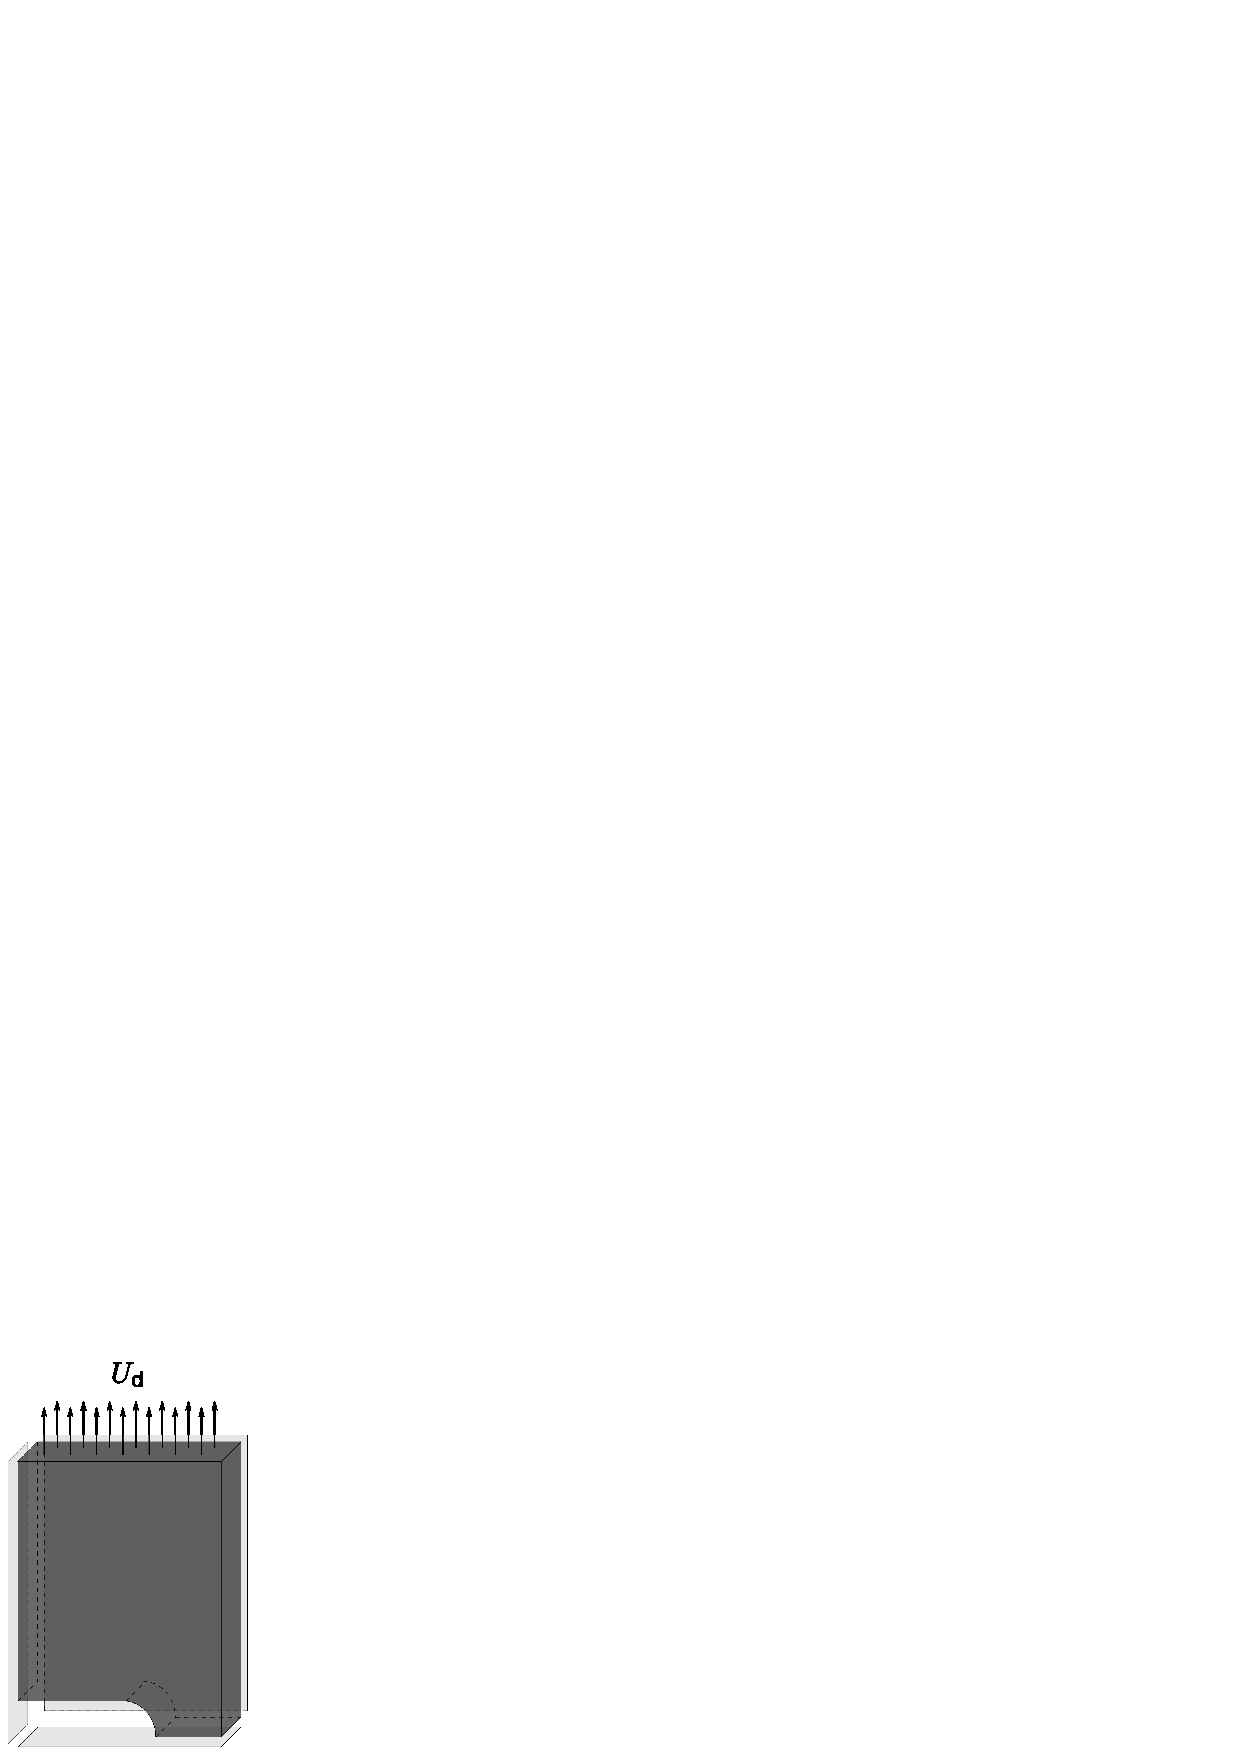
\includegraphics{./figures/3d_plate_1_8.pdf}
	\caption{A plate with a central groove subjected to cyclic loading.}
	\label{3dplate}
\end{figure}
Three examples are shown below. Firstly, a comparison with a standard incremental scheme for a cyclic load is presented where the error is computed for the quantity of interest (damage) rather than displacement. The proposed scheme is analysed in case of a periodic loading with variable amplitudes and frequencies. Lastly, a cyclic load with random amplitudes and large number of cycles is applied to the same model to test its capabilities.

\subsection{Model Verification}
\label{model_verification}

%ignore: \textbf{$ 1884 \cdot 41 \cdot 10 $ DOF}  \textbf{with respect to a modified Newton-Raphson to be fair because we are not updating the tangent ...}

The analysis of the plate, shown in \Cref{3dplate}, is carried out on a mesh that consists of $387$ hexahedron elements, with eight integration points in each element, resulting in $1884$ spatial displacement degrees of freedom. The model is subjected to a uniformly distributed displacement field with an amplitude of $U_0= 0.004\unit{mm}$. The time discretisation is chosen such that the temporal domain of each cycle is discretised into $200$ time steps. Since the whole temporal domain of each cycle is computed at once, a total of $376,800$ degrees of freedom are being sought. In the computational method, refer to \Cref{alg:latinpgd} for details, the convergence and the enrichment criteria are taken as $tol_1=10^{-14}$ and $tol_2=10^{-1}$, respectively. The simulation of the plate was carried out using a Newton-Raphson incremental scheme and the LATIN-PGD scheme. In order to initiate damage even from the first load cycle, the damage threshold is considered to be zero in this example, i.e., $\varepsilon_{p_{\rm D}} = 0$.

The prescribed load is illustrated in \Cref{fig_verification_load}. The corresponding damage evolution curve for the integration point with maximum damage as well as the corresponding error with respect to the incremental scheme are illustrated in \Cref{fig_verification_error}.
\begin{figure}[hbt!]
	\centering
	\begin{subfigure}[]{0.49\linewidth}
		\includestandalone{./figures/verify/prescribed_displacement}
		\caption{}
		\label{fig_verification_load}
	\end{subfigure}
	\hfil
	\begin{subfigure}[]{0.49\linewidth}
		\includestandalone{./figures/verify/damage_comparison}
		\caption{}
		\label{fig_verification_error}
	\end{subfigure}
	\caption{Verification with respect to an incremental scheme.  (\textbf{a}) the prescribed load; (\textbf{b}) damage evolution w.r.t. time along with the corresponding error.}
\end{figure}

The space-time average relative error, in \Cref{fig_ver_bochner}, is computed with the norm in Bochner space $L^2(\cT;L^2_\Omega)$ defined as
\begin{equation}
	\left\lVert {\fe} \right\rVert_{\Omega\times\cT}^2 = \frac{1}{T \ \abs{\Omega}} \intT \left\lVert \fe \right\rVert^2_{L^2_\Omega} \d t, \qquad \left\lVert \fe \right\rVert^2_{L^2_\Omega} = \intS \fe \dcontraction \fe \d \Omega.
\end{equation}
The fraction in front of the integral ensures preservation of the physical unit of $\fe$. The space-time averaging used to define a relative error, for different quantities of interest, over each load cycle are given in \Cref{fig_ver_bochner}.

A total of twelve PGD modes, see \Cref{fig_ver_pgdmodes}, were enough to maintain a relative error, in the maximum damage, below $0.15\%$. This error might be an outcome of using different temporal integration schemes between the incremental and semi-incremental algorithms. Note that the error in stress and strain quantities does not exceed $0.025\%$.
\begin{figure}[hbt!]
	\centering
	\begin{subfigure}[]{0.49\linewidth}
		\includestandalone{./figures/verify/error_space_time}
		\caption{}
		\label{fig_ver_bochner}
	\end{subfigure}
	\hfil
	\begin{subfigure}[]{0.49\linewidth}
		\includestandalone{./figures/verify/number_of_pgd_modes}
		\caption{}
		\label{fig_ver_pgdmodes}
	\end{subfigure}
	\caption{Verification with respect to an incremental scheme and the corresponding number of modes. (\textbf{a}) space-time average relative error w.r.t. number of cycles; (\textbf{b}) number of PGD modes w.r.t. the number of cycles.}
\end{figure}

The convergence behaviour of the proposed algorithm is illustrated in \Cref{fig_ver_vergence} where the number of iterations required to converge in each cycle and their corresponding error indicator values are depicted. The initial slow decrease in the error indicator, in the second cycle in \Cref{fig_ver_vergence}, is due to the update of the temporal functions before enriching the generated basis.
\begin{figure}[hbt!]
	\centering
	\begin{subfigure}[]{0.49\linewidth}
		\includestandalone{./figures/verify/error_indicator}
		\caption{}
		\label{fig_ver_vergence}
	\end{subfigure}
	\hfil
	\begin{subfigure}[]{0.49\linewidth}
		\includestandalone{./figures/verify/number_of_iterations}
		\caption{}
	\end{subfigure}
	\caption{Convergence and number of iterations. (\textbf{a}) error indicator w.r.t. number of iterations for each cycle; (\textbf{b}) number of iterations required to converge w.r.t. number of cycles.
	}
\end{figure}

To give an idea about the solution, which is sought in the online phase, the first temporal and spatial modes are depicted in \Cref{fig_ver_first_pair_mode}. The spatial mode, in this case, represents the equivalent strain which shows, as expected, localisation near the opening of the plate.
\begin{figure}[hbt!]
	\centering
	\begin{subfigure}[]{0.49\linewidth}
		\includestandalone{./figures/verify/first_temporal_mode}
		\caption{}
	\end{subfigure}
	\hfil
	\begin{subfigure}[]{0.49\linewidth}
		\hspace*{0.5cm}
		\includegraphics[width=.8\linewidth,height=28.5mm]{./figures/verify/first_strain_spatial_mode.png}
		\caption{}
	\end{subfigure}
	\caption{The first temporal and spatial modes. (\textbf{a}) the first temporal mode; (\textbf{b}) the first spatial equivalent strain mode.}
	\label{fig_ver_first_pair_mode}
\end{figure}

In these simulations, a speedup factor of 25, in favour of the semi-incremental scheme is obtained through the provided prototype implementation. The change in the memory footprint is negligible in the given example. However, it is worth noting that all the fields are stored over the whole temporal domain to simplify the comparison and postprocessing procedures. It is shown in the following examples that higher speedups are obtainable for a larger number of cycles.

%ignore: The damage distribution and the residual stress, at $t=120 \unit{sec}$, are plotted in \Cref{fig_distribution_12cycles}. As expected, the maximum damage is concentrated around the groove. In such a case, a combination of POD for the almost elastic structural response and PGD for the areas where nonlinearities are taking place could produce an effective scheme for damage computations.

\subsection{Variable Amplitude and Frequency Loading}
\label{var_ampl_freq}

%ignore: \textbf{Amplitudes: $[30,90]\cdot10^{-4}\unit{mm}$ \hfill Time periods: $[20,60]\unit{sec}$}

This example illustrates the capabilities of the proposed scheme and its numerical efficiency to simulate cyclic loads with variable amplitudes and frequencies. An increasing-decreasing load is investigated in this example where the higher the load amplitude is the shorter the time period, as seen in \Cref{fig_var_load}. The chosen load amplitudes belong to $[30,90]\cdot10^{-4}\unit{mm}$ while the time periods vary in $[20,60]\unit{sec}$. The time discretisation is chosen such that the temporal domain of each cycle is discretised into $40$ time steps. The convergence and the enrichment criteria are taken as $tol_1=10^{-3}$ and $tol_2=10^{-1}$, respectively. The damage threshold is considered to be zero, i.e., $\varepsilon_{p_{\rm D}} = 0$.

The damage evolution for the integration point with maximum damage is depicted in \Cref{fig_var_load_damage}. In order to better investigate the damage response in \Cref{fig_var_load_damage}, the damage increment in each load cycle is demonstrated in \Cref{fig_var_damageincrement}. It can be seen that \Cref{fig_var_damageincrement} is not symmetric due to the nonlinear response, which is driven by different initial conditions in each cycle and different values of the plastic strain rate. As expected, the maximum damage increment corresponds to the cycle with maximum load amplitude.
\begin{figure}[hbt!]
	\centering
	\begin{subfigure}[]{0.49\linewidth}
		\includestandalone{./figures/semi_incremental/temporal_scheme_2_1}
		\caption{}
		\label{fig_var_load}
	\end{subfigure}
	\hfil
	\begin{subfigure}[]{0.49\linewidth}
		\includestandalone{./figures/semi_incremental/temporal_scheme_2_2}
		\caption{}
		\label{fig_var_damage}
	\end{subfigure}
	\caption{Variable amplitude and frequency loading scenario.  (\textbf{a}) the prescribed load; (\textbf{b}) damage evolution w.r.t. the number of cycles.}
	\label{fig_var_load_damage}
\end{figure}

A maximum of eight PGD pairs are enough to obtain the aforementioned response, using an SVD orthonormalisation scheme presented in \Cref{optimised_pgd}. The number of PGD modes with respect to the number of cycles is shown in \Cref{fig_var_pgdmodes}.
\begin{figure}[hbt!]
	\centering
	\begin{subfigure}[]{0.49\linewidth}
		\includestandalone{./figures/semi_incremental/temporal_scheme_2_4}
		\caption{}
		\label{fig_var_pgdmodes}
	\end{subfigure}
	\hfil
	\begin{subfigure}[]{0.49\linewidth}
		\includestandalone{./figures/semi_incremental/temporal_scheme_2_3}
		\caption{}
		\label{fig_var_damageincrement}
	\end{subfigure}
	\caption{ROB size and damage increment with respect to the number of cycles.  (\textbf{a}) the growth of the PGD basis; (\textbf{b}) damage increment w.r.t. the number of cycles.}
	\label{fig_var_pgdmodes_damageincrements}
\end{figure}

%ignore: [carefull this is with accumulate, remove it and try again, the speedup should be higher] // The obtained speedup is this case is in the order of 10 compared to an estimated run of a classical incremental scheme.

It can be seen that the ROB size does not grow linearly with respect to the number of cycles and after simulating almost half of the cycles and facing all the different amplitudes and frequencies for the first time, the basis size does not further increase. However, if a Gram-Schmidt procedure is utilised, as in \Cref{fig_var_pgdmodes_gs}, the number of modes exceeds 55.
\begin{figure}[hbt!]
	\centering
	\includestandalone{./figures/semi_incremental/temporal_scheme_2_5}
	\caption{The growth of the ROB using a Gram-Schmidt scheme.}
	\label{fig_var_pgdmodes_gs}
\end{figure}


\subsection{Random Amplitudes Loading}
\label{eg_random_loading}
%ignore: \parencite{lemaitre2005engineering} 6.4.4 Stochastic Resolution by Monte Carlo Method // \textbf{$ 1884 \cdot 41 \cdot 10^4 $ DOF // $10^4$ cycles, uniform distribution in $[53,56]\cdot 10^{-2} \unit{mm}$ // $\text{Critical damage value } D_{\mathrm{c}}=0.3$\\ $\ \text{Probability of failure } P_{\mathrm{f}}=5.4\%$ // The mean and STD of $D_f$ // Requirements:\\ $[15-35]\unit{min}$ and $[1-1.5]\unit{GB}$ // Approx. 10 modes / Time-saving factors $50 \sim 100$}

This example shows a possible application of the proposed scheme where its efficiency can be put to the test. In this case, the plate (shown in \Cref{3dplate}) is subjected to a narrow-band variable loading with a time period $T=10\unit{sec}$. The uniformly distributed displacement for each cycle has a random value, i.e., the load is still cyclic, but the amplitudes are taken to follow a uniform distribution in the range $[0.0053,0.0056]\unit{mm}$.

In order to compute the probability of failure of the plate subjected to $10^4$ load cycles, the model is simulated under 2447 load realisations. The damage evolution for all realisations is depicted in \Cref{fig_random_damage}. The importance of the load sequence is easily seen in \Cref{fig_random_damage} where the change in the load amplitude and load sequence resulted in a final damage $D \in [0.20,0.41]$. The convergence of the mean and the standard deviation of the final damage value $D_{\mathrm{f}}^r$, at the end of the $10^4$ cycles, with respect to the number of Monte Carlo realisations ($r$) is illustrated in \Cref{fig_random_convergence}.
\begin{figure}[hbt!]
	\centering
	\begin{subfigure}[t]{0.49\linewidth}
		\includegraphics{./figures/semi_incremental/temporal_scheme_3_1.pdf}
		\caption{}
		\label{fig_random_damage}
	\end{subfigure}
	\hfil
	\begin{subfigure}[t]{0.49\linewidth}
		\includestandalone{./figures/semi_incremental/temporal_scheme_3_2}
		\caption{}
		\label{fig_random_convergence}
	\end{subfigure}
	\caption{Damage evolution driven by random amplitude loading. (\textbf{a}) damage w.r.t. number of cycles and 2447 load realisations; (\textbf{b}) the convergence of the mean and standard deviation of the final damage value.}
\end{figure}

The estimated standard error is computed as $\text{Std}(D_\mathrm{f}^r)/\sqrt{r} = 4.47 \times 10^{-4}$. Taking a confidence interval of three times the standard deviation around the mean, the final damage value is estimated as $D_{\mathrm{f}}^r=0.25 \pm 6\% \in [0.19,0.32]$. The probability of failure of the given structure is computed as the percentage of Monte Carlo trials in which the structure fails before reaching $10^4$ cycles. Assuming that the critical damage limit is taken as $\dc=0.3$, then the probability of failure is estimated as $5.4\%$.

In all the realisations, the number of modes did not exceed ten, and time-saving factors from 50 to 100, compared to an estimated run of a classical incremental scheme, are achieved. These simulations are run in parallel. However, one simulation takes $[15-35]\unit{min}$ and requires $[1-1.5]\unit{GB}$ random access memory (RAM) with the current implementation.
%ignore: 101000/(15*60) // 101000/(35*60) / debug on // 101000/(22*60) / debug off [speed up 76] // should give the value of alpha

\section{Summary}
To sum up, a semi-incremental extension to the LATIN-PGD method is proposed here. This extension shares similarities with the conventional incremental schemes and the non-incremental ones. Load cycles are simulated incrementally, which makes this scheme efficient to simulate fatigue damage problems. Additionally, a hybrid search direction is introduced to ensure the convergence of the algorithm. Examples with variable amplitude and frequency loadings were illustrated to show the capabilities of the proposed scheme.

\chapter{Optimality of Proper Generalised Decomposition Bases}
\label{optimised_pgd}

The greedy algorithms utilised to simulate structural problems with nonlinear material behaviour in a model order reduction framework are investigated in this chapter. In such a framework, adaptive strategies are interesting as they adjust the reduced order basis (ROB) to the problem of interest. However, these greedy strategies may lead to an excessive increase in the size of the ROB, i.e., the solution is no longer represented in its optimal low-dimensional expansion. Here, an optimised strategy is proposed to maintain, at each step of the greedy algorithm, the lowest dimension of a Proper Generalized Decomposition (PGD) basis using a randomised Singular Value Decomposition (SVD) algorithm. In comparison to conventional approaches such as Gram--Schmidt orthonormalisation or deterministic SVD, it is shown to be very efficient both in terms of numerical cost and optimality of the ROB. Examples with different mesh densities are investigated to demonstrate the numerical efficiency of the presented method. Note that the content of this chapter has been published in \parencite{Alameddin2019d}.

A posteriori model reduction techniques such as the Proper Orthogonal Decomposition (POD) is based on offline training computations which extract a reduced order basis (ROB) from the solution of a high fidelity model. This optimal basis is practically built through a singular value decomposition (SVD) of a snapshot matrix. The singular vectors corresponding to the highest singular values are used to build the ROB \parencite{cline2006computatio}. Then, the problem of interest is confined to this ROB, resulting in a drastic reduction in the numerical cost \parencite{chinesta2014separated,chinesta_encyclo_2018}. However, since the ROB has been defined as an optimal basis for the training stage, some advanced adaptive approaches are required to enrich the basis to tackle nonlinearities \parencite{kerfriden2011bridging}.

Proper Generalised Decomposition (PGD), which is a priori MOR technique, is based on the assumption that the quantities of interest can be written as a finite sum of products of separated functions, of generalised coordinates, which are sought in online computations \parencite{ladeveze1989large,chinesta2014separated}. No prior knowledge of the system is required in such a case, and the ROB is directly adapted to the problem of interest by using a greedy algorithm, which enriches the basis when required \parencite{Ladeveze2016227,bha2017}. However, an issue may be caused by the rapid growth of the ROB basis, whereas the primary interest of MOR is to benefit from a small-sized ROB which provides a nondemanding temporal updating step. This step is equivalent to a POD step where the spatial modes are fixed, and only the temporal modes are updated. It has been observed that the basis can increase to count some hundreds of modes for parametric studies of nonlinear cyclic loading \parencite{nasri2018proper}, or some thousands for parametric computations \parencite{ElHalabi2016a}. In \parencite{Heyberger2013b}, some advanced strategies have been proposed to use an optimal parametric path allowing for controlling the basis expansion.

In the context of reusing an ROB from a previous computation, a learning strategy has been proposed in {\parencite{ryckelynck2002reduction,ryckelynck2005priori}} to extract an optimal basis from the reduced order model (ROM) through a Karhunen--Lo\`{e}ve expansion. In a PGD framework, recompression based on SVD has been evaluated in \parencite{Giacoma2016}. However, the SVD step turns out to be numerically expensive, prohibiting its implementation at each iteration. Therefore, it is common to let the basis increase and compress the results only at convergence to decrease their storage requirements. Therefore, it appears of interest to investigate probabilistic algorithms to compress the ROB on-the-fly without creating a bottleneck in the ROM. A detailed review of the most established algorithms to compute an SVD is provided in \parencite{Golub_VanLoan_1996,Bach_Ceglia_2018}. These algorithms are not limited to conventional deterministic methods such as truncated, incremental or iterative SVD but also include randomised algorithms \parencite{halko2011finding}. Different algorithms have been tested for POD applications in the case of dynamical problems in \parencite{Bach_Ceglia_2018}. It has been noticed that randomised SVD algorithms can drastically reduce the numerical cost of the decomposition required after the training stage. Even if this step occurs only once in the offline stage of POD based ROM, the number of degrees of freedom and time steps can be vast for the high fidelity model so that the decomposition process can be a bottleneck.

Our goal here is to maintain the flexibility of the greedy algorithm through the usage of PGD while controlling the size of the ROB with a minimal numerical cost, by proposing to use a randomised SVD algorithm that provides a nondemanding compressive step after each enrichment of the basis. The numerical approach will be herein exemplified for the specific case of a fatigue computation based on continuum damage mechanics in a large time increment (LATIN) framework. However, the proposed numerical strategy can be generally used to optimise PGD basis for any application efficiently.

This chapter is structured as follows. Discussion on the optimality of the PGD modes and the different algorithms to ensure that is provided in \Cref{sec_orth} followed by different numerical examples, in \Cref{sec_examples}, to illustrate the robustness and efficiency of the proposed algorithm.

\section{Optimality of the Generated ROB}
\label{sec_orth}
Recall that the correction/solution at the i\textsuperscript{th} iteration of the LATIN algorithm, in matrix notation, reads

\begin{equation}
	\z{\mat{U}} = \ds \sum_{j=1}^{\mu} \vv_j \ \T{\vlambda}_j = \mV \ \T{\mLambda} \in \ffR^{n\times n_t},
	\label{eq_outer_prod}
\end{equation}
where $\mV=[\vv_1,\cdots,\vv_{\mu}] \in \ffR^{n\times \mu} $ and $\mLambda=[\vlambda_1,\cdots,\vlambda_{\mu}] \in \ffR^{n_t \times \mu} $. The representation in \Cref{eq_outer_prod} is referred to as an outer-product form \parencite{Bebendorf2008}, and such a form only requires the storage of $\mu(n+n_t)$ entries to represent $\z\mU$ with $n n_t$ entries. It is practical to orthonormalise the spatial functions $\vv_j$ before generating the temporal ones in order to limit the ROB size, i.e., the PGD expansion. This is traditionally done via a Gram--Schmidt (GS) procedure \parencite{bha2017}. An orthonormalisation scheme based on a GS procedure is summarised in \Cref{alg:gramschmidt}, where $\T{\vv}_l \ {\vv}_m = \delta_{lm}$ is the inner product between the spatial modes, $\delta_{lm}$ is the Kronecker delta and ${\lVert{\vv_j}\rVert}_2^2=\T{\vv}_j \ {\vv}_j$.

\begin{algorithm}[hbt!]
	\KwData {\begin{tabular}{ll}
			\normalsize \ Previously generated modes & \normalsize $\{\vv_j, \vlambda_j\} \, (j=1,\cdots,\mu)$ with $\T{\vv}_l \ {\vv}_m = \delta_{lm}$ \\
			\normalsize \ New pair of modes          & \normalsize $\{\vv_{\mu+1}, \vlambda_{\mu+1}\}$
		\end{tabular}}
	\vspace{0.2cm}
	\KwResult{Enriched basis $\{\vv_j, \vlambda_j\} \, (j=1,\cdots,\mu+1)$ with $\T{\vv}_l \ {\vv}_m = \delta_{lm}$}
	\vspace{0.2cm}
	\For{$j\leftarrow 1$ \KwTo $\mu$}{
	Calculate the inner product of ${\vv}_{\mu+1}$ and an existing mode via $p=\T{\vv}_j \ {\vv}_{\mu+1}$\\
	Subtract the projection from the new mode via $\vv_{\mu+1} \leftarrow \vv_{\mu+1} - p \ \vv_j$\\
	Update existing temporal mode $\vlambda_{j}=\vlambda_j+p \ \vlambda_{j+1}$
	}
	Normalise the new spatial mode $v_{\mu+1} \leftarrow v_{\mu+1}/{\lVert{\vv_{\mu+1}}\rVert}_2$\\
	Update the new temporal mode $\lambda_{\mu+1} \leftarrow \lambda_{\mu+1} \ {\lVert{\vv_{\mu+1}}\rVert}_2$
	\caption{Gram--Schmidt based orthonormalisation procedure}
	\label{alg:gramschmidt}
\end{algorithm}

While experimenting on the LATIN-PGD scheme in a three-dimensional finite element framework, it has been noticed that reaching a low error required generating many modes. Further discussion about the computational cost is provided in \Cref{sec_examples}. This confirms the findings in \parencite{Giacoma2015} that orthonormality of the spatial modes is not enough to confine the PGD expansion, i.e., compressing the spatial modes only, leaves the temporal modes susceptible to redundancy.

\subsection{SVD Compression of PGD}

As long as PGD is not a unique decomposition and does not ensure the optimality of the generated modes in terms of a minimal expansion, an optimal decomposition can be obtained via an SVD of the full solution \parencite{Eckart1936}.  An SVD of the solution provides a straightforward scheme to compress both spatial and temporal information into a minimal set of modes, following \Cref{alg:svd}. This is similar to compressing information from different spatial directions into a single spatial mode.

It is known via the Schmidt--Eckart--Young theorem that the solution $\z{\mU}$ has an optimal approximation of rank $k\leq\mu+1$ with respect to the Frobenius norm that satisfies \parencite{Bebendorf2008}

\begin{equation}
	{\lVert \z{\mU} - \z{\mU}^{(k)} \rVert}_\mathrm{F} = \ds \sum_{j=k+1}^{\mu+1} \z{s}_j^2.
	\label{eq_approx_error}
\end{equation}
The corresponding approximation error in terms of the spectral norm reads

\begin{equation}
	{\lVert \z{\mU} - \z{\mU}^{(k)} \rVert}_\mathrm{2} = \z{s}_{k+1}.
	\label{eq_approx_error_spectral}
\end{equation}
Hence, the PGD expansion may be restricted to a maximum number of modes and \Cref{eq_approx_error,eq_approx_error_spectral} will give a measure of the approximation error due to this enforced truncation. Another way is to prescribe a subjectively acceptable tolerance $\epsilon_{\mathrm{tol}}$ that the approximation error should not exceed, e.g., in the spectral norm this renders to

\begin{equation}
	\frac{{\lVert \z{\mU} - \z{\mU}^{(k)} \rVert}_\mathrm{2}}{{\lVert \z{\mU} \rVert}_\mathrm{2}} = \frac{\z{s}_{k+1}}{\z{s}_1} < \epsilon_{\mathrm{tol}}.
\end{equation}

\begin{algorithm}[hbt!]
	\KwData {\begin{tabular}{ll}
			\normalsize \ Previously generated modes             & \normalsize $\{\vv_j, \vlambda_j\} \, (j=1,\cdots,\mu)$ \\
			\normalsize \ New pair of modes                      & \normalsize $\{\vv_{\mu+1}, \vlambda_{\mu+1}\}$         \\
			\normalsize \ Number of modes / truncation threshold & \normalsize ${k\leq\mu+1}, \ \epsilon_{\mathrm{tol}}$   \\
		\end{tabular}}
	\vspace{0.2cm}
	\KwResult{Enriched basis $\{\vv_j, \vlambda_j\} \, (j=1,\cdots,k)$ with $\T{\vv}_l \ {\vv}_m = \delta_{lm}$}
	\vspace{0.2cm}

	Compute the full solution $\tilde{\mU} = \mV \ \T{\mLambda}$\\
	Compute a thin/truncated SVD of the solution $\tilde{\mU}^{(\mu+1)} = \ds\sum_{j=1}^{\mu+1} \z{s}_j \ \z\vv_j \ \T{\z\vlambda}_j$\\
	Truncate the decomposition based on $\z{s}_{k+1}/\z{s}_1< \epsilon_{\mathrm{tol}}$ or directly using $k$\\
	Recover the outer-product representation:\\
	\qquad $\mV \leftarrow [\z\vv_1,\cdots,\z\vv_{k}] \in \ffR^{n\times k} $\\[0.1cm]
	\qquad $\mLambda \leftarrow [\z{s}_1\ \z\vlambda_1,\cdots,\z{s}_k\ \z\vlambda_{k}] \in \ffR^{n_t \times k} $

	\caption{SVD compression of a PGD expansion}
	\label{alg:svd}
\end{algorithm}

The computation of a full SVD, in case of $n>n_t$, requires ${\cal O}(nn_t^2)$ floating point operations (flops) while seeking a truncated SVD requires ${\cal O}(nn_t k)$ flops. Due to the high computational cost of applying an SVD at each enrichment step in a PGD context, a quasi-optimal iterative orthonormalisation scheme was proposed in \parencite{Giacoma2015,Giacoma2016}. However, another appealing, straightforward approach to provide a direct compression of the PGD modes into a minimal set is utilised here. It consists of using a randomised SVD algorithm \parencite{halko2011finding} to compress the PGD expansion.

\subsection{Randomised SVD (RSVD) Compression of PGD}

Low-rank matrix decompositions may be computed efficiently using randomised algorithms as illustrated in this section for an SVD case. Such methods are based on random sampling to approximate the range of the input matrix, i.e., a subspace that captures most of the matrix effect. Then, the matrix is restricted to this subspace, and the low-rank approximation of this reduced matrix is sought using classical deterministic schemes. If $\z{\mU}$ is a dense matrix, the required flops are reduced from ${\cal O}(nn_tk)$ to ${\cal O}(nn_t\log{(k)})$, where $k$ is the number of the sought dominant singular values of an $n\times n_t$ matrix. It is worth mentioning that, even when randomised algorithms require a higher number of flops, they exploit modern multi-processor architecture more efficiently than standard deterministic schemes \parencite{halko2011finding}. {It has been shown in \parencite{Bach_Ceglia_2018} that a randomised SVD algorithm can outperform a truncated SVD one with a speedup factor over 50 when $k=10$.} An overview of the randomised SVD algorithm applied in a PGD context is briefed in \Cref{alg:randomised_svd}.

\begin{algorithm}[hbt!]
	\KwData {\begin{tabular}{ll}
			\normalsize \ Previously generated modes & \normalsize $\{\vv_j, \vlambda_j\} \, (j=1,\cdots,\mu)$ \\
			\normalsize \ New pair of modes          & \normalsize $\{\vv_{\mu+1}, \vlambda_{\mu+1}\}$
		\end{tabular}}
	\vspace{0.2cm}
	\KwResult{Enriched basis $\{\vv_j, \vlambda_j\} \, (j=1,\cdots,k)$ with $\T{\vv}_l \ {\vv}_m = \delta_{lm}$}
	\vspace{0.2cm}

	Compute the full solution $\z{\mU} = \mV \ \T{\mLambda} \in \ffR^{n\times n_t}$\\
	Approximate a basis $\mE$ of $\mathrm{range}(\z{\mU})$ via $\mE \leftarrow \z{\mU} \ \mQ \in \ffR^{n\times\z{k}}$ with\\
	\qquad $\mQ \in \ffR^{n_t\times\z{k}}$ is a random matrix, $\z{k}=k+p$ and $p$ is an oversampling factor taken\\ \qquad experimentally to be in the range of $5\sim10$ \parencite{halko2011finding}.\\
	Orthonormalise the columns of $\mE$ such that $\z{\mU} \approx \mE \ \T{\mE} \z{\mU}$.\\
	Restrict $\z{\mU}$ to the $\mathrm{span\{col(} \mE)\}$ to get a small matrix ${\mS=\T{\mE} \z{\mU} } \in \ffR^{\z{k}\times n_t}$\\
	Compute a truncated SVD ${\mS \approx \mS^{(k)} = {\z{\z{\mV}}} \ \z\mS \ \T{\z\mLambda}}$ with ${k\leq\mu+1}$\\
	Expand $\mS$ to $\mathrm{span\{col(} \z{\mU})\}$, i.e., ${\z{\mU} \approx \mE \ {\mS^{(k)} = }  \mE \ {\z{\z{\mV}}} \ \z\mS \ \T{\z\mLambda} = \z{\mV} \ \z\mS \ \T{\z\mLambda}}$\\
	Recover the outer-product representation:\\
	\qquad $\mV \leftarrow [\z\vv_1,\cdots,\z\vv_{k}] \in \ffR^{n\times k} $\\[0.1cm]
	\qquad $\mLambda \leftarrow [\z{s}_1\ \z\vlambda_1,\cdots,\z{s}_k\ \z\vlambda_{k}] \in \ffR^{n_t \times k} $

	\caption{RSVD compression of a PGD expansion}
	\label{alg:randomised_svd}
\end{algorithm}

\Cref{alg:randomised_svd} can be straightforwardly extended to sample the rows of $\z{\mU}$ when $n_t$ is large. However, this is not the case in the current study. It is also possible to exploit the PGD decomposition of the solution when computing its SVD or RSVD \parencite{Bebendorf2008}; see \Cref{alg:svd_decomposition} for details.

\begin{algorithm}[hbt!]
	\KwData {\begin{tabular}{ll}
			\normalsize \ Previously generated modes             & \normalsize $\{\vv_j, \vlambda_j\} \, (j=1,\cdots,\mu)$ \\
			\normalsize \ New pair of modes                      & \normalsize $\{\vv_{\mu+1}, \vlambda_{\mu+1}\}$         \\
			\normalsize \ Number of modes / truncation threshold & \normalsize ${k\leq\mu+1}, \ \epsilon_{\mathrm{tol}}$   \\
		\end{tabular}}
	\vspace{0.2cm}
	\KwResult{Enriched basis $\{\vv_j, \vlambda_j\} \, (j=1,\cdots,k)$ with $\T{\vv}_l \ {\vv}_m = \delta_{lm}$}
	\vspace{0.2cm}

	QR-decomposition:\\
	\qquad $\mV =  \mQ_v \ \mR_v \qquad \sim{\cal O} ((\mu+1)^2 \ n)$\\
	\qquad $\mLambda = \mQ_\lambda \ \mR_\lambda \qquad \sim {\cal O} ((\mu+1)^2 \ n_t)$    \\
	Compute $\mR_v \ \T{\mR}_\lambda \in \ffR^{(\mu+1)\times(\mu+1)}$\\
	Apply \Cref{alg:randomised_svd} to approximate $\mR_v \ \T{\mR}_\lambda$ as $\ds\sum_{j=1}^{k} \z{s}_j \ \z\vv_j \ \T{\z\vlambda}_j$  \\
	Recover the outer-product representation:\\
	\qquad $\mV \leftarrow \mQ_v \ \z{\mV} \in \ffR^{n\times k} $\\[0.1cm]
	\qquad $\mLambda \leftarrow  \mQ_\lambda \ \z\mLambda \ \T{\z{\mS}} \in \ffR^{n_t \times k} $

	\caption{RSVD compression that exploits the PGD expansion (RSVD-PGD)}
	\label{alg:svd_decomposition}
\end{algorithm}

\Cref{alg:svd_decomposition} utilises a rank revealing QR-decomposition in order to not rebuild the full matrix $\z{\mU}$. Further algorithmic details of the presented deterministic and randomised algorithms may be found in \parencite{Golub_VanLoan_1996,Bach_Ceglia_2018,halko2011finding}. However, the goal of this study is to investigate the behaviour, robustness and efficiency of the presented algorithms in a PGD framework.

\section{Numerical Results}
\label{sec_examples}

The different algorithms are tested on the example introduced in \Cref{model_verification}. Three examples are discussed below. Firstly, the effect of the temporal function update is investigated; see \Cref{sec_time_update}. Then, the PGD behaviour with different orthonormalisation schemes is analysed to illustrate the optimality of the ROB. Lastly, the computational requirements of the orthonormalisation schemes and their effect on the temporal function update are discussed.

\subsection{Temporal Function Update}
The analysis of the plate, shown in \Cref{3dplate}, is carried out on a mesh that consists of $387$ hexahedron elements, with eight integration points in each element, resulting in $1884$ spatial displacement degrees of freedom. The model is subjected to a uniformly distributed displacement field with an amplitude $U_0= 0.00606 \unit{mm}$ and a time period $T = 10 \unit{sec}$. The temporal discretisation is chosen such that the domain $[0,T]$ is discretised into $33$ time steps. Since the whole time domain is computed at once, a total of $62,172$ degrees of freedom are being sought. The commonly used GS scheme (\Cref{alg:gramschmidt}) is utilised in this example, and the convergence criterion is considered to be $10^{-10}$.

The purpose of this test case is to evaluate the importance of the updating step in a PGD approach. Hence, the number of generated modes along with the number of the LATIN iterations, with and without this temporal update step, are illustrated in \Cref{fig_time_update}.

\begin{figure}[hbt!]
	\centering
	\begin{subfigure}[]{0.49\linewidth}
		\includestandalone{./figures/modal_optimisation/mgs_1cycle_no_update_pgd_number}
		\caption{}
	\end{subfigure}
	\hfil
	\begin{subfigure}[]{0.49\linewidth}
		\includestandalone{./figures/modal_optimisation/mgs_1cycle_update_pgd_number}
		\caption{}
	\end{subfigure}
	\caption{The size of the generated ROB. (\textbf{a}) {ROB}
		size without the updating step; (\textbf{b}) ROB size with the updating step.}
	\label{fig_time_update}
\end{figure}

It is seen in \Cref{fig_time_update} {that the required number of LATIN iterations} is not affected by this updating step, but the computational cost is sharply decreased. Moreover, such a step is crucial to limit the size of the PGD expansion. With the updating step, only half the number of modes were generated in comparison with the approach without any update. Due to this favourable nature, the updating step is implemented in the rest of the examples.

\subsection{PGD Behaviour with Different Orthonormalisation Schemes}
The previous example with the same spatial discretisation is subjected to $12$ load cycles with different amplitudes, in the range of $[0.0033,0.0066]\unit{mm}$. The temporal domain is divided into $12$ intervals, each corresponding to one cycle, and the ROB generated within one cycle is reused in the following cycles. The convergence criterion is considered to be $10^{-4}$.

The nonlinearity and the rapid damage evolution can be seen in \Cref{fig_damage_evolution12cycles_chapter6} where the damage value at the end of each cycle is plotted with respect to the number of cycles. The first PGD temporal function of each cycle, after convergence, is illustrated in \Cref{fig_pgdtemporal12cycles}.

\begin{figure}[hbt!]
	\centering
	\begin{subfigure}[]{0.49\linewidth}
		\includestandalone{./figures/modal_optimisation/12_cycles_mgs_damage_evolution}
		\caption{}
		\label{fig_damage_evolution12cycles_chapter6}
	\end{subfigure}
	\hfil
	\begin{subfigure}[]{0.49\linewidth}
		\includestandalone{./figures/modal_optimisation/12_cycles_mgs_time_modes}
		\caption{}
		\label{fig_pgdtemporal12cycles}
	\end{subfigure}
	\caption{Damage evolution and the first {PGD}
		temporal mode in each cycle. (\textbf{a}) damage w.r.t. number of cycles; (\textbf{b}) first temporal function.}
\end{figure}

The simulation is carried out using \Cref{alg:gramschmidt,alg:svd,alg:svd_decomposition,alg:randomised_svd} and the resulting number of PGD modes with respect to the number of cycles is depicted in \Cref{fig_number_pgd_modes_12cycles}. It is shown in \Cref{fig_number_pgd_modes_12cycles_mgs} that using \Cref{alg:gramschmidt} resulted in an ROB with $18$ modes while  \Cref{alg:svd,alg:svd_decomposition,alg:randomised_svd} reduced this number to $11$ modes by adding a maximum of one supplementary mode for each cycle. It is emphasised that \Cref{alg:svd,alg:svd_decomposition,alg:randomised_svd} provide the same ROB. However, their computational cost differs as illustrated in \Cref{sec_svd_results}.

\begin{figure}[hbt!]
	\centering
	\begin{subfigure}[]{0.49\linewidth}
		\includestandalone{./figures/modal_optimisation/12_cycles_mgs_number_of_pgd_modes}
		\caption{}
		\label{fig_number_pgd_modes_12cycles_mgs}
	\end{subfigure}
	\hfil
	\begin{subfigure}[]{0.49\linewidth}
		\includestandalone{./figures/modal_optimisation/12_cycles_svd_number_of_pgd_modes}
		\caption{}
	\end{subfigure}
	\caption{Number of PGD modes in each cycle using different orthonormalisation schemes. (\textbf{a}) number of PGD modes using {GS}; (\textbf{b}) number of PGD modes using {(R)SVD}.}
	\label{fig_number_pgd_modes_12cycles}
\end{figure}

It is observed that an SVD compression provides optimality of the ROB. It also has interesting properties, such as not rejecting any mode in the current example. In other words, due to the optimality of the generated ROB, the temporal update step plays a prominent role in convergence, and there is no need for further enrichment of the ROB.

The inner product of the spatial modes in each case, after the last cycle, with their corresponding SVD of the acquired solution is shown in \Cref{fig_modes_optimality}. As expected, the GS modes are far from the optimal SVD ones while, trivially, \Cref{fig_svd_optimality} depicts an almost diagonal matrix. The off-diagonal entries are caused by the update of the temporal functions at the final iterations.

\begin{figure}[hbt!]
	\centering
	\begin{subfigure}[t]{0.31\linewidth}
		\includegraphics{./figures/modal_optimisation/gs_optimality}
		\caption{}
	\end{subfigure}
	\hfil
	\begin{subfigure}[t]{0.31\linewidth}
		\includegraphics{./figures/modal_optimisation/svd_optimality}
		\caption{}
		\label{fig_svd_optimality}
	\end{subfigure}
	\hfil
	\begin{subfigure}[t]{0.31\linewidth}
		\includegraphics{./figures/modal_optimisation/svd_update_optimality}
		\caption{}
		\label{fig_svd_update_optimality}
	\end{subfigure}
	\caption{ROB optimality w.r.t. an SVD of the resulting solution. (\textbf{a}) GS; (\textbf{b}) (R)SVD; (\textbf{c}) e(R)SVD.}
	\label{fig_modes_optimality}
\end{figure}

It is of interest to point out that the usage of an (R)SVD scheme at every LATIN iteration after the temporal function update or the enrichment of the basis restricts the ROB to six modes only as illustrated {in} \Cref{fig_svd_update_optimality}. The introduced usage of (R)SVD at every iteration is referred to afterwards as excessive (R)SVD and abbreviated as e(R)SVD.

\subsection{Relative Performance of the Different Orthonormalisation Schemes}
\label{sec_svd_results}

The ensured optimality of the ROB is of interest when used with challenging examples such as in many-query context, due to the expected slow growth of the ROB. In order to investigate the robustness and the behaviour of the ROB, in a many-query context with a large number of degrees of freedom, the plate model is discretised into 13,812 hexahedron elements, with eight integration points in each element, resulting in $50,547$ spatial displacement degrees of freedom. The temporal discretisation consists of $33$ time step{s} in each cycle resulting in $1,668,051$ degrees of freedom in each cycle. The plate is subjected to a uniformly distributed displacement field with a uniformly distributed random amplitudes in the range of $[18,22]\times 10^{-5} \unit{mm}$ and a time period $T = 10 \unit{sec}$. The convergence criterion is considered to be $10^{-4}$.

The resulting number of PGD modes with respect to the number of cycles using GS and SVD algorithms is illustrated in \Cref{fig_100cycles_number_of_modes_1,fig_100cycles_number_of_modes_2}. It is seen that using a GS algorithm allows the ROB to grow to contain $126$ pairs of modes while SVD algorithms confine this size to $21$ modes, using a truncation threshold of $10^{-8}$. Accepting a bigger approximation error with a truncation threshold of $10^{-5}$ reduces the number of modes to $11$ pairs while an e(R)SVD scheme introduces further reduction to seven modes without any rejection or truncation due to the maintained optimality of the ROB.

\begin{figure}[hbt!]
	\centering
	\begin{subfigure}[t]{0.49\linewidth}
		\includestandalone{./figures/modal_optimisation/mgs_number_of_pgd_modes}
		\caption{}
	\end{subfigure}
	\hfil
	\begin{subfigure}[t]{0.49\linewidth}
		\includestandalone{./figures/modal_optimisation/svd_m8_number_of_pgd_modes}
		\caption{}
	\end{subfigure}
	\caption{ROB size using different orthonormalisation algorithms. (\textbf{a}) number of PGD modes using GS; (\textbf{b}) number of PGD modes using (R)SVD ($\epsilon_{\mathrm{tol}}=10^{-8}$).}
	\label{fig_100cycles_number_of_modes_1}
\end{figure}


\begin{figure}[hbt!]
	\centering
	\begin{subfigure}[t]{0.49\linewidth}
		\includestandalone{./figures/modal_optimisation/svd_m5_number_of_pgd_modes}
		\caption{}
	\end{subfigure}
	\hfil
	\begin{subfigure}[t]{0.49\linewidth}
		\includestandalone{./figures/modal_optimisation/excessive_svd_m8_number_of_pgd_modes}
		\caption{}
	\end{subfigure}
	\caption{ROB size using different orthonormalisation algorithms. (\textbf{a}) number of PGD modes using (R)SVD ($\epsilon_{\mathrm{tol}}=10^{-5}$); (\textbf{b}) number of PGD modes using e(R)SVD.}
	\label{fig_100cycles_number_of_modes_2}
\end{figure}

It is worth noting that, in this example, the SVD orthonormalisation schemes, other than e(R)SVD, were invoked only $53$ times compared to $125$ times with the GS algorithm. Hence, this explains the low computational requirements of \Cref{alg:svd,alg:svd_decomposition,alg:randomised_svd} in comparison with \Cref{alg:gramschmidt} as summarised in \Cref{fig_orthonormalisation_cost}. The e(R)SVD scheme was invoked in each LATIN iteration. However, due to the small number of generated modes, the required time to update the temporal functions is drastically low in comparison with the other schemes; see \Cref{fig_update_cost}.

\begin{figure}[hbt!]
	\centering
	\begin{subfigure}[t]{0.49\linewidth}
		\includestandalone{./figures/modal_optimisation/temporal_update_timing}
		\caption{}
		\label{fig_update_cost}
	\end{subfigure}
	\hfil
	\begin{subfigure}[t]{0.49\linewidth}
		\includestandalone{./figures/modal_optimisation/orthonormalisation_timing}
		\caption{}
		\label{fig_orthonormalisation_cost}
	\end{subfigure}
	\caption{The required time to perform the temporal update and the orthonormalisation steps. (\textbf{a}) timing of the temporal function update; (\textbf{b}) timing of orthonormalisation schemes.}
	\label{fig_numerical_cost_update}
\end{figure}

It is worth noting that the timing for each algorithm depends on the available computational resources. However, we expect their relative performance to remain unchanged. The RSVD algorithm is implemented in MATLAB\textsuperscript{\textregistered} and uses its built-in SVD routine.

\subsubsection{Comparison between Deterministic and Randomised SVD Schemes}

It is clear from \Cref{fig_numerical_cost_update} that all deterministic and randomised SVD schemes are of interest to compress the PGD expansion on-the-fly. Below is an example that illustrates the difference between \Cref{alg:svd,alg:randomised_svd} in case of two synthetic matrices $\mat{M}_1 \in \ffR^{10^{6}\times10^{2}}$ and $\mat{M}_2 \in \ffR^{10^{6}\times10^{3}}$. Note that this example reproduces results from the literature to give an idea of possible speedups using a MATLAB\textsuperscript{\textregistered} implementation. The cost to extract the first 10, 20 and 30 singular vectors is recorded and summarised in \Cref{fig_synthetic_matrix_svd}.

\begin{figure}[hbt!]
	\centering
	\begin{subfigure}[t]{0.49\linewidth}
		\includestandalone{./figures/modal_optimisation/svd_small_matrix}
		\caption{}
	\end{subfigure}
	\hfil
	\begin{subfigure}[t]{0.49\linewidth}
		\includestandalone{./figures/modal_optimisation/svd_big_matrix}
		\caption{}
	\end{subfigure}
	\caption{The required time to extract the first 10,20 and 30 singular vectors using SVD and RSVD. (\textbf{a}) timing of modal extraction from $M_1$; (\textbf{b}) timing of modal extraction from $M_2$.}
	\label{fig_synthetic_matrix_svd}
\end{figure}

\section{Summary}
\label{sec_conclusion}

Different orthonormalisation techniques were investigated to ensure the optimality of the PGD decomposition. These techniques and their effect on the PGD greedy algorithm are illustrated throughout examples with a varying number of degrees of freedom. It is found that a randomised SVD algorithm is a promising scheme to ensure the optimality of PGD expansions. Beneficial time reduction is introduced by limiting the number of modes compared to a Gram--Schmidt procedure. Another promising approach is proposed here where the randomised SVD scheme is invoked at each LATIN iteration, after the temporal update or the basis enrichment. This approach is referred to, in the current work, as e(R)SVD and it shows desired properties such as ensuring an optimal basis in each iteration and {reducing the enrichment of basis functions to a minimum}, i.e., no modes are rejected. The proposed numerical strategy, though it is presented in a LATIN-PGD framework, can be used to optimise PGD basis for any application.


\chapter{Data Assisted Modelling}
\label{data_assisted}

A detailed investigation of the numerical costs of the solution algorithm developed in this work is carried out in this chapter. The goal is to define any leftover computational bottlenecks and suggest different approaches to alleviate such challenges. It is worth noting that the first part of this section is devoted to algorithmic discussion built on observations of the developed implementation while the second part goes further to investigate the pros and cons of utilising some machine learning techniques.

The problem, introduced in \Cref{model_verification} is used here as a reference problem with a change in the convergence criterion to be $10^{-4}$. Also, finer spatial and temporal discretisations are introduced for a final evaluation.

\section{Discussion on the Numerical Cost and Further Reduction}
\label{sec7_further_reduction}

The timings of the problem introduced in \Cref{model_verification} are summarised in \Cref{tab_timing}. The numbers show that the first goal to reduce the cost of solving the global stage has already been achieved because this stage spans only $8 \percent$ of the computational time. The dominant parts are now localised in the evaluation of the constitutive model in the local stage, requiring $33 \percent$ of the total time, and the evaluation of the error indicator at each iteration, consuming another $33 \percent$ of the total time.

\begin{table}[hbt!]
	\caption{Relative timing of the main algorithmic stages.}
	\label{tab_timing}
	\centering
	\begin{tabular}{ll}
		\toprule
		\textbf{Algorithmic step}                        & \textbf{Relative timing} \\
		\midrule
		Evaluation of the local stage                    & $33 \percent$            \\
		Evaluation of the global stage                   & $8 \percent$             \\
		Evaluation of the error indicator                & $33 \percent$            \\
		The rest (initialisation, input and output, ...) & $26 \percent$            \\
		\bottomrule
	\end{tabular}
\end{table}

A first glance at \Cref{tab_timing} reveals that the demanding evaluation of the error indicator in every iteration is a result of integrations over spatial and temporal domains over and over again, while the cost of the local stage is driven by evaluation of a sophisticated nonlinear material model.

\section{Evaluation of the Error Indicator}
A straight forward approach to reduce the numerical cost of evaluating the error indicator in cases of variable loading scenarios, where convergence is not expected to occur from the first iteration, is to evaluate the error indicator only at specific iterations. Hence, a new parameter is introduced in the numerical scheme that controls when the error indicator is evaluated, either being every two iterations or every five iterations, for instance. As an outcome, the evaluation of the error indicator, in the example above, is reduced from $33 \percent$ to only $15 \percent$. In other words, the demanding evaluation of the error indicator is traded for more non-demanding linear iterations.

Further reduction of the requirements of the numerical scheme may be achieved by exploiting the outer-product form in the numerical integration. Such exploitation is based on the assumption that all quantities of interest, local and global stresses and strains are written in an outer-product format, as introduced below.

\section{Decomposition of Quantities of Interest}

Even though the strain in \Cref{eq_sa01} is written in an outer-product format using PGD, the derived stress through \Cref{eqstresscorrection} is not decomposed due to the involvement of the dense residual $\fhf_k$ from the local stage. Hence, the stress is stored entirely for the whole spatial and temporal domains along with the stress and strain increments, used in the computation of the error indicator. In addition, the error indicator formulation, \Cref{eq_error_indicator}, requires the storage of four tensorial variables for each time-space point which renders the computational cost of evaluating this indicator as expensive and might even exceed the cost of performing the global stage computations, as illustrated in \Cref{tab_timing}. Hence, it is proposed here to keep the stress and strain in an outer-product format to lower the storage requirements and ease the computational use of these variables.

Writing the stress in an outer-product format requires decomposing the obtained stress into spatial and temporal functions. Hence, the residual in \Cref{eqstresscorrection} has to be decomposed as well. Starting from a decomposed elastic solution, the residual, defined in \Cref{eq:stress_correction}, can be decomposed by decomposing the stress and strain coming from the local stage.

Intrusive non-supervised decomposition of the stress and strain in every local stage leads to error stagnation due to the transition from the full state to the low-rank approximation and vice versa, besides its demanding cost. In other words, the scheme is susceptible to lose information, at each iteration, due to the compression of the quantities of interest. However, in the case of horizontal search direction, what is needed is to decompose the local strain once at every iteration then the stress correction in \Cref{eq:stress_correction} is automatically decomposed and the loss of information is confined to one step only.

The proposed decomposition is expected to lower the algorithmic evaluation of arithmetic operations on low-rank matrices, reduce the memory consumption and the cost of evaluating the error indicator.

\subsection{Modifications Applied to the Local Stage}
The goal here is to introduce the stress and strain decompositions into the local stage such that the resulting residual is written in an outer-product format and consequently the stress in the global stage. In the local stage, stress and damage come into interaction in \Cref{eq_state_eq,eq_yield_func}, for instance. In cases where the stress is decomposed, but the damage is not, the quantity $(1/(1-D))$ is decomposed and written in a low-rank matrix that triggers only multiplicative operations in PGD format. An alternative approach would be to approximate the damage as a rank-one matrix which allows it to be used with division operators and still does not enforce any constraints on the outcome of the local stage with damage values satisfying the constitutive model.

The strain in the local stage still has to be decomposed into spatial and temporal modes using an SVD scheme. However, such a demanding step is not expected to introduce any further computational reduction to the current scheme. Hence, another way to achieve such a decomposition is to use an RSVD scheme that decomposes the local strain into the same number of modes of the global strain in addition to one supplement mode only, which in turn provides the residual information to the global stage.

Before introducing any modifications to the local stage, an arithmetic toolbox that handles all operations on quantities of interest in PGD format has to be developed; a corresponding implementation is provided in \parencite{romfem} and below is an overview of possible implementations of different arithmetic operations on outer-product forms.

\section{Algebra on Low-rank Matrices}
Instead of implementing two frameworks for outer-product format and orthogonal outer-product format, only the latter case is considered here since the outer-product format can be seen as a special case of the orthogonal format. In an orthogonal outer-product format solutions in a discrete form or in matrix notation can be written as
\begin{equation}
	\begin{split}
		\mA &= \mV_A \ \mS_A \ \T{\mLambda_A},\\
		\mB &= \mV_B \ \mS_B \ \T{\mLambda_B},
	\end{split}
\end{equation}
with $\mS_A$ and $\mS_B$ being diagonal matrices and
\begin{equation}
	\begin{split}
		\T{\mV_A} \ \mV_A &= \mI, \qquad \ \T{\mLambda_A} \ \mLambda_A = \mI,\\
		\T{\mV_B} \ \mV_B &= \mI, \qquad \ \T{\mLambda_B} \ \mLambda_B = \mI.
	\end{split}
\end{equation}
Then the basic arithmetic operations as well as the operations evolving from mechanical context such as contraction, deviatoric and volumetric operations are introduced below.

\subsection{Addition and Subtraction}
\begin{equation}
	\mC = \mA + \mB =
	\begin{bmatrix}
		\mV_A & \mV_B
	\end{bmatrix} \begin{bmatrix}
		\mS_A & 0     \\
		0     & \mS_B
	\end{bmatrix} \T{\begin{bmatrix}
			\mLambda_A & \mLambda_B
		\end{bmatrix}}=\mV_C \ \mS_C \ \T{\mLambda_C}.
\end{equation}
As long as $\rank(\mA+\mB) \leq \rank(\mA) + \rank(\mB)$ and the orthogonality of the modes is lost, it is of interest to compress the resulting decomposition using an efficient algorithm such as the one presented in \Cref{alg:svd_decomposition}, after modifying it to account for an orthogonal outer-product format. Such compression or truncation of the addition is referred to as rounded addition \parencite{Bebendorf2008}. After modifications, the compression algorithm is detailed in \Cref{alg:svd_on_svd_form}.

\begin{algorithm}[hbt!]
	\KwData {\begin{tabular}{ll}
			\ Generic matrix & $\mC = \mV_C \ \mS_C \ \T{\mLambda_C}$ \\
		\end{tabular}}
	\vspace{0.2cm}
	\KwResult{Orthogonal $\mV_C, \mLambda_C$ and updated $\mS_C$}
	\vspace{0.2cm}

	QR-decomposition:\\
	\qquad $\mV_C =  \mQ_v \ \mR_v$\\
	\qquad $\mLambda_C = \mQ_\lambda \ \mR_\lambda$    \\
	Apply \Cref{alg:randomised_svd} to approximate $\mR_v \ \mS_C \ \T{\mR}_\lambda$ via $\z{\mV} \ \z{\mS} \ \T{\z\mLambda}$  \\
	Recover the outer-product representation:\\
	\qquad $\mV_C \leftarrow \mQ_v \ \z{\mV} \in \ffR^{n\times k} $\\[0.1cm]
	\qquad $\mS_C \leftarrow \z{\mS} \in \ffR^{k\times k}$ \\[0.1cm]
	\qquad $\mLambda_C \leftarrow  \mQ_\lambda \ \z\mLambda \in \ffR^{n_t \times k} $

	\caption{SVD compression of non-orthogonal outer-product formats}
	\label{alg:svd_on_svd_form}
\end{algorithm}

When $\mA$ and $\mB$ are represented in orthogonal outer-product representations, their orthogonality may be exploited in the summation scheme as in \Cref{alg:rounded_sum_on_svd} \parencite{Bebendorf2008}. After addition, the result is compressed using \Cref{alg:svd_on_svd_form}.

\begin{algorithm}[hbt!]
	\KwData {\begin{tabular}{ll}
			\ Generic matrix & $\mA = \mV_A \ \mS_A \ \T{\mLambda_A}$ \\
			\ Generic matrix & $\mB = \mV_B \ \mS_B \ \T{\mLambda_B}$
		\end{tabular}}
	\vspace{0.2cm}
	\KwResult{Orthogonal outer-product format of $\mA + \mB$}
	\vspace{0.2cm}
	$\mA + \mB =
		\begin{bmatrix}
			\mV_A & \mV_B
		\end{bmatrix} \begin{bmatrix}
			\mS_A & 0     \\
			0     & \mS_B
		\end{bmatrix} \T{\begin{bmatrix}
				\mLambda_A & \mLambda_B
			\end{bmatrix}}$\\
	$\mat{Z}_V = \T{\mV_A} \ \mV_B$\\
	$\mat{Y}_V = \mV_B - \mV_A \ \mat{Z}_V = \mQ_V \mR_V$\\
	$\mat{Z}_\Lambda = \T{\mLambda_A} \ \mLambda_B$\\
	$\mat{Y}_\Lambda = \mLambda_B - \mLambda_A \ \mat{Z}_V = \mQ_\Lambda \mR_\Lambda$\\
	$\mA + \mB =\begin{bmatrix}
			\mV_A & \mQ_V
		\end{bmatrix} \begin{bmatrix}
			\mS_A + \mat{Z}_V \ \mS_B \ \T{\mat{Z}_\Lambda} & \mat{Z}_V \ \mS_B \ \T{\mat{R}_\Lambda} \\
			\mR_V \ \mS_B \ \T{\mat{Z}_\Lambda}             & \mR_V \ \mS_B \ \T{\mat{R}_\Lambda}
		\end{bmatrix} \T{\begin{bmatrix}
				\mLambda_A & \mQ_\Lambda
			\end{bmatrix}}$
	\caption{Summation of orthogonal outer-product formats}
	\label{alg:rounded_sum_on_svd}
\end{algorithm}

Subtraction of low-rank matrices is similar to addition with the following sign change
\begin{equation}
	\mA - \mB =
	\begin{bmatrix}
		\mV_A & \mV_B
	\end{bmatrix} \begin{bmatrix}
		\mS_A & 0       \\
		0     & - \mS_B
	\end{bmatrix} \T{\begin{bmatrix}
			\mLambda_A & \mLambda_B
		\end{bmatrix}}.
\end{equation}

\subsection{Multiplication}
Matrix--matrix and matrix--vector multiplications can be realised as follows
\begin{align}
	\mA \ \vx & = \mV_A \ \mS_A \ \left( \T{\mLambda_A} \ \vx \right),                            \\
	\mA \ \mB & =  \mV_A \ \left(\mS_A \ \T{\mLambda_A} \ \mV_B \ \mS_B \right) \ \T{\mLambda_B}.
\end{align}
The terms within parentheses are evaluated first to reduce the overall evaluation time.

\subsection{Deviatoric Operation}
It is recalled that the role of the deviatoric projection operator is to provide a volumetric preserving quantity of interest which is written in matrix notation as
\begin{align}
	\mA_{\mathrm{dev}} & = \mat{P}_{\mathrm{dev}} \ \mA,                                                                                                     \\
	\mA_{\mathrm{dev}} & = \mat{P}_{\mathrm{dev}} \ \mV_A \ \mS_A \ \T{\mLambda_A} = \left( \mat{P}_{\mathrm{dev}} \ \mV_A \right) \ \mS_A \ \T{\mLambda_A}.
	\label{eq_dev_pgd}
\end{align}
Putting \Cref{eq_dev_pgd} into words, the deviatoric operator has to be applied only on the spatial modes regardless of the temporal discretisation which is an efficient scenario in the case of low-rank approximations with low number of modes.

\subsection{Element-wise Multiplication and Division}
Element wise multiplication is trickier than the matrix--matrix multiplication because it involves contributions from all the modes in combination with the rest. Hence, a corresponding scheme is suggested below in \Cref{alg:element_wise_mult}.

\begin{algorithm}[hbt!]
	\KwData {\begin{tabular}{ll}
			\ Generic matrix & $\mA = \mV_A \ \mS_A \ \T{\mLambda_A}$ with $\mu_A$ modes \\
			\ Generic matrix & $\mB = \mV_B \ \mS_B \ \T{\mLambda_B}$ with $\mu_B$ modes \\
		\end{tabular}}
	\vspace{0.2cm}
	\KwResult{Elementwise multiplication of $\mA$ and  $\mB$}
	\vspace{0.2cm}
	Define $I \leftarrow \{1,\cdots,\mu_A\}$\\
	Define $J \leftarrow \{1,\cdots,\mu_B\}$\\
	Define $k \leftarrow 1$\\
	\For{$(i,j) \in I \times J$}{
		$\vv_k \leftarrow \vv_{A_i} \ .* \ \vv_{B_j}$ \qquad {\color{gray}(elementwise multiplication)}\\
		$s_{k,k} \leftarrow s_{A_{i,i}} \ s_{B_{j,j}}$\\
		$\vlambda_k \leftarrow \vlambda_{A_i} \ .* \ \vlambda_{B_j}$\\
		Increment $k$ by $1$\\
	}
	Compress the resulting decomposition using \Cref{alg:svd_on_svd_form}\\

	\caption{Elementwise multiplication of two low-rank matrices in an outer-product format}
	\label{alg:element_wise_mult}
\end{algorithm}

Elementwise division is more challenging than multiplication and abandoned if possible. One efficient scenario is encountered when the denominator is decomposed using a rank-one approximation then the division algorithm follows
\begin{align}
	\mA {\ ./ \ } \mB^{(1)} = \left(\mV_A {\ ./ \ } \vv_B\right) \ \left(\mS_A {\ ./ \ } s_B\right) \ \T{\left(\mLambda_A {\ ./ \ } \vlambda_B\right)},
\end{align}
where $./$ is defined as an elementwise division.

\subsection{Contraction}
Contraction can be seen as a straight forward application of the elementwise multiplication discussed above, the difference lies in the summation of all the terms at each integration point. This can be achieved by applying an already implemented contraction operator on the spatial modes in \Cref{alg:element_wise_mult}. Hence, $\vv_k \leftarrow \vv_{A_i} : \vv_{B_j}$ is used instead of $\vv_k \leftarrow \vv_{A_i} \ .* \ \vv_{B_j}$.

Here, the low-rank arithmetic toolbox is concluded, and corresponding results will be discussed in \Cref{sec7_example_pgd}. Now, it is time to present an approach to deal with the substantial cost of evaluating the constitutive model based on machine learning (ML) techniques.

\section{Artificial Neural Networks (ANN) Augmentation}

Machine learning techniques seek hidden patterns or structures in provided input data in order to analyse it and consequently build efficient and robust prediction models, especially in the case of high-dimensional data \parencite{theodoridis}. Classification and regression models are the two dominant domains of machine learning. Classification scenarios involve decision making on whether the given input contains specific (defined) features, i.e. belong to a specific class, while regression models are usually utilised as black boxes providing an approximate relation between the training inputs and outputs.

Due to the locality of the constitutive equation, surrogate models may be built for the whole domain, specific regions or subregions without the need to introduce any domain decomposition techniques. Therefore, integration points with similar loading conditions can benefit from a well-trained model for their specific range of loading conditions. Artificial Neural Networks (ANN) provide a surrogate model which is trained to mimic the underlying relation between inputs and outputs, i.e., it is a regression model. It is debated that such models do not satisfy or cannot hold mathematical or physical constraints due to the way their architecture is designed and trained. Hence, in order to approximate the constitutive model accurately and efficiently, ANN is utilised to provide an initial response of the constitutive model, and when the solution procedure is close to convergence, the original constitutive model is triggered again to provide a physically admissible solution. In addition to the thermodynamical constraints on the damage variable and the accumulated plastic strain being non-deceasing quantities over time, ANN is trained to predict only the evolution rates of the internal variables, \Cref{eq:evolution_damage_detailed}, and not the internal variables themselves. Hence, after integration, the damage variable, for instance, is ensured to be a monotonically increasing quantity.

Neural networks development was motivated by the human brain structure that compromises a set of neurons connected to each other via information channels/links, referred to as synapses. These synapses are activated or deactivated based on input pulses from the connected neurons. It has been shown, using a computational model of a basic neuron, that given a sufficient number of neurons with adjustable synaptic links (adjustable weights of the links), in principle, any computable function may be approximated using such a network \parencite{theodoridis}.

Neural networks are made of a large number of neurons which are connected in a layered scheme and learning or training is obtained by adjusting the unknown synaptic weights to minimise a predefined cost function. Deep learning is used to illustrate that an ANN has many layers of neurons. It is worth noting that the input layer with non-processing neurons is not counted.

\subsection{Architecture and Training of ANN}
The goal here is to train an ANN to replicate the role of the local stage in the LATIN-PGD scheme; this is achieved using a feedforward neural network. Other recurrent and convolutional networks may also be used but due to the nature of the local stage, presented in \Cref{sec_local_stage}, and the choice of predicting the evolution rates only, the history dependency does not play an essential role in the current scenario.

ANN architecture is related directly to the performance and accuracy of the surrogate model. However, to the best of the author's knowledge, an optimal way to design ANN does not exist yet. Hence, different architectures with different activation functions and number of neurons have to be tested to choose a model that satisfies the current goals. For instance, increasing the number of hidden neurons may give the network more flexibility because it involves more parameters to be optimised but can also slow the training and prediction steps. Besides, with hidden layers that are too large the problem can become under characterised, involving more parameters than inputs to constrain these parameters. At the same time, different training and activation functions cause the network to behave differently; Bayesian regularisation training, for example, can result in better generalisation capabilities than using early stopping criterion.

An input for a neurons layer $(i)$ is defined using some synapses weights and biases, as in
\begin{equation}
	\vy^{(i)} = f_{\rm act} \left( \mat{W}^{(i)} \vx^{(i-1)} + \vb^{(i)} \right).
	\label{eq:ann_basic}
\end{equation}
Then the output of this layer is computed using some predefined activation function, as illustrated in \Cref{fig_ann_basic}.

\begin{figure}[hbt!]
	\centering
	\hspace*{-1cm}
	\includegraphics{./figures/pgd_toolbox_ann/ann_basic.pdf}
	\caption{Basic structure of a neuron}
	\label{fig_ann_basic}
\end{figure}
The interested reader is referred to \parencite{theodoridis} for an example of multilayer feedforward neural network used to construct a nonlinear classifier.

Training a feedforward neural network is not different from the training stage of any parametric prediction model. It requires a set of training data, a loss function and an iterative scheme such as the gradient descent for example. In order to lower the optimisation cost, the training may be carried out in both forward and backward directions of the ANN. Such a scheme is known as the backpropagation algorithm.

Training ANN still has engineering practices rather than mathematically-based steps due to the complex structure of these networks, which limits, in turn, the possibility of having an optimal design and training schemes. Hence, it is stated in \parencite{theodoridis} that in practice, a maximum of two hidden layers should be used to provide a reasonably efficient modelling strategy.

\section{Numerical results}
The analysis of the plate presented in \cref{model_verification} is carried out here using the different approaches presented in this section.

\subsection{Decomposed Quantities of Interest}
\label{sec7_example_pgd}
The goal here is to compare the computational time and the memory footprint of the following three procedures
\begin{enumerate}
	\item[A-] Classical LATIN formulation, as presented in \Cref{semi_incremental}
	\item[B-] Decomposed quantities of interest in the local stage
	\item[C-] Decomposed quantities of interest in the local stage and the error indicator
\end{enumerate}

The simulation involves ten load cycles with 201 timesteps per cycle, and the relative error is computed with respect to the classical LATIN formulation (A).

It is seen in \Cref{fig_local_pgd1} that the damage evolution follows the same behaviour in both approach (A) and (B). However, the damage relative error reaches up to $4\unit{\%}$. In contrast to this, the relative error of the stress and strain fields, depicted in \Cref{fig_local_pgd2}, does not exceed $0.15\unit{\%}$. A reasonable explanation of the high error in the damage variable is the rank-one approximation of the damage field in the local stage in addition to the nonlinearity of the constitutive model.
\begin{figure}[hbt!]
	\centering
	\begin{subfigure}[t]{0.49\linewidth}
		\includestandalone{./figures/local_stage_pgd/1damage_comparison}
		\caption{}
		\label{fig_local_pgd1}
	\end{subfigure}
	\hfil
	\begin{subfigure}[t]{0.49\linewidth}
		\includestandalone{./figures/local_stage_pgd/1error_space_time}
		\caption{}
		\label{fig_local_pgd2}
	\end{subfigure}
	\caption{Damage evolution using approach (B) and its corresponding relative error w.r.t. (A). (\textbf{a}) damage evolution; (\textbf{b}) relative error in the quantities of interest.}
	\label{fig_local_pgd}
\end{figure}

Switching from approach (B) to (C), it is shown in \Cref{fig_local_pgd_indic} that the relative error is negligibly affected with the relative error staying below $0.15\unit{\%}$ for the stress and strain fields. However, a difference can be seen below, when comparing the time and memory footprint of these approaches.
\begin{figure}[hbt!]
	\centering
	\begin{subfigure}[t]{0.49\linewidth}
		\includestandalone{./figures/local_stage_pgd/2damage_comparison}
		\caption{}
		\label{fig_local_pgd_indic1}
	\end{subfigure}
	\hfil
	\begin{subfigure}[t]{0.49\linewidth}
		\includestandalone{./figures/local_stage_pgd/2error_space_time}
		\caption{}
		\label{fig_local_pgd_indic2}
	\end{subfigure}
	\caption{Damage evolution using approach (C) and its corresponding relative error w.r.t. (A). (\textbf{a}) damage evolution; (\textbf{b}) relative error in the quantities of interest.}
	\label{fig_local_pgd_indic}
\end{figure}

It is summarised in \Cref{fig_local_pgd_time} that the computational time of approach (B) and approach (A) are similar but the memory footprint of (B) is smaller than that of (A). However, approach (C), in this case, requires extra evaluation time and larger memory demands; this is due to the contraction operators in the computation of the error indicator that leads to an increase in the number of modes.

\begin{figure}[hbt!]
	\centering
	\begin{subfigure}[t]{0.49\linewidth}
		\includestandalone{./figures/local_stage_pgd/1timing}
		\caption{}
	\end{subfigure}
	\hfil
	\begin{subfigure}[t]{0.49\linewidth}
		\includestandalone{./figures/local_stage_pgd/1memory}
		\caption{}
	\end{subfigure}
	\caption{Timing and memory footprint of the different approaches. (\textbf{a}) timing comparison; (\textbf{b}) memory footprint comparison.}
	\label{fig_local_pgd_time}
\end{figure}

In order to investigate the previous results further, one load cycle of the same example with a finer mesh, as presented in \Cref{sec_svd_results}, is considered here with 201 time steps per cycle. As expected, approaches (B) and (C) are favourable when the problem is more complex and they show beneficial time savings, see \Cref{fig_local_pgd_time_fine1}. Regarding the memory footprint, (B) and (C) also have lower requirements than (A). However, (C) still demands more memory than (B); this can be a factor affecting the choice of which approach to use, depending on how much memory or time is available. In other words, approach (C) trades memory for faster evaluation time.

\begin{figure}[hbt!]
	\centering
	\begin{subfigure}[t]{0.49\linewidth}
		\includestandalone{./figures/local_stage_pgd/2timing}
		\caption{}
		\label{fig_local_pgd_time_fine1}
	\end{subfigure}
	\hfil
	\begin{subfigure}[t]{0.49\linewidth}
		\includestandalone{./figures/local_stage_pgd/2memory}
		\caption{}
		\label{fig_local_pgd_time_fine2}
	\end{subfigure}
	\caption{Timing and memory footprint of the different approaches. (\textbf{a}) timing comparison; (\textbf{b}) memory footprint comparison.}
	\label{fig_local_pgd_time_fine}
\end{figure}

It is seen above that decomposing all quantities of interest is a promising approach to reduce the computational demands of the suggested scheme in general. What is left to be investigated is the usage of surrogate models to augment the constitutive model.

\subsection{Artificial Neural Network Constitutive Model}
A two-layered ANN with 28 and 14 neurons is trained to mimic the outcome of the constitutive model. The activation function in the first hidden layer is chosen as the hyperbolic tangent $a(x) = \tanh(x)$ while the second layer incorporates the rectified linear unit $a(x) = \max(0,x)$ and in the output layer is a linear function $a(x)=x$ that allows for linear combination of the outputs of previous functions. The training objective is to minimise the mean square error, and the training function is the Bayesian regularisation backpropagation.

The same example in \cref{model_verification} is simulated here using the classical LATIN formulation, as presented in \Cref{semi_incremental}, and the ANN augmented scheme. The simulation comprises ten cycles with 41 timesteps per cycle.

The damage evolution is depicted in \Cref{fig_ann_1} with a relative error in the integration point with a maximum damage of $4\unit{\%}$. The error is high mainly in the first cycle due to the approximation of such small values using the surrogate model. A workaround can be to define different surrogate models for different loading ranges or damage values. The space-time relative error, summarised in \Cref{fig_ann_2}, does not exceed $2\unit{\%}$ in case of damage or $0.06\unit{\%}$ in case of stress and strain.
\begin{figure}[hbt!]
	\centering
	\begin{subfigure}[t]{0.49\linewidth}
		\includestandalone{./figures/ann/1damage_comparison}
		\caption{}
		\label{fig_ann_1}
	\end{subfigure}
	\hfil
	\begin{subfigure}[t]{0.49\linewidth}
		\includestandalone{./figures/ann/1error_space_time}
		\caption{}
		\label{fig_ann_2}
	\end{subfigure}
	\caption{Damage evolution using ANN and its corresponding relative error. (\textbf{a}) damage evolution; (\textbf{b}) relative error in the quantities of interest.}
	\label{fig_}
\end{figure}

In analogy to the examples above, the two approaches used here are abbreviated by
\begin{enumerate}
	\item[A-] Classical LATIN formulation, as presented in \Cref{semi_incremental},
	\item[B-] ANN augmented constitutive model.
\end{enumerate}
Then the timing and memory comparison, in \Cref{fig_ann_time_1}, shows that for such a small problem there might be no benefits of the surrogate model, especially as the local stage is nothing more than an evaluation of a nonlinear function and it does not involve a nonlinear system of equations.
\begin{figure}[hbt!]
	\centering
	\begin{subfigure}[t]{0.49\linewidth}
		\includestandalone{./figures/ann/1timing}
		\caption{}
	\end{subfigure}
	\hfil
	\begin{subfigure}[t]{0.49\linewidth}
		\includestandalone{./figures/ann/1memory}
		\caption{}
	\end{subfigure}
	\caption{Timing and memory footprint of the different approaches. (\textbf{a}) timing comparison; (\textbf{b}) memory footprint comparison.}
	\label{fig_ann_time_1}
\end{figure}
In order to have a more challenging example the load is increased such that convergence issues arise and the simulation scheme has to use the vertical search direction, presented in \Cref{sec5_hybrid_search}. Then, as summarised in \Cref{fig_ann_time_2}, approach (B) with the ANN augmentation requires approximately half the time required by approach (A) while their memory requirements are in the same range.
\begin{figure}[hbt!]
	\centering
	\begin{subfigure}[t]{0.49\linewidth}
		\includestandalone{./figures/ann/2timing}
		\caption{}
	\end{subfigure}
	\hfil
	\begin{subfigure}[t]{0.49\linewidth}
		\includestandalone{./figures/ann/2memory}
		\caption{}
	\end{subfigure}
	\caption{Timing and memory footprint of the different approaches. (\textbf{a}) timing comparison; (\textbf{b}) memory footprint comparison.}
	\label{fig_ann_time_2}
\end{figure}
\FloatBarrier
In the presented examples ANN was not always beneficial but it showed promising behaviour in challenging scenarios.

\section{Summary}
It was shown in this section that accuracy can be traded, up to a limit, for faster simulations with lower memory demands. First, quantities of interest were decomposed to lower the number of arithmetic operations, in the suggested scheme, leading to the development of a low-rank arithmetic toolbox. Then, neural networks were investigated to alleviate the cost of evaluating the constitutive model. Both approaches were tested on academic examples to show their promising behaviour. An extension of the ANN scheme would be to train the network incrementally at every iteration such that the weights and biases are updated after any new input is presented. However, further investigations are required to determine the efficiency of adapting the surrogate model in the online phase.


\chapter{Conclusions and Future Research}
\label{summary_outlook}


One main topic of this work presents a model order reduction framework to conduct fatigue damage analysis for different damage models subjected to variable loadings, in terms of amplitudes and frequencies. The proposed scheme is presented in \Cref{semi_incremental} where an extension and modification of previous work in \parencite{bhattacharyya2018model} lead to drastic time savings, e.g., one or two orders of magnitude in comparison with a classical incremental scheme. First of all, the LATIN formulation in \parencite{bhattacharyya2019kinetic,allix1989damage} was used to separate the constitutive model from the linearisation and MOR schemes. Then it was chosen to simulate cycles semi-incrementally, i.e., dealing with each cycle as a new problem given an initial guess from previous cycles. Hence, data that includes the reduced order basis is recycled between the cycles, which drives the efficiency of the proposed scheme and allows for flexible loading scenarios. Splitting into cycles, or time intervals, in general, is motivated by the goal of simulating random amplitude and frequency loadings which eliminate the possibility of using interpolation or extrapolation schemes. Another approach to address the random loading issue is temporal homogenisation, but to the best of the author's knowledge, this field is still immature for random loading scenarios. Besides the semi-incremental scheme, a convergence ensuring strategy was investigated where a hybrid search direction, in the LATIN scheme, was suggested. In other words, the search direction is automatically switched based on convergence behaviour. Hence, a low-demanding local stage is used most of the time unless a convergence issue is faced, then a more demanding but convergence ensuring local stage is utilised.

Experimenting on the proposal above, as well as other LATIN formulations, it was found that the size of the reduced order basis, i.e., number of modes, overgrows for complex scenarios such as random loads and low error tolerance. Therefore, different orthogonalisation schemes were investigated in \Cref{optimised_pgd} to ensure the optimality of the generated reduced order basis and reduce the required computational resources at the same time. The final choice was a randomised singular value decomposition that confirmed having redundancy in the reduced order basis when using a Gram-Schmidt step in the LATIN-PGD scheme. At the same time, the low demands of the randomised scheme allow its implementation in the online phase of the solution algorithm. It is believed that the PGD-ROB with the Gram-Schmidt scheme incorporates redundant data due to the linearisation scheme and the involved greedy algorithm, i.e., due to the nonlinearity, the problem under consideration is changing slightly from one iteration to another which means that the ROB at the first iteration is not ideal for the last one. Hence, basis compression is required to limit the growth of the reduced order basis, which leads to a nondemanding update stage as described and illustrated in \Cref{sec_examples}.

After polishing the framework mentioned above, the main bottlenecks remain in the local stage and the evaluation of the error indicator. Hence, \Cref{data_assisted} contains a variety of data assisted approaches that help to reduce the computational cost of the stages above. As long as the evaluation of the error indicator is demanding due to the integration over the spatial and temporal domains, \emph{hyperreduction approaches} such as DEIM and GNAT, can be used to alleviate this cost, especially when generating new modes or when updating the temporal ones. However, in this work, the lower computational cost was achieved by not evaluating the error indicator at every iteration, i.e., error evaluations are traded for more nondemanding linear iterations. Then most quantities of interest are decomposed using PGD, and this decomposition is exploited when all arithmetic operations are applied. Additionally, an artificial neural network scheme that augments the local stage was tested. The first goal of this surrogate model was to reduce the cost of evaluating the constitutive model. However, it showed promising behaviour in ensuring convergence without the need for the hybrid scheme, \Cref{sec5_hybrid_search}. Surrogate models shall be addressed further in future work to investigate their potentials thoroughly.

At the time being, the outcome of this research is summarised in \parencite{bhattacharyya2019kinetic,Alameddin2017d,alameddin_book,Alameddin2019d} and open-source implementation of the proposed scheme is provided in \parencite{romfem}.

There is room of possible improvement and extensions to the presented work based on the applications under consideration. Some research directions that are interesting to investigate in future work are as follows. A parametrisation of the loading amplitude and possibly location paves the way to address moving loads. More interestingly, including the \emph{initial conditions as a parameter} can be essential in providing substantial time savings. Furthermore, the current damage model shows localisation in the results and a gradient damage model may be a feasible option to overcome the localisation problem. Note that the overall geometric effect is usually not observed in brittle damage due to low stress and strain levels.


\appendix


\chapter{FEM and MOR Background}

\section{Mathematical Foundations}
This section is meant to provide a brief overview of the necessary theoretical tools for this work, for further details the reader is referred to \parencite{Patera2006,Kreyszig2013}.

\subsection{Definitions}
Assuming a real and finite dimensional space $Z$, then $Z$ is a \textbf{linear} or \textbf{vector space} if
\begin{equation}
	\forall \alpha \in \ffR \text{ and } w,v \in Z,\qquad \alpha w + v \in Z.
\end{equation}
$\ffR$ denotes the set of real numbers and the dimension of $Z$ is denoted by $\dim(Z)$. Now a basis set for $Z$ is a set of (linearly independent) elements $z_i\in Z, 1\leq i\leq \dim(Z)$ such that
\begin{equation}
	\forall w \in Z, w = \ds \sum_{i=1}^{\dim(Z)} w_i z_i,
\end{equation}
where $w_i\in \ffR$ is a \textbf{unique set} of real numbers. Hence the space $Z$ can be described as $Z=\spann \{ z_i \ | \ 1\leq i\leq \dim(Z)\}$.

An inner product space $Z$ is a linear space equipped with an inner product $(w,v)_Z, \forall w,v \in Z$ and an induced norm $\normg{w}{Z}=\sqrt{(w,w)_Z}, \forall w \in Z$, i.e., the norm is induced by the inner product. An inner product $w\in Z, v\in Z \rightarrow (w,v)_Z \in \ffR$ must satisfy several conditions $\forall \alpha \in \ffR, w,v,z \in Z,$
\begin{align}
	\text{bilinearity: } &  & (\alpha w +v,z)_Z & = \alpha (w,z)_Z + (v,z)_Z \nonumber                              \\
	                     &  & (z,\alpha w +v)_Z & = \alpha (z,w)_Z + (z,v)_Z \nonumber                              \\
	\text{symmetry: }    &  & (w,v)_Z           & = (v,w)_Z                                                         \\
	\text{positivity: }  &  & (w,w)_Z           & \geq 0 \text{ with } (w,w)_Z = 0 \text{ only for } w=0. \nonumber
\end{align}
Note that any finite dimensional normed vector space is a complete vector space.

\subsection{Linear and Bilinear Forms}
A functional $g: Z \rightarrow \ffR$ is a \textbf{linear functional} or \textbf{linear form} if
\begin{equation}
	\forall \alpha \in \ffR \text{ and } w,v \in Z,\qquad g(\alpha w + v ) = \alpha g(w) + g(v).
\end{equation}
This linear form is bounded, or continuous, over $Z$ if
\begin{equation}
	\abs{g(v)} \leq C \normg{v}{Z}, \qquad \forall v \in Z,
\end{equation}
for a finite real constant $C$.

The dual space, to $Z$, denoted by $Z'$ is defined as the space of all linear bounded functionals over $Z$, i.e., $Z'=\{g:Z \rightarrow \ffR \ | \ g \text{ is linear and continuous}\}$. Then a dual norm may be defined as
\begin{equation}
	\normg{g}{Z'} = \sup_{v\in Z} \frac{g(v)}{\normg{v}{Z}}.
\end{equation}
The Riesz representation theorem states that $\forall g \in Z'$, there exist a \textbf{unique} $w_g \in Z$ such that
\begin{equation}
	(w_g,v)_Z = g(v), \qquad \forall v \in Z.
\end{equation}
It follows that
\begin{equation}
	\normg{g}{Z'} = \normg{w_g}{Z}.
\end{equation}

A form $b: Z_1 \times Z_2 \rightarrow \ffR$ is a bilinear form if it is linear in each argument, i.e.,
\begin{align}
	\forall \alpha \in \ffR, w,v \in Z_1, z \in Z_2 &  & b(\alpha w +v,z) & = \alpha b(w,z) + (v,z), \nonumber \\
	\forall \alpha \in \ffR, z \in Z_1, w,v \in Z_2 &  & b(z,\alpha w +v) & = \alpha b(z,w) + (z,v).
\end{align}
When $Z_1=Z_2=Z$ then the bilinear form $b: Z \times Z \rightarrow \ffR$ is \textbf{positive definite} if $\forall v \in Z, b(v,v)\geq 0$ with the equality only for $v=0$. Hence, an inner product is a symmetric positive definite (SPD) bilinear form.
The bilinear form $b$ is coercive over $Z$ if
\begin{equation}
	\alpha = \inf_{w\in Z} \frac{b(w,w)}{\normM{w}{Z}{2}} > 0,
\end{equation}
and continuous if
\begin{equation}
	\lambda = \sup_{w\in Z} \sup_{v\in Z} \frac{b(w,v)}{\normg{w}{Z} \normg{v}{Z}} > 0.
\end{equation}
Here, $\alpha$ and $\lambda$ are the coercivity constant and the continuity constant, respectively.

\subsection{Field Variables and Function Spaces}
Given an open bounded domain $\Omega \subset \ffR^d, d \in \{1,2,3\}$, a point in $\Omega$ is referred to as $\fx=(x_1,\cdots,x_d)$. The Lebesgue measure and integration are considered in $\Omega$ and the boundary of $\Omega$, $\partial\Omega$, is assumed Lipschitz continuous.

For scalar- or vector-valued field variables, the dimension of the field variable is denoted by $d_v$. Thus, a typical field variable $w$ will be denoted $w: \Omega \rightarrow \ffR^{d_v}$ and written as $w(x)=(w_1(x),\cdots,w_{d_v}(x))$.

The space of continuous functions over $\Omega \subset \ffR^d$ is denoted by $C^0(\Omega)$. Then the spaces $C^m(\Omega)$ are defined as
\begin{equation}
	C^m(\Omega) = \{ w \ | \ \nabla^{(n)}{w} \in C^0(\Omega), \forall n \in [0,m] \},
\end{equation}
where $m \in \ffN_0$. Afterwards, the family of Banach spaces $L^p(\Omega)$ with $1 \leq p < \infty$ may be introduced as
\begin{equation}
	L^p(\Omega) = \left \{ {w \text{ measurable } \ | \ \left( \int_{\Omega} \abs{w}^p \right)^{1/p} < \infty} \right \}
\end{equation}
with the associated norm
\begin{equation}
	\normg{w}{L^p(\Omega)} = \left( \int_{\Omega} \abs{w}^p \right)^{1/p}, \forall w \in L^p(\Omega).
\end{equation}
Note that a complete normed vector space is a Banach space and $l^p$ defines the discrete norm of $L^p$
\begin{equation}
	\normg{\vw}{l^p(\Omega)} = \left( \sum \abs{w_i}^p \right)^{1/p}, \forall w \in l^p(\Omega).
\end{equation}

The Lebesgue space of square-integrable functions over $\Omega$ with $p=2$ is defined as
\begin{equation}
	L^2(\Omega) = \left \{ {w \text{ measurable } \ | \ \int_{\Omega} w^2  < \infty} \right \},
\end{equation}
equipped with an inner product and induced norm
\begin{align}
	(w,v)_{L^2(\Omega)}    & = \int_{\Omega} w v           &  & \forall w,v \in L^2(\Omega), \\
	\normg{w}{L^2(\Omega)} & = \sqrt{(w,w)_{L^2(\Omega)}}, &  & \forall w \in L^2(\Omega).
\end{align}

Now, the family of Hilbert spaces $H^m(\Omega)$ is defined as
\begin{equation}
	H^m(\Omega) = \{ w \text{ measurable } \ | \ \nabla^{(n)}{w} \in L^2(\Omega), \forall n \in [0,m] \},
\end{equation}
with
\begin{align}
	(w,v)_{H^m(\Omega)}    & = \sum_{n=0}^{m} \int_{\Omega} \nabla^{(n)}{w} \ \nabla^{(n)}{v} &  & \forall w,v \in H^m(\Omega), \\
	\normg{w}{H^m(\Omega)} & = \sqrt{(w,w)_{H^m(\Omega)}},                                    &  & \forall w \in H^m(\Omega).
\end{align}
Note that a complete inner product space is a Hilbert space.

For the presented finite element formulation, the usage of $H^0(\Omega)=L^2(\Omega)$ and $H^1(\Omega)$ are mostly required. When $m=1$ a Sobolev space $H^1(\Omega)$ is defined as
\begin{equation}
	H^1(\Omega) = \{ w \in L^2(\Omega) \ | \ \nabla{w} \in L^2(\Omega) \},
\end{equation}
and it is equipped with
\begin{align}
	(w,v)_{H^1(\Omega)}    & = \int_{\Omega} (\nabla{w} \ \nabla{v} + w \ v) &  & \forall w,v \in H^1(\Omega), \\
	\normg{w}{H^1(\Omega)} & = \sqrt{(w,w)_{H^1(\Omega)}},                   &  & \forall w \in H^1(\Omega).
\end{align}

At last, the space $H^1_0(\Omega)$ is defined as
\begin{equation}
	H^1_0(\Omega) = \{ v\in H^1(\Omega) \ | \ v_{|\partial\Omega}=0 \}.
\end{equation}

\section{Damage Model Implementation}
\label{sec_return_mapping}

The return mapping algorithm of the damage model in \Cref{sec:damage} is detailed in this section. First, the volumetric and deviatoric projectors are given by
\newcommand{\Is}{\ffI^{\rs}}
\newcommand{\Pvol}{\ffP_{\rm vol}}
\newcommand{\Pdev}{\ffP_{\rm dev}}
\begin{equation}
	\begin{split}
		\Pvol &=\frac{1}{3} \fI \otimes \fI, \\
		\Pdev &=\Is-\Pvol.
	\end{split}
\end{equation}
Then using an implicit temporal scheme, the residual of the constitutive model is defined as
\begin{equation}
	\begin{bmatrix}
		\Delta \lambda - \Delta t \contraction {\left\langle \frac{\Fp}{\kp} \right\rangle}^{\np}                                                              \\
		\fsigma - (1-D) \contraction \ffC \dcontraction (\fepse_{\rm t} - \Delta \lambda \contraction \fN)                                                     \\
		\fbeta - \fbeta_n - \Delta \lambda \contraction \left( c \contraction \z{\fN} - a \contraction \fbeta \right)                                          \\
		R - R_\infty \contraction \left(1-\mathrm{e}^{-b\contraction (r_n + \Delta \lambda)}\right)                                                            \\
		D - D_n - \ds \frac{{\Delta \lambda}}{1-D} \contraction {\left( \frac{ -Y }{S} \right)}^{s} \text{if }\left(r_n + \Delta \lambda \geq p_{\rm D}\right) \\
	\end{bmatrix} = \begin{bmatrix}
		0      \\
		\fzero \\
		\fzero \\
		0      \\
		0      \\
	\end{bmatrix},
	\label{eq_residual}
\end{equation}
with
\begin{equation}
	\begin{split}
		\fepse_{\rm t} &= \fepse_n + \Delta \feps,\\
		Y &= -\frac{1}{2} (\fepse_{\rm t} - \Delta \lambda \contraction \fN) \dcontraction  \ffC \dcontraction  (\fepse_{\rm t} - \Delta \lambda \contraction \fN).
	\end{split}
\end{equation}
Linearising \Cref{eq_residual} results in the definition of the following tangent
\begin{equation*}
	\scriptsize
	\left[ \begin{array}{c:c:c:c:c}
			1                                                                                                      & A_{\lambda,\Fp} \pd{\Fp}{\fsigma}                                        & A_{\lambda,\Fp} \pd{\Fp}{\fbeta}                       & A_{\lambda,\Fp} \pd{\Fp}{R} & A_{\lambda,\Fp} \pd{\Fp}{D}                                                                   \\
			\ffC \dcontraction \z{\fN}                                                                             & \ffI^{\rm sym} + \ffC \dcontraction \Delta \lambda \pd{\z{\fN}}{\fsigma} & \ffC \dcontraction \Delta \lambda \pd{\z{\fN}}{\fbeta} & \fzero                      & \ffC \dcontraction \left(\fepse_{\rm t} + \Delta \lambda \contraction \pd{\z{\fN}}{D} \right) \\
			- \left( c \contraction \z{\fN} - a \contraction \fbeta \right)                                        & -\Delta \lambda \contraction c \contraction \pd{\z{\fN}}{\fsigma}        & A_{\fbeta,\fbeta}                                      & \fzero                      & -\Delta \lambda \contraction c \contraction \pd{\z{\fN}}{D}                                   \\
			- b \contraction R_\infty \contraction \left(\mathrm{e}^{-b\contraction (r_n + \Delta \lambda)}\right) & \fzero                                                                   & \fzero                                                 & 1                           & 0                                                                                             \\
			A_{D,\lambda}                                                                                          & A_{D,Y} \contraction \pd{Y}{\fsigma}                                     & A_{D,Y} \contraction \pd{Y}{\fbeta}                    & 0                           & A_{D,D}                                                                                       \\
		\end{array} \right]
\end{equation*}
where
\begin{align*}
	A_{\lambda,\Fp}   & = - \Delta t \contraction \frac{\np}{\kp} {\left\langle \frac{\Fp}{\kp} \right\rangle}^{\np-1}                                                                                                                                                             \\
	A_{\fbeta,\fbeta} & = \ffI^{\rm sym} (1+a\contraction \Delta \lambda) - \Delta \lambda \contraction c \contraction \pd{\z{\fN}}{\fbeta}                                                                                                                                        \\
	A_{D,\lambda}     & = - \ds \frac{1}{1-D} \contraction {\left( \frac{ - Y }{S} \right)}^{s} \text{if }\left(r_n + \Delta \lambda \geq p_{\rm D}\right)                                                                                           &  & \text{ \hspace*{-2cm} *} \\
	A_{D,D}           & = 1 - \ds \frac{{\Delta \lambda}}{(1-D)^2} \contraction {\left( \frac{ - Y }{S} \right)}^{s} \text{if } \left(r_n + \Delta \lambda \geq p_{\rm D}\right)                                                                     &  & \text{ \hspace*{-2cm} *} \\
	\pd{\Fp}{\fsigma} & = \fN = \sqrt{\frac{3}{2}} \frac{\ftau^{\rm dev}}{ \normg{\ftau^{\rm dev}}{}} \frac{1}{1-D}                                                                                                                                                                \\
	\pd{\Fp}{\fbeta}  & = - \sqrt{\frac{3}{2}} \frac{\ftau^{\rm dev}}{ \normg{\ftau^{\rm dev}}{}}                                                                                                                                                                                  \\
	\pd{\Fp}{R}       & = -1                                                                                                                                                                                                                                                       \\
	\pd{\Fp}{D}       & = \sqrt{\frac{3}{2}} \frac{\ftau^{\rm dev} \dcontraction \fsigma^{\rm dev}}{ \normg{\ftau^{\rm dev}}{}}  \frac{1}{(1-D)^2}                                                                                                                                 \\
	\pd{\fN}{\fsigma} & = \frac{1}{1-D} \pd{\z{\fN}}{\fsigma} = \sqrt{\frac{3}{2}} \frac{1}{(1-D)^2} \left( \frac{\ffI^{\rm dev}}{\normg{\ftau^{\rm dev}}{}} - \frac{\ftau^{\rm dev} \otimes \ftau^{\rm dev}}{{\normg{\ftau^{\rm dev}}{}}^3} \right)                               \\
	\pd{\fN}{\fbeta}  & = \frac{1}{1-D} \pd{\z{\fN}}{\fbeta} =\sqrt{\frac{3}{2}} \frac{1}{1-D} \left( - \frac{\ffI^{\rm sym}}{\normg{\ftau^{\rm dev}}{}} + \frac{\ftau^{\rm dev} \otimes \ftau^{\rm dev}}{{\normg{\ftau^{\rm dev}}{}}^3} \right)                                   \\
	\pd{\fN}{R}       & = \fzero                                                                                                                                                                                                                                                   \\
	\pd{\z{\fN}}{D}   & = \sqrt{\frac{3}{2}} \left( \frac{\ffI^{\rm sym}}{\normg{\ftau^{\rm dev}}{}} - \frac{\ftau^{\rm dev} \otimes \ftau^{\rm dev}}{{\normg{\ftau^{\rm dev}}{}}^3} \right) \dcontraction \frac{\fsigma^{\rm dev}}{(1-D)^2}.
\end{align*}
* The dependence of $Y$ on $\Delta \lambda, \fsigma, \fbeta, D$ is ignored. For details on the computation of the algorithmic tangent for the constitutive model, the reader is referred to \parencite{de2011computational}.

%Algorithmic tangent at $n+1$
%\begin{equation}
%\fsigma = (1-D) \contraction \ffC \dcontraction (\fepse_{\rm t} - \Delta \lambda \contraction \fN)
%\end{equation}
%this is wrong!!! the derivatives have to be w.r.t. epse not sigma
%\begin{equation}
%\pd{\fsigma}{\feps} = \pd{\fsigma}{\fepse_{\rm t}} = (1-D) \contraction \ffC \dcontraction \left(\ffI - \left(
%\Delta t \contraction \frac{\np}{\kp} {\left\langle \frac{\Fp}{\kp} \right\rangle}^{\np-1} \fN \otimes \fN +
%\Delta t \contraction {\left\langle \frac{\Fp}{\kp} \right\rangle}^{\np}
%\left(\frac{\sqrt{3/2}}{(1-D)^2}\right) \left( \frac{\ffI^{\rm dev}}{\normg{\ftau^{\rm dev}}{}} - \frac{\ftau^{\rm dev} \otimes \ftau^{\rm dev}}{{\normg{\ftau^{\rm dev}}{}}^3} \right)
%\right) \right)
%\end{equation}
%
%%neto (
%Total derivative:
%
%\begin{equation}
%\begin{split}
%\td{\fsigma}{\feps} = \td{\fsigma}{\fepse_{\rm t}} \\
%A_2 = \fsigma - (1-D) \contraction \ffC \dcontraction \fepse = \fzero \\
%\td{A_2}{\fepse} = (\pd{A_2}{\fbeta} \td{\fbeta}{\fepse} = 0 ) + \pd{A_2}{R} \td{R}{\fepse} + \cdots + \pd{A_2}{\fsigma} \td{\fsigma}{\fepse} - (1-D) \contraction \ffC = \fzero \\
%\td{\fsigma}{\fepse} = (1-D) \contraction \ffC \dcontraction \inv{\left(\pd{A_2}{\fsigma}\right)}
%\end{split}
%\end{equation}

\cleardoublepage
\phantomsection
\addcontentsline{toc}{chapter}{Bibliography}
\printbibliography
